%% LyX 2.1.1 created this file.  For more info, see http://www.lyx.org/.
%% Do not edit unless you really know what you are doing.
\documentclass[english]{article}
\usepackage[T1]{fontenc}
\usepackage[latin9]{inputenc}
\usepackage{amstext}

%\usepackage {xcolor}

\makeatletter
%%%%%%%%%%%%%%%%%%%%%%%%%%%%%% User specified LaTeX commands.

% Default fixed font does not support bold face
\DeclareFixedFont{\ttb}{T1}{txtt}{bx}{n}{8} % for bold
\DeclareFixedFont{\ttm}{T1}{txtt}{m}{n}{8}  % for normal

% Custom colors
\usepackage{color}
\definecolor{deepblue}{rgb}{0,0,0.5}
\definecolor{deepred}{rgb}{0.6,0,0}
\definecolor{deepgreen}{rgb}{0,0.5,0}

\usepackage{listings}
\lstset{tabsize=2}
% Python style for highlighting
\newcommand\pythonstyle{\lstset{
language=Python,
basicstyle=\ttm,
otherkeywords={self},             % Add keywords here
keywordstyle=\ttb\color{deepblue},
emph={MyClass,__init__},          % Custom highlighting
emphstyle=\ttb\color{deepred},    % Custom highlighting style
stringstyle=\color{deepgreen},
showstringspaces=false            % 
}}


% Python environment
\lstnewenvironment{python}[1][]
{
\pythonstyle
\lstset{#1}
}
{}

% Python for external files
\newcommand\pythonexternal[2][]{{
\pythonstyle
\lstinputlisting[#1]{#2}}}

% Python for inline
\newcommand\pythoninline[1]{{\pythonstyle\lstinline!#1!}}

\usepackage{graphicx}
\usepackage{fullpage}
\usepackage{hyperref}
\usepackage{mathtools}

\usepackage{times,graphicx,epstopdf,fancyhdr,amsfonts,amsthm,amsmath,algorithm,algorithmic,xspace,hyperref, textcomp}
\usepackage[left=.75in,top=.75in,right=.75in,bottom=.75in]{geometry}

\newtheorem{claim}{Claim}
\newtheorem{definition}{Definition}
\newtheorem{theorem}{Theorem}
\newtheorem{lemma}{Lemma}
\newtheorem{observation}{Observation}
\newtheorem{question}{Question}


\usepackage{tikz, pgf, pgfplots}
\usetikzlibrary{automata,positioning}
\usetikzlibrary{arrows,backgrounds,plotmarks}
\pgfplotsset{width=7cm,compat=newest}
\pgfplotsset{plot coordinates/math parser=false}
\usetikzlibrary {positioning}
\makeatother
\definecolor {processblue}{cmyk}{0.96,0,0,0}
\textwidth 6.25in
\textheight 9.5in

\pdfpagewidth 8.5in
\pdfpageheight 11in 

\oddsidemargin 0in
\evensidemargin 0in

\begin{document}
\begin{center}
\Large{\textbf{CS330: Analyzing Algorithms -- Notes} }
\centerline{ \rule{9cm}{0.4pt}}
\end{center}

\subsection*{Graphs}
\begin{enumerate}
\item General Graph Details (Undirected and Direct)
	\begin{enumerate}
	\item Two forms of organizing node connections and pathways for a Graph:
		\begin{enumerate}
		\item Adjacency Matrix: an $n$ by $n$ matrix where $n$ represents the amount of nodes in the graph. The way this graph works is by the following guidelines:
			\begin{enumerate}
			\item If there is a connection between nodes (that isn't itself), then insert a 1
			\item Otherwise, insert a 0.
			\end{enumerate} 
		\item Adjacency List: An $m$ by $n$ array where each $n$ node has a Linked List attached to it of $m$ edges. 
		\end{enumerate}
	\item A path in an Undirected Graph is a sequence of nodes connected by edges
		\begin{enumerate}
		\item A \textbf{simple path} is if all nodes within a path are distinct (no node gets traversed over more than once)
		\item A \textbf{connected path} is if all nodes within a graph have a path
		\item Inversely, a \textbf{disjoint} graph is if there are existing nodes not connected to other nodes
		\end{enumerate} 
	\item A \textbf{cycle} is a looping of nodes in a pathway, that is the first node may also be the last node in a pathway. 
	\item A \textbf{tree} is a graph that is connected, has no cycles, and always has $n-1$ edges (because the root node has no edges corresponding to itself). Trees may be directed or undirected.
	\item Generally speaking, \textbf{connectivity} refers to a pathway or direct connection between nodes. A graph's overall connectivity is determined on whether each node is connected in some manner.
		\begin{enumerate}
		\item This concept is especially useful when considering strategies for searching a graph (Breadth First Search, Depth First Search, and so on)
		\item Proof that if a graph is connected, then BFS hits all nodes: 
			\begin{enumerate}
				\item Assume the contradiction: A node was not hit during BFS, but the Graph is still a connected graph
				\item However BFS constitutes that it cannot search another depth down in a graph until all nodes at a certain level have been identified.
				\item Thus, if BFS completed, then all possible connected nodes must have been hit
			\end{enumerate}
		\end{enumerate}
	\end{enumerate}
\end{enumerate}

\subsection*{January 31st} 
\begin{enumerate}
\item 3Sum pseduocode: \vspace{-.5em}
\end{enumerate}
\begin{python}
	A = array of numbers 
	for i in range(0, n-1):
	   for j in range(i+1, n-1):
	    	difference = ~(A[i] + A[j])
		if(lookup(A, difference) == 1 && A[i], A[j], difference are all unique):
		    return A[i], A[j], difference
\end{python}
\begin{enumerate}
\item Breadth First Search pseudocode: \vspace{-.5em}
\end{enumerate}
\begin{python}
	For all nodes v: L[v] <- null
	level = 0, L[s] = 0
	Q.enqueue(s)
	while(!isEmpty(Q)):
	  v = Q.dequeue()
	  level = L[v]
	  for each u (adjacent to v):
	    if (L[u] == null):
	    L[u] = level+1
            Q.enqueue(u)
\end{python} 
\begin{enumerate} 
\item 3Sum Notes: 
	\begin{enumerate}
	\item In order to find a series of three numbers in a list that sums to 0, first begin by obtaining two unique numbers from the list (A[i] and A[j]) and equating their sum. 
	\item Then take the complement (that is, the negative/inverse of this sum of two numbers), that would result in a total of 0.
	\item For example: if 2sum = a + b, and 2sum + c = 0, then c is the complement of a+b. Or another way of thinking: c = ~(a + b) 
	\item Also, sorting the list helps with this, as i and j can both be examined uniquely, and a sort function would only be an \textbf{additive property to the overall time complexity}.
		\begin{enumerate}
		\item As an aside: The \textbf{overall time complexity} to be observed in an algorithm is the total of all time complexities.
		\item An \textbf{additive property} is just a time complexity that is added to the overall time complexity
		\item A \textbf{multiplicative property} is a time complexity that is multiplied to the overall time complexity
		\item The \textbf{observed worst-case time} of an algorithm is principled on the highest/worst complexity available
		\item For example: If an algorithm is of overall time ($n^3$ + $n*log(n)$ + $n$), then:
			\begin{enumerate}
			\item The \textbf{upper bound time complexity}, or worst-case time, is $O(n^3)$.
			\item $n^3$, $n*log(n)$, and $n$ are all additive properties to one another
			\item $n*log(n)$ is a multiplicative property of $n$ and $log(n)$
			\end{enumerate}
		\end{enumerate}
	\item It would be best in this algorithm's implementation to use a Hash Table for $O(1)$ time in both insertion and lookup. 
	\item The \textbf{lower bound time complexity}, or the best-case time (denoted as $\Omega ()$) is yet to be found
	\end{enumerate}
\vspace{1em} \item Breadth First Search Notes:
	\begin{enumerate}
	\item First off, checking non-integers arrays would require usage of an associative array in which there is some attachment or priority for the values being passed, much like the process of a Hash in a Hash table.
	\item A \textbf{queue} should be initialized in order to process each \textbf{level} in a graph before going further down through the FIFO ordering (First-in, First-out)
		\begin{enumerate}
		\item A \textbf{level} is a denotation of how many edges into the graph a search has gone through. That is to say, if a search begins at a certain node, then every node the search traverses \textbf{downwards from this starting node} can be considered to be at another level.
		\item The \textbf{depth} is considered the count of how many "levels" deep the search has traversed. 
		\item Both these terms can be used as generic, high-level interpretations of how to analyze searching and ortienting a graph or tree
		\end{enumerate}
	\item The queue should have the standard functions at the very least. These include isEmpty?, Enqueue(node), Dequeue(). 
	\item Example: 
		\begin{enumerate}
		\item Consider when we start at Node 1 as the root. The depth at that point would be 0.
		\item Then consider the two Nodes of 2 and 4. They would be at depth 1. But so also would Node 3.
		\item And then finally, Node 5 would be at depth 2 because it is an extension of Nodes 4 and 2. 
		\end{enumerate}
	\end{enumerate}
	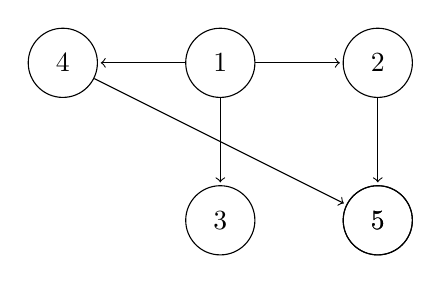
\begin{tikzpicture}[shorten >=1pt, node distance=2cm, on grid, auto]
	    \node[state] (q) {$1$};
 	    \node[state] (q_0) [left=of q] {$4$};
	    \node[state] (q_1) [right=of q] {$2$};
	    \node[state] (q_2) [below=of q] {$3$};
	    \node[state] (q_0_1) [below=of q_1] {$5$};
	    \node[state] (q_1_0) [below=of q_1] {$5$};

	    \path[->]
	    (q) edge node {} (q_0)
	    (q) edge node {} (q_1)
	    (q) edge node {} (q_2)
	    (q_0) edge node {} (q_0_1)
	    (q_1) edge node {} (q_1_0); 
	\end{tikzpicture}
	\item Queue Example with this graph:
	\begin{enumerate}
		\item First Level: [Lvl 0. | 1 - - - -]
		\item Next level: [Lvl 1. | - 2 3 4 -]
		\item Final level: [Lvl 2. | - - - - 5]
	\end{enumerate}
	\item And this is the Array Representation of this Queue/Graph leveling: [0, 1, 1, 1, 2]
\end{enumerate}

\vspace{1em}
\subsection*{Important Graph Info}
\begin{enumerate}
\item Further Graph Info:
	\begin{enumerate}
	\item Graph G = (V, E), $|V| = n$, $|E| = m$
		\begin{table}[h]
		\begin{tabular}{r|cc}
		Problem & \multicolumn{2}{l}{Adj. Matrix vs Adj. List}\\
		\hline
		Space & $O(n^2)$ & $O(n+m)$ \\
		$(U, V) \in E$ & $O(1)$ & $O(degree(u))$ \\
		Iterate Over (u, *) & $O(n)$ & $O(degree(u))$ \\
		BFS & $O(n^2)$ & $O(\sum_u degree(u))$ 
		\end{tabular}
		\end{table}
	\item Terminology:
		\begin{enumerate}
		\item \textbf{Sparse} represents a graph with a lack of nodes and connections between them. Sparse graphs are usually best examined in $O(n+m)$ time. 
		\item \textbf{Dense} represents a graph with a large amount of nodes and connections between them. Dense graphs are usually best examined in $O(n^2)$.
		\end{enumerate}
	\item The smallest possible $m$ (amount of edges) for a graph is 0. (A single node graph).
	\item The largest possible $m$ is $n*(n-1)/2$, where each node can have 2 edges at the sense of $n \choose 2$
	\item A $(U,V)$ is a graph node connection. 
	\item (u, *) represents a "connection between all nodes for u"
	\item Simplified explanation of Breadth First Search: Iterate over (u, *) for all Nodes v.
		\begin{enumerate}
		\item Best to think of it as a summation of all the degrees of u in the size of $m$ \underline{twice}, meaning you have to go through all $n$ nodes (the vertices), then through $m$ edges afterwards. 
		\end{enumerate}
	\item $O(\sum_u degree(u)) = O(n+m)$ essentially.
	\end{enumerate}
\end{enumerate}

\vspace{1em}
\begin{enumerate}
\item Simplified Lecture Notes:
	\begin{enumerate}
	\item \textbf{Connected components}: refers to all nodes that are reachable from a given node / vertex.
	\item A \textbf{\underline{Bipartite Graph}} is an undirected graph such that all edges can connect to all nodes that are of disjoint sets. 
		\begin{enumerate}
		\item For example:
		\item Consider a four node graph, where two nodes are blue and two nodes are red. 
		\item If there are existing undirected edges that connect to all nodes and...
		\item if each "end" of an edge is a different color, then the graph is Bipartite
		\end{enumerate}
		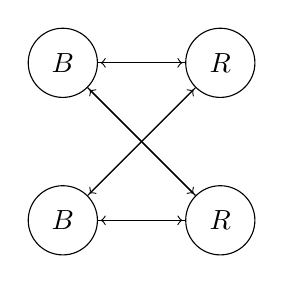
\begin{tikzpicture}[shorten >=1pt, node distance=2cm, on grid, auto]
	    	\node[state] (q) {$R$};
 	    	\node[state] (q_0) [left=of q] {$B$};
	    	\node[state] (q_1) [below=of q_0] {$B$};
	    	\node[state] (q_2) [below=of q] {$R$};

	    	\path[->]
	    	(q) edge node {} (q_0)
	    	(q) edge node {} (q_1)
	    	(q_0) edge node {} (q)
	    	(q_0) edge node {} (q_2)
		(q_2) edge node {} (q_0)
		(q_1) edge node {} (q_2)
		(q_1) edge node {} (q)
		(q_2) edge node {} (q_1);
		\end{tikzpicture}
		\begin{enumerate}
		\item Problems are generally easier to solve when the graph is bipartite.
		\item Must re-iterate, a \textbf{bipartite graph} is a graph where nodes can be separated into disjoint sets, and all edges distinctly point to disjoint nodes.
		\item Proof of that no bipartite graph can contain an odd length cycle:
			\begin{enumerate}
			\item The edges must alternate between nodes of different colors, but with an odd length of edges that is impossible, there will always result a link between nodes of like color. 
			\end{enumerate}
		\end{enumerate}
		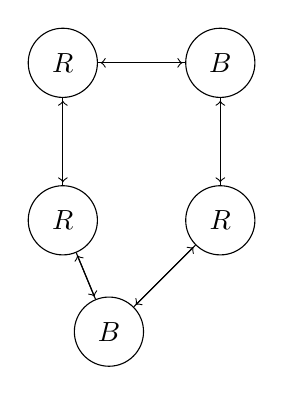
\begin{tikzpicture}[shorten >=1pt, node distance=2cm, on grid, auto]
	    	\node[state] (q) {$B$};
 	    	\node[state] (q_0) [left=of q] {$R$};
	    	\node[state] (q_1) [below=of q_0] {$R$};
	    	\node[state] (q_2) [below=of q] {$R$};
		\node[state] (q_3) [below left=of q_2] {$B$};

	    	\path[->]
	    	(q) edge node {} (q_0)
	    	(q) edge node {} (q_2)
	    	(q_0) edge node {} (q)
		(q_0) edge node {} (q_1)
		(q_1) edge node {} (q_0)
		(q_1) edge node {} (q_3)
		(q_2) edge node {} (q)
		(q_2) edge node {} (q_3)
		(q_3) edge node {} (q_2)
		(q_3) edge node {} (q_1);
		\end{tikzpicture}
	\item Additionally, if a Graph is Bipartite, the following principles hold:
		\begin{enumerate}
		\item No edge of Graph G can join 2 nodes of different layers or \textbf{levels} --> Bipartite
		\item If an edge of Graph G joins two nodes of the same layer, then that would result in an Odd Length Cycle
		\end{enumerate}
	\item A BFS will determine the bipartiteness of a graph, because there factually cannot be an edge in the same layer between nodes.
	\item There are K edges out from a vertex node that cycle back (which is always even). 
	\item K+1 edges, (such as if they are between nodes in the same layer) result in an odd length.
	\item Point is: [Edge in the same layer] -> [Odd length cycle] -> [Not a Bipartite graph]
	\item A BFS must have single connections between nodes (i.e a graph can't be squared or have edges spanning more than 1 node)
	\end{enumerate}
\vspace{1em}
\item Directed Graphs:
	\begin{enumerate}
	\item Connectivity differs in the sence of \textbf{Strong Connectivity}
	\item \textbf{Strong connectivity}: Mutual reachability between nodes --> Every node can reach each other.
	\item A graph can be determined strongly in $O(m+n)$ time. 
		\begin{enumerate}
		\item Pick a node
		\item Do BFS in Graph G on Node S
		\item Do Bfs on the Reverse of Graph G on Node S
		\item \textbf{Iff all nodes reached in both BFS, then the graph is strongly connected}
		\end{enumerate}
	\end{enumerate}
\end{enumerate}	

\subsection*{February 2nd - Continuation of Graphs} 
\begin{enumerate}
\item More Directed Graphs:
	\begin{enumerate}
	\item Example of a Directed Graph that is \textbf{not} strongly connected: \\
	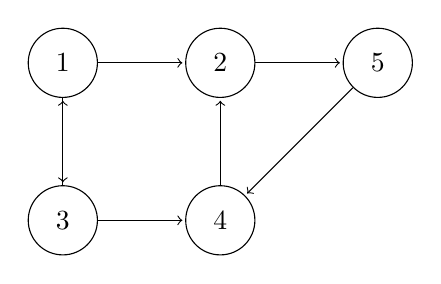
\begin{tikzpicture}[shorten >=1pt, node distance=2cm, on grid, auto]
	    	\node[state] (q) {$2$};
 	    	\node[state] (q_0) [left=of q] {$1$};
	    	\node[state] (q_1) [below=of q_0] {$3$};
	    	\node[state] (q_2) [below=of q] {$4$};
		\node[state] (q_3) [right=of q] {$5$};

	    	\path[->]
	    	(q) edge node {} (q_3)
	    	(q_0) edge node {} (q)
		(q_0) edge node {} (q_1)
		(q_1) edge node {} (q_0)
		(q_1) edge node {} (q_2)
		(q_2) edge node {} (q)
		(q_3) edge node {} (q_2);
		\end{tikzpicture}
	\item All nodes in the graph \textbf{cannot} be examined from any arbitrary starting node 
	\item An \textbf{adjacency list} interpretation of this graph: 
		\begin{tabular}{|r|c|c|}
		\hline
		Node & \multicolumn{2}{l|}{Edges}\\
		\hline
		1 & -> 2 & -> 3 \\
		\hline
		2 & -> 5 & \\
		\hline
		3 & -> 4 & -> 1 \\
		\hline
		4 & -> 2 & \\ 
		\hline
		5 & -> 4 & \\
		\hline
		\end{tabular}
	\item And a \textbf{reverse adjacency list} is the following:
		\begin{tabular}{|r|c|c|}
		\hline
		Node & \multicolumn{2}{l|}{Edges}\\
		\hline
		1 & -> 3 &  \\
		\hline
		2 & -> 4 & -> 1\\
		\hline
		3 & -> 1 & \\
		\hline
		4 & -> 5 & -> 3\\ 
		\hline
		5 & -> 2 & \\
		\hline
		\end{tabular}
	\item Reverse Adjacency List Process: 
		\begin{enumerate}
		\item Firstly, when a node's linked list is empty, simply insert the inverse of each node
		\item When a node's list is \textbf{not} empty, insert the "next" node \textbf{first}, in front of the other existing nodes in the list
		\item Carefully study how nodes 2 and 4 are in two node's lists in the original Adjacency list. The inverse means those two nodes are now in their lists.
		\end{enumerate}
	\end{enumerate}
\item \textbf{Directed Acyclic Graph}
	\begin{enumerate}
	\item A directed graph with no directed cycles is called an \textbf{directed acyclic graph}. This follows the constraint that $Edge(V_{i}, V_{j})$ must have Node $V_{i}$ precede Node $V_{j}$.  
	\end{enumerate}
\item \textbf{Topological Order} 
	\begin{enumerate}
	\item \textbf{Topological ordering} of a directed Graph G = (V, E) is an ordering of nodes $(1...n)$ where $i < j$ for every Node $V_{i}$ followed by Node $V_{j}$.
	\item Basically, every node must be followed by a node "greater than it" in the ordering. Then just connect the edges according to how they were connected in the original graph.
	\item Example with Nodes going Left -> Right: \\\\
	\begin {tikzpicture}[-latex, auto, node distance = 1 cm and 2 cm, on grid, semithick, state/.style ={ circle, top color =white, bottom color = processblue!20, draw, processblue, text = blue, minimum width =1 cm}]
	\node[state] (A) {$1$};
	\node[state] (B) [right=of A] {$2$};
	\node[state] (C) [right =of B] {$3$};
	\node[state] (D) [right =of C] {$4$};
	\node[state] (E) [right =of D] {$5$};
	
	\path (A) edge [bend right =35] node[right] {} (C);
	\path (A) edge [bend right = 45] node[below =0.15 cm] {} (D);
	\path (B) edge [right] node[below = 0.00 cm] {} (C);
	\path (B) edge [bend left =25] node[below =0.15 cm] {} (E);
	\path (C) edge [right] node[below =0.00 cm] {} (D);
	\path (D) edge [right] node[below =0.00 cm] {} (E);
	\end{tikzpicture}
	\item Usually, one topological ordering is sufficient, even if there may be more than one way to do so.
	\item \textbf{Important:} If there exists a cycle in the graph, a Topological Ordering is \textbf{not possible}.
	\item Therefore, there are three principles that are intertwined:
		\begin{enumerate}
		\item If there is a Topological Ordering, then the Graph is a DAG.
			\begin{enumerate}
			\item Proof by Contradiction: There must be a cycle if it isn't a DAG. But you can't topologlically order a graph if there is a cycle. Boom roasted. 
			\end{enumerate}
		\item If the Graph G is a DAG, then there is a node with no incoming edges (A "first/root" node) 
			\begin{enumerate}
			\item Proof by Contradiction: All edges must have an incoming edge. But if that were true, you could trace back indefinitely in a loop. Aka, a cycle. And DAG's can't have those. 
			\end{enumerate}
		\item Lastly, if G is a DAG, on $i$ vertices, it has a topological ordering. The proof of this I will cover in a following section after an example of a Topological DAG.
		\item Firstly, another example of a DAG: \\\\
		\begin {tikzpicture}[-latex, auto, node distance = 1.5 cm and 2 cm, on grid, semithick, state/.style ={ circle, top color =white, bottom color = processblue!20, draw, processblue, text = blue, minimum width =1 cm}]
		\node[state] (A) {$1$};
		\node[state] (B) [above left=of A] {$5$};
		\node[state] (C) [below left =of B] {$7$};
		\node[state] (D) [above right =of A] {$4$};
		\node[state] (E) [above left =of D] {$3$};
		\node[state] (F) [above left =of B] {$2$};
		\node[state] (G) [below left =of F] {$6$};
	
		\path (A) edge [left] node[above =0.00 cm] {} (B);
		\path (A) edge [left] node[below =0.00 cm] {} (C);
		\path (A) edge [right] node[above = 0.00 cm] {} (D);
		\path (B) edge [left] node[below =0.00 cm] {} (G);
		\path (B) edge [left] node[below =0.00 cm] {} (C);
		\path (D) edge [left] node[below =0.00 cm] {} (B);
		\path (E) edge [right] node[below =0.00 cm] {} (D);
		\path (E) edge [right] node[below =0.00 cm] {} (B);
		\path (F) edge [right] node[below =0.00 cm] {} (E);
		\path (F) edge [right] node[below =0.00 cm] {} (B);
		\path (F) edge [right] node[below =0.00 cm] {} (G);
		\path (G) edge [right] node[below =0.00 cm] {} (C);
		\end{tikzpicture}
		\item And now a Topological Ordering of this DAG: \\\\
		\begin {tikzpicture}[-latex, auto, node distance = 1.5 cm and 2 cm, on grid, semithick, state/.style ={ circle, top color =white, bottom color = processblue!20, draw, processblue, text = blue, minimum width =1 cm}]
		\node[state] (A) {$1$};
		\node[state] (B) [right =of A] {$2$};
		\node[state] (C) [right=of B] {$3$};
		\node[state] (D) [right =of C] {$4$};
		\node[state] (E) [right =of D] {$5$};
		\node[state] (F) [right =of E] {$6$};
		\node[state] (G) [right =of F] {$7$};
	
		\path (A) edge [bend right = 25] node[below =0.40 cm] {} (D);
		\path (A) edge [bend right = 30] node[below =0.45 cm] {} (E);
		\path (A) edge [bend right = 35] node[below =0.50 cm] {} (G);
		\path (B) edge [right] node[below =0.00 cm] {} (C);
		\path (B) edge [bend left = 32] node[above =0.50 cm] {} (E);
		\path (B) edge [bend left = 35] node[below =0.50 cm] {} (F);
		\path (C) edge [bend left = 27] node[below =0.50 cm] {} (E);
		\path (C) edge [right] node[below =0.50 cm] {} (D);
		\path (D) edge [right] node[below =0.50 cm] {} (E);
		\path (E) edge [right] node[below =0.50 cm] {} (F);
		\path (E) edge [bend right = 25] node[below =0.50 cm] {} (G);
		\path (F) edge [right] node[below =0.50 cm] {} (G);
		\end{tikzpicture}
		\end{enumerate}
	\item And now I will prove that third Lemma by introduction of the 5 Step Proof process.
	\item Also, as quick aside: $\forall (x)$ means "For all existing $x$" and $\exists (x)$ means "There exists a particular case of $x$"
	\end{enumerate}
\item \textbf{\underline{5 Step Proof Process}}: 
	\begin{enumerate}
	\item $\forall (i)$ Prove each $i$ (Referenced as $P(i)$) by Induction
	\item Provide a Base Case (For example, a 1 node graph)
	\item Assume $P(i)$ is true $\forall (i \leq j)$. Prove $P(j+1)$ induction.
	\item Provide a proof implementation (i.e put your proof into words and mathematical principles).
	\item Apply Inductive Hypothesis in Proof (Noted as $G'$ in the following example). 
	\end{enumerate}
\item And now to exemplify this, here is the proof of the third principle of DAGs and Topological Ordering mentioned above:
	\begin{enumerate}
	\item We have a Graph G that has $j+1$ vertices and is a DAG.
	\item We know via the lemmas proven that: there must $\exists(v)$ where $v$ is a node that has no incoming edges for a topological ordering.
	\item Inductive Hypothesis: Create a Graph $G'$ such that it has $j$ nodes (one less than the current G) and is a DAG with a topological ordering.
	\item Now \textbf{prepend} another node, which would be $j+1$, to this graph. Well...
	\item Since we already have a node with no incoming edges, if we \textbf{prepend} the new node to the current graph, we will just put another node at the beginning of the topological order with no incoming edges.
	\item Therefore, this graph G with the newly prepended $j+1$ node will be a topologically ordered Graph.
	\item And if you keep doing this via the Inductive Hypothesis, then we have successfully shown that any additional node will just further satisfy the Graph G as a topological ordering.
	\item Hurray. 
	\end{enumerate}
\item As a practical note, it is \textbf{necessary} to formalize all of these items in both your homeworks and your tests. You will be marked down otherwise. 
\item Also, in the proof above, $G'$ was a DAG because we assumed G was a DAG and were only able to remove nodes with outbound edges. It is vital that assumptions like this are clarified in proofs.
\item Algorithmic time complexity of Topological Order: $O(m+n)$
\item Algorithm for Topological Order:
	\begin{enumerate}
	\item Need a count for the remaining edges
	\item Also intialize a set with node that do not have incoming edges
	\item Begin by scanning the graph once ($O(n+m)$)
	\item Then begin updating: Delete a Node v, decrement the count for all of Node v's edges, and add the endpoint nodes when the count hits 0 to the set
	\item All of this takes $O(1)$ time per edge.
	\end{enumerate}
\item And that about finishes this portion of Graph information
\end{enumerate}

\vspace{1em}
\subsection*{Greedy\textsuperscript{TM} Algorithms}
\begin{enumerate}
\item \textbf{Greedy\textsuperscript{TM} Algorithms} are understood as Algorithms that take the best first/immediate solution to a problem as they arise. There ain't much goin' ons up in the ol' noodle for these.
\item For example, the \textbf{Job Problem}: Need as many jobs to be filled as possible while taking as much time out a schedule as possible.
	\begin{enumerate}
	\item Jobs must be mutually compatible, there can be no overlap between jobs in a schedule.
	\end{enumerate}
\item The Greedy\textsuperscript{TM} Approach:
	\begin{enumerate}
	\item Take the jobs as they come naturally, so long as they are sequentially compatible to one another (i.e. pick one job, and then when it's finished, pick the next available job)
	\item There are four ways of thinking about this:
		\begin{enumerate}
		\item Earliest Start Time
		\item Earliest Finish Time
		\item Shortest Intervals
		\item Fewest conflicts
		\end{enumerate}
	\item When searching for a counterrexample, always take the shortest/smallest possible.
	\item Out of the 4 ways of analyzing this algorithm, only one works: Earliest Finish Time.
	\item So the Algorithm is as follows:
		\begin{enumerate}
		\item Sort the jobs in the schedule by finish time ($O(n * log(n))$)
		\item Then parse through each job in the schedule, finding the ones that are most compatible according to finish time. Example: A job has a start time of $s_{i}$ and a finish time of $s_{i}$. The next job has a start time of $s_{j}$ and a finish time of $f_{j}$. To find compatibility, just check if $s_{j}$ of Job 2 comes before $f_{i}$ of Job 1. 
		\item Overall time complexity: $O(n * log(n))$
		\end{enumerate}
	\end{enumerate}
\item The proof of this algorithm is extremely important (and very relevant to a lot we'll cover with Greedy\textsuperscript{TM} Algorithms). It is -- as Professor Byers put it -- \textbf{Subtle, Short, \& Nuanced}. How poetic. 
	\begin{enumerate}
	\item Proof By Contradiction: Suppose that the current Greedy\textsuperscript{TM} Algorithm we've devised is \textbf{not the optimal solution}
		\begin{enumerate}
		\item Let $i$, ranging from $(1...k)$, be a set of jobs devised by our Greedy\textsuperscript{TM} approach.
		\item Les $j$, ranging from $(1...m)$, be a set of jobs from the supposed \textit{true optimal solution}
		\item Let the association between $i$ and $j$ be as such: $i_{1} = j_{1}$,  $i_{2} = j_{2}$, {...}  $i_{r} = j_{r}$, where $r$ represents the furthest possible point $i$ and $j$ are identical sets.
			\begin{enumerate}
			\item Greedy\textsuperscript{TM} : 
			\begin {tikzpicture}[-latex, auto, node distance = 0 cm and 2 cm, on grid, semithick, state/.style ={ rectangle, top color =white, bottom color = processblue!20, draw, processblue, text = blue, minimum width =1 cm}]
			\node[state] (A) {$i_{1}$};
			\node[state] (B) [right =of A] {$i_{2}$};
			\node[state] (C) [right=of B] {$i_{3}$};
			\node[state] (D) [right =of C] {$i_{r}$};
			\node[rectangle, top color =white, bottom color = processblue!20, draw, processblue, text = blue, minimum width =2 cm] (E) [right =of D] {$i_{r+1}$};

			\path (A) edge [left] node[below =0.00 cm] {} (B);
			\path (B) edge [left] node[below =0.00 cm] {} (C);
			\path (C) edge [left] node[below =0.00 cm] {} (D);
			\path (D) edge [left] node[below =0.00 cm] {} (E);
			\end{tikzpicture}
			\item Optimal\textsuperscript{TM}: 
			\begin {tikzpicture}[-latex, auto, node distance = 0 cm and 2 cm, on grid, semithick, state/.style ={ rectangle, top color =white, bottom color = processblue!20, draw, processblue, text = blue, minimum width =1 cm}]
			\node[state] (A) {$j_{1}$};
			\node[state] (B) [right =of A] {$j_{2}$};
			\node[state] (C) [right=of B] {$j_{3}$};
			\node[state] (D) [right =of C] {$j_{r}$};
			\node[state] (E) [right =of D] {$j_{r+1}$};

			\path (A) edge [left] node[below =0.00 cm] {} (B);
			\path (B) edge [left] node[below =0.00 cm] {} (C);
			\path (C) edge [left] node[below =0.00 cm] {} (D);
			\path (D) edge [left] node[below =0.00 cm] {} (E);
			\end{tikzpicture}
			\end{enumerate}
		\item To put it bluntly, because $j_{r+1}$ has a differing start/finish time, that is suppose to be where the optimality comes in. 
		\item Yet, substituting in $i_{r+1}$, which generally has an earlier start time and a later finish time, would be just as optimal. 
		\item So therefore, there is essentially no better/more optimal way of beating out the Greedy\textsuperscript{TM} solution.
		\end{enumerate}
	\item This proof can be generalized to the following saying that applies to most Greedy\textsuperscript{TM} Algorithms: \\\\ \textbf{\textit{\Large{"Greedy Stays Ahead"}}} \vspace{.5em}
	\item Also, this Job Problem can be found under the umbrella of a series of Greedy\textsuperscript{TM} Problems called \textbf{Interval Scheduling Problems}.
	\end{enumerate}
\item On that note, going further into Greedy\textsuperscript{TM} problems, we approach the \textbf{Interval Partitioning} problems:
	\begin{enumerate}
	\item Given a set of classes and a set of classrooms, find a schedule where no two classes occur in the same room simultaneously, and use the fewest amount of rooms possible.
	\item \textbf{Important Terminology Alert}: \textbf{\underline{Depth}} in this case means the maximum number of sets of open intervals in the schedule at any given time. (i.e. a point in the schedule where there's nothing occurring)
	\item If the \textbf{number of classrooms used} matches the \textbf{depth}, then you have found the optimal solution. 
	\item The Greedy\textsuperscript{TM} Approach:
		\begin{enumerate}
		\item Consider lectures in order of increasing starting times. 
		\item Assign each class to a compatible classroom. If a class ends before the next starting class time, re-use this classroom. 
		\item If there is a conflict of existing classrooms (i.e the next class starts while the other class is still in session in that classroom), then assign a new classroom to this new class. 
		\item Time complexity for this: $O(n * log(n))$
		\item Implementation:
\begin{python}
Sort by starting time in a priority queue (earliest to latest)
for lecture in range(1, n):
  if(room & lecture are compatible):
    assign lecture to classroom
  else
    get a new room
    put lecture in this new room
    old_room -> new_room
 \end{python}
		\item Sort time: $O(n * log(n))$
		\item For loop: $O(n)$
		\item Class assignment where $f_{i} \leq s_{j}$ : $O(c)$ <-- Some constant factor
		\item \underline{Observe} that this algorithm never overlaps classes.
		\item Proof:
			\begin{enumerate}
			\item Let $d$ equal total number of classrooms.
			\item Let the first class, represented as $j-1$ be starting in room 1 which is $d-1$.
			\item Then let the final class be starting at $j$ in the final room $d$.
			\item Then suppose that $j + \varepsilon$ time passes, where $\varepsilon$ represents a small, near negligible, value but still shows that $j + \varepsilon > j$. 
			\item Then that means all possible classrooms are being used simultaneously by all possible classes. 
			\item So the \textbf{key note} here is that all schedules will use $\geq d$ classrooms.
			\end{enumerate}
		\end{enumerate} 
	\end{enumerate} 
\item The next Greedy\textsuperscript{TM} problem is the \textbf{Minimizing Latness} problem:
	\begin{enumerate}
	\item Goal: Schedule all jobs to minimize maximum lateness, where $L$ = $max l_{j}$
	\item Job $j$ requires $t_{j}$ time and is due at $d_{j}$ hour. It also starts at $s_{j}$ and finishes at: $f_{j} = s_{j} + t_{j}$
	\item \textbf{Lateness} is denoted as: $l_{j}$ = $max\{0, f_{j} - d_{j}\}$
	\item Possible ways of solving:
		\begin{enumerate}
		\item Earliest deadline first
		\item Smallest time first, unless a deadline is approaching, then that immediate job takes priority.
		\item Shortest processing time
		\item Smallest Slack (Slack = Least amount of worry about deadline approaching + time it takes to finish)
		\end{enumerate}
	\item Conclusion: Earliest Deadline First is the best approach (go figure)
	\item Implementation:
\begin{python}
Sort by deadline time intervals
for job in range(1, n)
  Assign job to a time
  Compute start time and finish time
  Then go from the next time interval
Output the listing
\end{python}
	\item Overall Time Complexity: $O(n)$ 
	\item No idle constant time or anything, just a straightforward way of doing things.
	\item New proof technique for this: \textbf{\textit{Exchange Argument}}
		\begin{enumerate}
		\item Invert a Greedy\textsuperscript{TM} devised schule S such that a pair of jobs swap placement and time. (Such that $i < j$ yet $j$ is scheduled before $i$)
		\item There may be other inversions also, but this case should show for all.
		\item Claim: There is no lateness change
			\begin{enumerate}
			\item First, remember that \textit{Lateness = Finish time - Deadline time}
			\item $l$ represents the lateness before the swap, and $l'$ represents afterwards
			\item We know that $l_{i} \leq l'_{i}$ 
			\item Then $l'_{j} = f'_{j} - d_{j}$. However, $f'_{j}$ is just the swapped finish time of $i$, so it's really --> $l'_{j} = f_{i} - d_{j}$
			\item HOWEVER, we know that $j$ must be scheduled at a later deadline, so it's difference between finish and deadline time is less than that of i
			\item So, $l'_{j} \leq f_{i} - d_{j}$
			\item And $f_{i} - d_{j}$ is literally just $l_{i}$, so $l'_{j} \leq l_{i}$, proving that there was no loss in lateness from the inversion of schedules
			\end{enumerate}
		\end{enumerate}
	\item In short, the latness of this new swap of Job $j$ will note be greater than the latness of the original Job $i$ in its place.
	\item This lateness proof lends to the overall proof of the Algorithm:
		\begin{enumerate}
		\item Assume the Greedy\textsuperscript{TM} algorithm is $S$ and the Optimal solution is $S*$ with the fewest inversions possible.
		\item But we just proved inversions make no difference for the original algorith. So the effect of inversions results to 0. 
		\item However, if this is the case, then that contradicts that this $S*$ has the fewest inversions. Which leads to the fact the optimal solution is a schedule without inversions.
		\item Which is just $S$ 
		\end{enumerate}
	\end{enumerate}
\item Quick Recap on Greedy\textsuperscript{TM} Algorithm Proof techniques:
	\begin{enumerate}
	\item "Greedy Stays Ahead"
	\item Structural flaws -> Your algorithm can be shown to be optimal anyways, like the example above
	\item Exchange Argument
	\end{enumerate}
\item Finally, we arrive at the \textbf{Shortest Path Problem}:
	\begin{enumerate}
	\item Goal: Find the shortest route from Source $S$ to Destination $T$
	\item Quick Response: Assign values to all pathways, and find the smallest (read: best) summable path.
	\item \textbf{\large{Dijkstra's Algorithm}}
		\begin{enumerate}
		\item Maintain a set of nodes with the shortest path (Hint: Use a priorty queue)
		\item Begin a pre-processing analyzation of the graph with each outgoing edge from a node being assigned a value. These "values" are much like something as how long it takes to drive down a road.
		\item Assume the distance to each node is infinitely long at first, except at the source node.
		\item Then, as each node is explored, analyze outgoing edge values and determine which edge value is the smallest. The "travel time" from each node is thus the sum of edges from the starting node to the current node traveled.
		\item Each explored node should be inserted into a set $S$ of explored nodes.
		\item Smallest Distance: $\pi (v)$ = $SD(u)$ + $l_{e}$
			\begin{enumerate}
			\item $SD(u)$ = Smallest Distance from some node $u$
			\item $l_{e}$ = Total sum of edge weights thus far accumulated via the shortest path
			\item $\pi (v)$ = The next possible shortest distance path in the graph where $\pi (v) <$ all other edge weights of $v$
			\end{enumerate}
		\item After this calculation has been made, make sure the current node is updated to the new $\pi (v)$ node. 
		\end{enumerate}
	\end{enumerate}
\end{enumerate}

\vspace{1em}
\subsection*{Continuation of Greedy\textsuperscript{TM} Algorithms}
\begin{enumerate}
\item \textbf{Proof of Dijkstra's Algorithm:}
	\begin{enumerate}
	\item Claim: When a Node $u$ is added to the set of explored nodes, $S$, then it is true that the distance of Node $u = \pi (u)$, which is the shortest path.
		\begin{enumerate}
		\item Base Case: $|S|$ = 1 (meaning there's only 1 node in the graph). If $S = \{s\}$, then distance of the total edges in $S$ is: $d(s) = 0$.   
		\item Inductive Hypothesis: Therefore, assume that is true that $|S| = K \geq 1$, where $K$ is the arbitrary value denoting new nodes added to the set from its current state. Then if we insert a new Node $v$ into set $S$, it should follow that: $\pi (v) = l_{e} + d(u)$; $\pi (v) == d(v)$.
		\item So assume the contradiction: 
			\begin{enumerate}
			\item Suppose that there is a $P'$ such that $P' \neq P + U_{e}$, where $P$ would be the existing best short path and $U_{e}$ is the weight of Node $u$'s edges.
			\item Then you would have to suppose there exists some link from a node $x$ to a node $y$ such that it follows from pathway $P'$ to the node $v$.
			\item Graphically, it would look like this: \\
			\begin {tikzpicture}[-latex, auto, node distance = 2 cm and 2 cm, on grid, semithick, state/.style ={ circle, top color =white, bottom color = processblue!20, draw, processblue, text = blue, minimum width =1 cm}]
			\node[state] (A) {$s$};
			\node[state] (B) [above right =of A] {$x$};
			\node[state] (C) [below right=of A] {$u$};
			\node[circle, top color =white, bottom color = white, draw, processblue, text = blue, minimum width =1 cm] (D) [right =2cm and 4cm of C] {$v$};
			\node[circle, top color =white, bottom color = white, draw, processblue, text = blue, minimum width =1 cm] (E) [right =2cm and 4cm of B] {$y$};

			\path (A) edge [left] node[below =0.00 cm] {$P'$} (B);
			\path (A) edge [right] node[below =0.20 cm] {$P$} (C);
			\path (B) edge [dotted] node[below =0.00 cm] {} (E);
			\path (C) edge [left] node[below =0.00 cm] {$l_{e}$} (D);
			\path (E) edge [dotted] node[below =0.00 cm] {} (D);
			\end{tikzpicture}
			\item The nodes shaded in blue are explored nodes that belong to set $S$. The white nodes are the unexplored nodes that can be reached in the graph. 
			\item What this graph basically indicates is an "alternate path" to this node $v$ that is proposed to be better than Node $u$ through pathway $P$. 
			\item Mathematically, the contradiction can be viewed this way: \\\\ $l(P) \geq l'(P') + l(x,y) \geq d(x) + l(x,y) \geq \pi(y) \geq \pi(v)$ \\
			\item The first $\geq$ refers to the non-negative weights of the Pathways of $P$ and $P'$. The second one refers to the Inductive Hypothesis we proposed, where all pathways with +1 greater edges are greater than the current node's pathways. The third refers to the definitive/calculable shortest distance to Node $y$. And the final $\geq$ refers to the pathway that Dijkstra's algorithm calculated was the shortest pathway to Node $v$. \\
			\end{enumerate}
		\item Basically, what all this mean is that if Dijkstra's algorithm found a pathway to $v$ that was appreciatively smaller than all other pathways, then this contradicatory pathway $P'$ cannot possibly serve as a better alternative route. This is predicated on the fact that the next shortest path to $v$ from some pathway with node $x$ must go through some node $y$, when we could already reach $v$ directly from $u$.
		\end{enumerate}
	\end{enumerate}
\item Implementation:
	\begin{enumerate}
	\item For each unexplored node...
		\begin{enumerate}
		\item Continually update the $\pi(v)$ minimum function as you explore.
		\item Pretty easy, no?
		\end{enumerate}
	\item Essentially: \\ $\pi(new)$ = \textbf{IF} edge $(v, u)$ is in Edge Set $E$ \textbf{THEN} $d(u) + l(u,v)$ \textbf{ELSE} $\pi_{old}(v)$ 
	\end{enumerate}
\item Efficient Implementation:
	\begin{enumerate}
	\item Maintain a Priority Queue of unexplored nodes that are prioritized based on their shortest distance: $\pi(v)$.
	\item Designate operations per search of a node with PQ.minimum() and PQ.updateKey($\pi_{old}(v), \pi_{new}(v)$).
	\item Whenever we update nodes, we have $m$ edge examinations.
	\item So with a binary heap: $m * log(n)$ operations per.
		\begin{enumerate}
		\item Initialize Set: $O(n)$  -- Preprocess
		\item Initialize PQ: $O(n*log(n))$ -- Preprocess
		\item for i = 1...n: 
			\begin{enumerate}
			\item PQ.min: $O(n*log(n))$ -- Additive
			\item PQ.updK: $O(m*log(n))$ -- Additive
			\end{enumerate}
		\end{enumerate}
	\item Thus, the overall time complexity is $O(m * log(n))$
	\end{enumerate}
\item Quick Review on Trees:
	\begin{enumerate}
	\item A graph G= (V,E) is a tree iff;
		\begin{enumerate}
		\item It is connected
		\item Does not contain any cycles.
		\end{enumerate}	
	\item Things we know about trees:
		\begin{enumerate}
		\item The number of edges is always 1 less than the number of nodes ($m = n-1$)
		\item A tree has at least 2 leaves.
		\end{enumerate}
	\item A graph is a DAG if it shares the same two properties: It is connected and does not contain any cycles. Therefore, there is an existing relationship between a DAG and a Tree.
	\end{enumerate}
\item \textbf{\large{Minimum Spanning Trees}}
	\begin{enumerate}
	\item Definition: Given a Graph $G$, an MST is just a subset of nodes such that it is the smallest tree inside of $G$.
	\item Incredibly important Data Structure with a multitude of applications.
	\item Formal understanding: Given a graph G = (V,E) with valued weights $c_{e}$, an MST is a subset where $T \subseteq E$ such that $T$ is a tree whose sum is minimized.
	\item Algorithm Strategizing: 	
		\begin{enumerate}
		\item Reverse-Delete Theorem: Start with all edges and delete from the heaviest weight trending down. 
		\item Prim's Algorithm: Start with a root node, then greedily choose the best path based on total weight, much like Dijkstra's.
		\item Kruskal's Theorem: Best to examine edges by increasing weight per node, $l_{e_{1}} \leq l_{e_{2}} \leq ... \leq l_{e_{n}}$
		\end{enumerate}
	\item All three of these Algorithms work. However, Reverse-Delete is somewhat ineficient, so we'll only truly worry about Kruskal and Prim's. 
	\item Very Important Notes:
		\begin{enumerate}
		\item Simplified Assumption: Edge weights are all distinct ($c_{e}$ are all different).
		\item \textbf{Cut Property}: A set $S$ is a subset of nodes, edge $e$ is the minimum cost edge with exactly 1 endpoint $S$. Then the MST must contain this edge $e$.
		\item \textbf{Cycle Property}: A cycle $C$ is any cycle in the Graph, let edge $f$ be the maximum edge cost in the Cycle $C$. Then the MST must \textbf{not} contain this edge $f$.
		\item Following graph: (Blue = Within set $S$, White = Unexplored nodes). \\
		\begin {tikzpicture}[-latex, auto, node distance = 2 cm and 2cm, on grid, semithick, state/.style ={ circle, top color =white, bottom color = processblue!20, draw, processblue, text = blue, minimum width =1 cm}]
			\node[state] (A) {};
			\node[state] (B) [below right =of A] {};
			\node[state] (C) [below =4cm and 4cm of A] {};
			\node[circle, top color =white, bottom color = white, draw, processblue, text = blue, minimum width =1 cm] (D) [right =2cm and 6cm of A] {};
			\node[circle, top color =white, bottom color = white, draw, processblue, text = blue, minimum width =1 cm] (E) [right =1cm and 2cm of B] {};
			\node[circle, top color =white, bottom color = white, draw, processblue, text = blue, minimum width =1 cm] (F) [right =2cm and 5cm of C] {};
	
			\path (A) edge [left] node[below right =0.00 cm] {} (B);
			\path (A) edge [right] node[below =0.00 cm] {} (C);
			\path (A) edge [dotted] node[below =0.00 cm] {$f$} (D);
			\path (B) edge [dotted] node[below =0.00 cm] {$e$} (E);
			\path (B) edge [left] node[above =0.00 cm] {} (A);
			\path (C) edge [dotted] node[below =0.00 cm] {} (F);
			\path (C) edge [right] node[above =0.00 cm] {} (A);
			\path (D) edge [left] node[below =0.00 cm] {} (F);
			\path (F) edge [left] node[below =0.00 cm] {} (D);
		\end{tikzpicture}
		\item Cycle-Cut Intersection -> There is a cross between both the Cycle Property and the Cut Property within a graph. The edges of the graph will always be even in this case. 
		\item A cycle cannot cross a cutset only once. It is impossible, as in order for a cycle to be complete, the edges have to eventually circle back to a certain node. So, there's a guarantee that parsing through a cycle will cross the cutset \textbf{at least twice}.
		\item \textbf{Proof of Cut and Cycle Properties}: (Use an Exchange Argument)
			\begin{enumerate}
			\item Suppose $e$ is not in the MST Tree $T$.
			\item Then let this correpsonding $e$ create a cycle in T.
			\item Therefore, $e$ is in the cycle $C$ and in the Cutset $D$ corresponding to the explored Set $S$. Let $c_{e}$, the edge weight for edge $e$, be less than $c_{f}$, the edge weight for another edge $f$ that apparently holds both the properties that $e$ holds. 
			\item So both $e$ and $f$ are in the Cutset $D$ and the Cycle $C$. And this is critical: these two existing in the Tree $T$ simultaneously are what generate the complete cycle. 
			\item $T'$ = $T \cup \{e\} - \{f\}$ is also an Minimum Spanning Tree. This Tree $T'$ holds all over the properties of that original Tree $T$, without edge $f$. 
			\item But since $c_{e} > c_{f}$, then $T' < T$ in cost. 
			\item Yet this does not make sense, since $T$ is supposed to be the Minimum Spanning Tree that was calculated to have the least weight. 
			\item So, $T'$ is actually the real $T$ that includes $e$ but not $f$ and removes the cycle and weighs the least possible. 
			\item And just to recall, both $T$ and $T'$ are trees that are \textbf{completely connected and with $m = n-1$ edges}. \\
			\begin {tikzpicture}[-latex, auto, node distance = 2 cm and 2cm, on grid, semithick, state/.style ={ circle, top color =white, bottom color = processblue!20, draw, processblue, text = blue, minimum width =1 cm}]
				\node[state] (A) {};
				\node[state] (B) [above right =of A] {};
				\node[state] (G) [right =of A] {};
				\node[state] (C) [below  =2cm and 2cm of A] {};
				\node[circle, top color =white, bottom color = white, draw, processblue, text = blue, minimum width =1 cm] (D) [right =2cm and 6cm of B] {};
				\node[circle, top color =white, bottom color = white, draw, processblue, text = blue, minimum width =1 cm] (E) [below right =2cm and 2cm of B] {};
				\node[circle, top color =white, bottom color = white, draw, processblue, text = blue, minimum width =1 cm] (F) [right =2cm and 4cm of C] {};
	
				\path (A) edge [left] node[below right =0.00 cm] {} (B);
				\path (A) edge [right] node[below =0.00 cm] {} (C);
				\path (A) edge [right] node[below =0.00 cm] {} (G);
				\path (G) edge [right] node[below =0.00 cm] {} (A);
				\path (B) edge [dotted] node[below =0.00 cm] {$f$} (D);
				\path (B) edge [left] node[above =0.00 cm] {} (A);
				\path (C) edge [dotted] node[below =0.00 cm] {$e$} (F);
				\path (C) edge [right] node[above =0.00 cm] {} (A);
				\path (D) edge [left] node[below =0.00 cm] {} (F);
				\path (F) edge [left] node[below =0.00 cm] {} (D);
				\path (E) edge [right] node[above =0.00 cm] {} (D);
				\path (D) edge [right] node[below =0.00 cm] {} (E);
			\end{tikzpicture}
			\end{enumerate}
		\item This proof works both for the Cycle property and the Cut property. The difference is between "supposing $e$ is not in $T$" versus "supposing $f$ belongs to $T'$" and then just coming to the conclusion that (because both $e$ and $f$ must be in the non-optimal tree and that $c_{e} < c_{f}$) removing $f$ and/or injecting $e$ into the Tree $T/T'$ is what would be the best possible MST. 
		\item In Summary:
			\begin{enumerate}
			\item $f$ and $e$ form a cycle within MST Tree $T$. Both of these edges are inclusive to the Cycle $C$ and the Cutset $D$.
			\item $c_{e} < c_{f}$
			\item Remove $c_{f}$ to remove the cycle from $T$
			\item Therefore, $T$ must have $e$.
			\end{enumerate}
		\end{enumerate}
	\end{enumerate}
\end{enumerate}

\vspace{1em}
\subsection*{February 16th - Continuation of Greedy\textsuperscript{TM} Algorithms}
\begin{enumerate}
\item \textbf{More on Minimum Spanning Trees}:
	\begin{enumerate}
	\item \textbf{Dijkstra's}: Finding the shortest path in a tree from a source node $s$ to a destination node $t$.
	\item \textbf{Minimum Spanning Tree}: Finding a Tree within a graph that minimize the amount of edges yet still maintains connection across all nodes. 
	\item In a sense, Dijkstra's is more about starting at a certain node, and then slowly branching out in the shortest path possible until a node is found. Not all edges need to be searched, nor does the path have to connect all nodes. And these points differ for MSTs.
	\item Note the difference, it could save your life! (maybe idk)
	\item Also, here lies a distinction between the two halves of the Greedy\textsuperscript{TM} Algorithms Chapter:
		\begin{enumerate}
		\item The first half is mostly about introducing elementary problems to provide concrete examples of Greedy\textsuperscript{TM} Algorithm proofs.
		\item The second half is mostly about introducing critically important and extremely common Greedy Algorithms (Dijkstra's, MSTs, Huffman Codes (To be seen) ), their implementations, and specific properties of their proofs that are generally applicable eslewhere. 	
		\end{enumerate}
	\item More In-Depth look at the MST Algorithms:
	\item Reverse-Delete:
		\begin{enumerate}
		\item Step 1: Repeatedly find a cycle on Graph $G$ ($O(m+n)$)
		\item Step 2: Delete the heaviest edge ($O(n)$)
		\item Step 3: Repeat this loop ($O(m-n-1)$ --> $O(m)$)
		\item Overall Time Complexity: $O(m^2)$ 
		\item Small Aside: $O(n) \leq O(m) \leq O(n^2)$ --> So take $O(m)$ as the upper bound.
		\item This algorithm is \textbf{not efficient}, and therefore not an algorithm you should focus on using in this class.   
		\end{enumerate}
	\item Prim's Algorithm:
		\begin{enumerate}
		\item Step 1: Initialize a set $S$. Begin at any arbitrary node.
		\item Step 2: Apply the cut property when searching for the shortest edge.
		\item Step 3: Add the minimum cost edge that was found from this to a Cutset  $Y$ corresponding to set $S$ into a Tree $T$ and add one new explored node $u$ to the set $S$.
		\item This is an efficient Algorithm that makes use of the Cut Property. 
		\item $n-1$ iterations, for $m$ edges.
		\item Implementation:
			\begin{enumerate}
			\item Startup a Priority Queue
			\item Maintain a set of explored nodes.
			\item Maintain cheapest edge costs to a node in a set.
			\item This is $O(n^2)$ with an array, $O(m*log(n))$ with a binary heap. 
			\item Pseudocode:
\begin{python}
Prim(G, c):
  foreach (node v in the Graph of all nodes V) a[v]  <--  Set to Infinity 
  Initialize an empty priority queue Q
  foreach (node v in the Graph of all nodes V) Insert v onto Q
  Initialize set of explored nodes S <-- Empty Set
  
  while (Q is not empty) {
    u <-- delete min element from Q
    S <-- The Union of S and the node u
    foreach (edge e = (u, v) incident to u)
      if ((v is not within the set S) and (weight of edge e < a[v]))
      decrease priority a[v]
\end{python}
			\end{enumerate} 
		\item Side Note: Priority Queue libraries for most programming languages do not support decreasing specific priorities in the PQ. So instead, just "insert both" nodes into the set and make a conditional series of statements to check whether a node forms a cycle before deleting it from the PQ and poppping the min.
		\end{enumerate}
	\item Kruskal's Algorithm:
		\begin{enumerate} 
		\item Step 1: Sort edge weight in ascending order
		\item Step 2: Build a set of Edge weights $T$.
		\item Step 3: 
			\begin{enumerate}
			\item Proposition 1: If the node completes a cycle, discard it
			\item Proposition 2: Otherwise, put the edge in following the Cut Property
			\end{enumerate}
		\item So, either the node completes a cycle or it is within a cutset.
		\item This algorithm is roughly $O(m*log(n))$
		\item Sorting weights technically takes $m*log(m)$ but --> $log(m) \leq log(n^2) == 2*log(n)$, therefore, just read it as $O(m*log(n))$.
		\item For this algorithm, you will have to use a very special data structure called a \textbf{Union-Find}. It has its own branch of study and many programming languages have functions or some smaller libraries desginated for it. 
		\item Some complexities for the Union-Find are so well crafted, they hover on $O(1)$ time in most cases. 
		\item Pseudocode:
\begin{python}
Kruskal(G, c):
  Sort edges weights so that c1 < c2 < ... < cm.
  T <-- Empty Set of Edges
  foreach (node u in the Graph of all nodes V) make a set containing singleton u
  for i = 1 to m
    (u,v) = edge ei
    if (u and v are in different sets) 
      T <-- The Union of T and edge 
       merge the sets containing u and v
  return T
\end{python}
		\end{enumerate}
	\item Class logistics note: Due to the snow day messing things up, we are \textbf{not} responsible for Clustering.
	\end{enumerate}
\item\textbf{\large{Huffman Codes}}
	\begin{enumerate}
	\item \textbf{Question 1:} \textit{Given a text of 32 symbols (26 unique letters, a space character, and some punctuation characters), how can we encode this text in bits?}
		\begin{enumerate} \item We can encode 25 different symbols using a fixed length of 5 bits per symbol. This is called \textbf{fixed length encoding}. \end{enumerate}
	\item \textbf{Question 2:} \textit{Some symbols (e, t, a, o, i, n) are used far more often than others. How can we use this to reduce our encoding?}
		\begin{enumerate} \item Encode these characters with fewer bits, and the others with more bits. \end{enumerate}
	\item \textbf{Question 3:} \textit{How do we know when the next symbol begins?}
		\begin{enumerate} \item Use a separation symbol (like the pause in Morse), or make sure that there is \textbf{no} ambiguity by ensuring that \textbf{no code is a prefix of another one}. \end{enumerate}
	\item In truth, you will usually use up to 8 bits for encoding of text, mostly due to odd ASCII control sequences and character fixtures. But for the 32 symbols only, you can keep it to 5 bits ($2^5 = 32$).
	\item \textbf{Definition}: Prefix code for a set that matches 0s and 1s such that no two encodings hold a connected bit.
	\item You can also suppose that certain letters (e, t, a, i, etc) occur more often and can make the bit sequences for them the shorter of the many. Supposition of frequencies means that the amount of bits used for a lesser frequent item is a waste. Therefore...
	\item \textbf{Optimal Prefix Codes Definition:} The average bits per letter of a prefix code c is the sum over all symbols of its frequency times the number of bits of its encoding: $ABL(c) = \sum_{s\in S} f_{x} * |c(x)|$
	\end{enumerate}
\end{enumerate}

\vspace{1em}
\subsection*{February 23rd Notes}
\begin{enumerate}
\item \textbf{Continuation of Huffman Codes}
	\begin{enumerate}
	\item Main Idea: A person wishes to send messages across the electric wave, and thus need to designate the smallest yet most reasonable fixedamount of bits for letters and text.
	\item As discussed before, you can use about 5 bits to encapsulate all 32 bits that are the baseline for the alphabet. But this method is a bit of a waste when there are other, far moreoptimized strategies that won't waste an entire 5 bits for every letter.
	\item This is the point of a Prefix code: Rather than give every letter a 5 bit representation, just span a certain amount of bits over a certain amount of letters where they cannot overrepresent each other as pre-fixes. More simply, no coding of bits is a prefix of another word. \\
	\item Say for example, you are given the text \textit{"akl"} and its bit representation is \textbf{1100110}. A tree orientation of these elementary pre-fix codes would be something like this. \\ 
	\begin {tikzpicture}[-latex, auto, node distance = 2 cm and 2cm, on grid, semithick, state/.style ={ circle, top color =white, bottom color = processblue!20, draw, processblue, text = blue, minimum width =1 cm}]
				\node[state] (A) {};
				\node[state] (B) [below  right =1cm and 2cm of A] {};
				\node[state] (C) [below left =1cm and 2cm of A] {};
				\node[state] (D) [below right =2cm and 1cm of B] {a};
				\node[state] (E) [below left =2cm and 1cm of B] {l};
				\node[state] (F) [below right =2cm and 1cm of C] {c};
				\node[state] (G) [below left =2cm and 1cm of C] {};
				\node[state] (H) [below right =2cm and 1cm of G] {k};
				\node[state] (I) [below left =2cm and 1cm of G] {u};
	
				\path (A) edge [right] node[below =0.00 cm] {$1$} (B);
				\path (A) edge [left] node[below =0.00 cm] {$0$} (C);
				\path (B) edge [right] node[below =0.00 cm] {$1$} (D);
				\path (B) edge [left] node[below =0.00 cm] {$0$} (E);
				\path (C) edge [right] node[below =0.00 cm] {$1$} (F);
				\path (C) edge [left] node[below =0.00 cm] {$0$} (G);
				\path (G) edge [right] node[below =0.00 cm] {$1$} (H);
				\path (G) edge [left] node[below =0.00 cm] {$0$} (I);
			\end{tikzpicture}
	\item So this graph shows the following pre-fix orientation for akl: a ($11$) | k ($001$) | l ($10$)
	\item But an even more measured approach would be to take the average bits per letter
	\item Quick Tree aside: A tree is \textbf{full} if every node that is \underline{not} a leaf has two children.
	\item \textbf{Optimal Prefix Codes} 
		\begin{enumerate}
		\item The average bits per letter of a prefix code $c$ is the sum over all symbols and their corresponding frequencies in their message times the number of bits in the encoding. This is optimal if the average bit length (ABL) is minimized. \\
		\begin {tikzpicture}[-latex, auto, node distance = 2 cm and 2cm, on grid, semithick, state/.style ={ circle, top color =white, bottom color = processblue!20, draw, processblue, text = blue, minimum width =1 cm}]
				\node[state] (A) {w};
				\node[state] (B) [below  right =2cm and 1cm of A] {u};
				\node[state] (C) [below left =2cm and 1cm of A] {};
				\node[state] (D) [below right =2cm and 1cm of B] {v};

				\path (A) edge [right] node[below =0.00 cm] {} (B);
				\path (A) edge [left] node[below =0.00 cm] {} (C);
				\path (B) edge [right] node[below =0.00 cm] {} (D);
			\end{tikzpicture}
		\item The procedure of minimized the code comes to two scenarios:
			\begin{enumerate}
			\item 1. $u$ is the root node, so remove the root $u$ and move $v$ to the root.
			\item 2. $u$ is an inner node, so remove $u$ and put $v$ into this position instead (More relatable to the picture above) \\
			\begin {tikzpicture}[-latex, auto, node distance = 2 cm and 2cm, on grid, semithick, state/.style ={ circle, top color =white, bottom color = processblue!20, draw, processblue, text = blue, minimum width =1 cm}]
				\node[state] (A) {w};
				\node[state] (B) [below  right =2cm and 1cm of A] {v};
				\node[state] (C) [below left =2cm and 1cm of A] {};

				\path (A) edge [right] node[below =0.00 cm] {} (B);
				\path (A) edge [left] node[below =0.00 cm] {} (C);
				\end{tikzpicture}
			\end{enumerate}
		\item But where in a tree should the higher frequency letters go?
		\item Near the top?
			\begin{enumerate}
			\item The Greedy\textsuperscript{TM} Approach: Make a top down tree, where the set $S$ of values corresponding to letter frequencies is split into subsets of $S_{1}$ and $S_{2}$ where both subsets have almost equal frequencies.
			\item $S$ = [(a: $.32$), (e: $.25$), (k: $.20$), (l: $.18$), (u: $.05$)]
			\item $S_{1}$ = [(a: $.32$), (l: $.18$)]
			\item $S_{2}$ = [(e: $.25$), (k: $.20$), (u: $.05$)] \\
			\item The $ABL$ is: ($3 * .05$) + ($3*.2$) + ($2 * .25$) + ($2 * .18$) + ($2 * .32$) \\  
			\begin {tikzpicture}[-latex, auto, node distance = 2 cm and 2cm, on grid, semithick, state/.style ={ circle, top color =white, bottom color = processblue!20, draw, processblue, text = blue, minimum width =1 cm}]
				\node[state] (A) {};
				\node[state] (B) [below  right =1cm and 2cm of A] {};
				\node[state] (C) [below left =1cm and 2cm of A] {};
				\node[state] (D) [below right =2cm and 1cm of B] {a};
				\node[state] (E) [below left =2cm and 1cm of B] {l};
				\node[state] (F) [below right =2cm and 1cm of C] {e};
				\node[state] (G) [below left =2cm and 1cm of C] {};
				\node[state] (H) [below right =2cm and 1cm of G] {k};
				\node[state] (I) [below left =2cm and 1cm of G] {u};
	
				\path (A) edge [] node[below =0.00 cm] {$1$} (B);
				\path (A) edge [] node[below =0.00 cm] {$0$} (C);
				\path (B) edge [] node[below =0.00 cm] {$1$} (D);
				\path (B) edge [] node[below =0.00 cm] {$0$} (E);
				\path (C) edge [] node[below =0.00 cm] {$1$} (F);
				\path (C) edge [] node[below =0.00 cm] {$0$} (G);
				\path (G) edge [] node[below =0.00 cm] {$1$} (H);
				\path (G) edge [] node[below =0.00 cm] {$0$} (I);
			\end{tikzpicture}
			\end{enumerate}
		\end{enumerate}
		\item It turns out, we can do better by altering the philosophy a little bit: Put the least frequent letters at the greatest available depths, and put the greater values on the right hand side. 
		\item So according the graph above: Swap L and E, then Swap L and L.
		\item This is called the \textbf{Bottom-up approach}
		\item Here's the process: 
			\begin{enumerate}
			\item Start with the 2 smallest nodes.
			\item Put a root node in between them
			\item Then build the tree backwards.
			\item Point is that the smallest nodes available always formulate a tree first, and then the tree grows vertically as you "append" greater frequency letter nodes.
			\item the following sequence of trees highlights this (the dotted lines are "Trees edges that are to be added" \\
			\end{enumerate}
			\begin {tikzpicture}[-latex, auto, node distance = 2 cm and 2cm, on grid, semithick, state/.style ={ circle, top color =white, bottom color = processblue!20, draw, processblue, text = blue, minimum width =1 cm}]
				\node[state] (A) {};
				\node[state] (B) [below  right =2cm and 1cm of A] {l};
				\node[state] (C) [below left =2cm and 1cm of A] {u};

				\path (A) edge [dotted] node[below =0.00 cm] {} (B);
				\path (A) edge [dotted] node[below =0.00 cm] {} (C);
				\end{tikzpicture} -----> 
			\begin {tikzpicture}[-latex, auto, node distance = 2 cm and 2cm, on grid, semithick, state/.style ={ circle, top color =white, bottom color = processblue!20, draw, processblue, text = blue, minimum width =1 cm}]
				\node[state] (A) {};
				\node[state] (B) [below  right =2cm and 1cm of A] {l};
				\node[state] (C) [below left =2cm and 1cm of A] {u};
				\node[state] (D) [above right =2cm and 1cm of A] {};
				\node[state] (E) [below right =2cm and 1cm of D] {k};

				\path (A) edge [] node[below =0.00 cm] {} (B);
				\path (A) edge [] node[below =0.00 cm] {} (C);
				\path (D) edge [dotted] node[below =0.00cm] {} (A);
				\path (D) edge [dotted] node[below =0.00cm] {} (E);
				\end{tikzpicture} ----->
			\begin {tikzpicture}[-latex, auto, node distance = 2 cm and 2cm, on grid, semithick, state/.style ={ circle, top color =white, bottom color = processblue!20, draw, processblue, text = blue, minimum width =1 cm}]
				\node[state] (A) {};
				\node[state] (B) [below  right =1cm and 1.7cm of A] {};
				\node[state] (C) [below left =1cm and 1.7cm of A] {};
				\node[state] (D) [below right =2cm and 1cm of B] {a};
				\node[state] (E) [below left =2cm and 1cm of B] {e};
				\node[state] (F) [below right =2cm and 1cm of C] {k};
				\node[state] (G) [below left =2cm and 1cm of C] {};
				\node[state] (H) [below right =2cm and 1cm of G] {l};
				\node[state] (I) [below left =2cm and 1cm of G] {u};
	
				\path (A) edge [] node[below =0.00 cm] {} (B);
				\path (A) edge [] node[below =0.00 cm] {} (C);
				\path (B) edge [] node[below =0.00 cm] {} (D);
				\path (B) edge [] node[below =0.00 cm] {} (E);
				\path (C) edge [] node[below =0.00 cm] {} (F);
				\path (C) edge [] node[below =0.00 cm] {} (G);
				\path (G) edge [] node[below =0.00 cm] {} (H);
				\path (G) edge [] node[below =0.00 cm] {} (I);
			\end{tikzpicture}
	\item This is the \textbf{Huffman Encoding}
	\item Pseudo Code:
\begin{python}
Huffman(S) 
   if (|S| = 2) 
      return tree with root and 2 leaves
   else 
      let y and z be lowest-frequency letters in S
      S* = S
      remove y and z from S*
      insert new letter m in S* with fm = fy + fz
      T* = Huffman(S*)
      T = add two children y and z to leaf m from T*
      return T
\end{python}
	\item The time complexity without a Priority Queue: $O(n^2)$
	\item Now with a PQ: $O(n * log(n))$
	\item The Proof is just an exchange argument: Suppose T* is not the optimal tree, but this optimal tree must also include two nodes of the relative frequency. Then you know the optimal weight - this $f_{m}$ is also the optimal tree, but that doesn't hold for T*, so that's just a contradiction.
	\item The more comprehensive proof on the slides is just simply an exchange proof with the weights of the python code taken into account. Rather straightforward.
	\end{enumerate}
	\item And that just about closes out the Greedy\textsuperscript{TM} Algorithms chapter. 
\end{enumerate}

\vspace{1em}
\subsection*{Divide and Conquer Algorithms}
\begin{enumerate}
\item At its simplest understanding, \textbf{Divide and Conquer} algorithms simply break a large problem into smaller problems of the same issue to ensure th eproblem can be more easily solved and then recombined. 
\item There are billions of applications where this technique is used. 
\item Such as Mergesort:
	\begin{enumerate}
	\item Divide the array in half.
	\item Sort the two halves 
	\item Recursively, do this until all elements sorted and are split into length = 1 arrays
	\item then merge!
	\item Running time: $O(n*log(n))$
	\end{enumerate}
\item There's a proof technique for this called \textbf{Telescoping}: Always insert the smallest numbers to the point you can't, and prove the combine. 
\item \textbf{Counting Inversions}
	\begin{enumerate}
	\item A "preference list of songs"
	\item Gauging their similarity metric: how alike are they
	\item Lemma: Songs $i$ and $j$ are inverted if $i < j$ but $a_{i} > a_{j}$
		\begin{enumerate}
		\item $1 -> 2 -> 3 -> 4 -> 5$
		\item $1 -> 3 -> 4 -> 2 -> 5$ 
		\item Values $3-2$ and $4-2$ are inverted
		\end{enumerate}
	\item A Brute Force comparison takes $O(n^2)$ at worst. That would be a case in which all elements except the middle element are inverted.
	\item However, this is inefficient.
	\item Can you do counting inversions for sorting the values?
	\item Example:
		\begin{enumerate}
		\item A listing split in two: $1 -> 5 -> 4 -> 8 -> 10 -> 2$ and $6 -> 9 -> 12 -> 11 -> 3 -> 7$
		\item In the first list, the following are inversions: $4-2$, $5-2$, $5-4$, $5-8$, and $10-2$
		\item In the second list, the following are inversion: $6-3$, $9-3$, $9-7$, $11-3$, $11-7$, $12-3$, $12-7$, $12-11$ 
		\item So solving for both list (sorting) would take however many attempts in worst case (all elements inverted) counting time. 
		\item This sadly is also $O(n^2)$
		\end{enumerate}
	\item So what can we do?
	\item Best Strategy:
		\begin{enumerate}
		\item Do inversions on split lists
		\item Merge the split inversions
		\item Results in $O(n * log(n))$
		\item Example:
			\begin{enumerate}
			\item Split lists of: $7 -> 10 -> 3$ and $11 -> 2 -> 16$
			\item After the inversions are solved, we get: $3 -> 7 -> 10$ and $2 -> 11 -> 16$
			\item Then just merge the list in order. 2, and then 3, and then 7 and then 10 and so forth.
			\end{enumerate}	
		\item What's logically appreciable here is the number of extraneous operations is limited and the amount of splits is also limited.
		\item Splitting the list halfwise results in $2*(T(n/2))$ done only once. 
		\item So the overall master approach is: $O( 2 * T(n/2) * n)$
		\item And this segways into an extremely important Divide and Conquer principle
		\end{enumerate}
	\end{enumerate}
\item Before introducing the principle, it is important to note something about Divide and Conquer Algorithms: More often then not, in fact basically always, the best and/or only way or proving a D\&Q Algorithm is via a technique known as \textbf{Recurrences}, which you should already be somewhat familiar with. 
\item \textbf{\Large{Master Theorem}}
	\begin{enumerate}
	\item Takes the following form: $T(n) = a * T(n/b) + f(n)$
	\item Divide: $a*T(n/b)$
	\item Conquer: $f(n)$
	\item $T(n)$ is at least as large as the divide portion and the conquer portion. If both portions are equal, tack a $log(n)$ onto the overall time complexity.
	\item Solving for the Divide Portion: $n^{log_{b}a}$
	\item Solving for the Conquer Portion: Simply take the $O$ of $f(n)$.
	\item Example (Mergesort):
		\begin{enumerate}
		\item Split the item in half ($b = 2$) and then continually grow in halves ($a = 2$)
		\item Divide: $n^{log_{2}2}$ = $n$. Therefore the Divide portion takes $O(n)$ times.
		\item Conquer: Simply a linear merge of $O(n)$.
		\item Divide == Conquer. Therefore, there's a "tax" of $log(n)$ that must be tacked onto the $O(n)$ time. 
		\item Thus, the time complexity of Mergesort via the Master Theorem is: $O(n * log(n))$
		\end{enumerate}
	\item Proof of Correctness of Divide and Conquer Algorithms via the Master Theorem are usually not very deep and are pretty intuitive.
	\item Also, important side note: Virtually all algorithms in this chapter are important and used in real life. Be sure to take them to heart.  
	\end{enumerate}
\item \textbf{Closest Pair}
	\begin{enumerate} 
	\item Objective: Given $n$ points on a plane, find the smallest pair between them all.
	\item This principle is also shared with many other algorithms, so this point can be generalized. But for the example will think simply about the closest pair.
	\item Assumption: No two points have the same coordinate
	\item Brute Force Approach: Simply calculate all the distances between points and take the minimum. Inefficient as it takes $O(n^2)$ time.
	\item A 1 Dimensional Approach: Sort all the numbers in a list, then take the twi neighbors in the middle. There was a long while where this was the barrier that mathematicians and CS people couldn't get over -- transition from 1D to 2D.
	\item \textbf{Best Algorithm}:
		\begin{enumerate}
		\item Draw a line $L$ such that it divides all points roughly in half ($1/2 * n$)
		\item Continually split in half the sub-problems
		\item Recrusively find the smallest distance pairs within each split segment
		\item Dilemma: What about points that are on opposite sides of line $L$? Could they be closer together than any point pairs inside their respective region?
		\item Solution:
			\begin{enumerate}
			\item Calculate the distance within each split segment of all points
			\item There's then a minimum distance, $\delta$, that is equivalently spread across the dividing line $L$.
			\item Then, calculate the distance within this "delta zone" across line $L$ such that the distance between the two points both horizontally and vertically is minimized and not smaller than $\delta$
			\item The vertical element is extremely important to bear in mind, because two points may have a smaller distance than $\delta$ horizontally, but a significantly larger distance vertically. 
			\item At worst, point distances calculated in this delta zone are $O(n)$ time.
			\end{enumerate}
		\item Implementation:
			\begin{enumerate}
			\item Split a region in 2 by the line $L$
			\item Calculate the left half region's closest distance pair
			\item Do the same for the right
			\item Then, taking the minimum of these two split regions, calculate any distances within points on both side of line $L$ that are within the smallest distance found thus far.
			\item Be sure to delete any points greater than this distance, and search points vertically, either from the bottom or from the top
			\item Then report whatever smallest distance was found after this search (it may still be the minimum of what was found between the two split regions).
			\end{enumerate}
		\end{enumerate}	
	\item Via the master theorem, this results in: $O(2*T(n/2 + O(n*log(n)))$ --> Do the Master Theorem calculations, you find that the polynomial powers both equal $n$, therefore, the overall time complexity is: \textbf{$O(n*log^{2}n)$}
	\item In summation, simply split the points into region, find the minimum of each region, then choose whichever is smaller, make a zone across the dividing line $L$ that is this minimum distance, check if there are any points in this zone with a smaller distance than it, and then finally report the minimum distance. 
	\item I highly implore you to look at the PPT on Piazza for a far more in depth visual perspective, or try drawing the scenario yourself with randomly scattered points. 
	\end{enumerate}
\item\textbf{Integer Multiplication}
	\begin{enumerate}
	\item The conventional approach is to simply do the carry over of bits with an $O(n^2)$ time complexity. The traditional style, where you multply the ones place by the other value, the tens place by the other value, and so on.
	\item However, there must be an approach better than $O(n^2)$. 
	\item How about the following approach:
		\begin{enumerate}
		\item Split an $n$ digit number in halves and do the following: 
		\item $x$ = $2^{n/2} * x_{1} + x_{0}$
		\item $y$ = $2^{n/2} * y_{1} + y_{0}$
		\item $xy$ = $2^{n} * x_{1}y_{1} + 2^{n/2} * (x_{1}y_{0} + x_{0}y_{1}) + x_{0}y_{0} $
		\end{enumerate}
	\item This generates the following Master's Theorem layout: $4*T(n/2) + O(n)$ ==> $O(n^2)$
	\item So this is still not enough. Which leads to the \textbf{\large{Karatsuba Multiplication}}
		\begin{enumerate}
		\item Take the $xy$ equation from above and split the inner paraentheses to include a \textit{third} multiplication:
		\item $xy$ = $2^{n} * x_{1}y_{1} + 2^{n/2} * ((x_{1}+x_{0})(y_{0}+y_{1}) - x_{1}y{1} - x_{0}y_{0}) + x_{0}y_{0} $
		\item The biggest change is the manipulation between the internal parenthese by turning the two additions into another set of multiplication and reducing that by the product of the two similar variables.
		\end{enumerate}
	\item The Master's Theorem then produces: $3*T(n/2) + O(n)$ ==> $O(n^{log_{2}3})$ => $O(n^{1.585})$
	\end{enumerate}
\item\textbf{Matrix Multiplication}
	\begin{enumerate}
	\item Conventional approach using the mathematic notation is $O(n^3)$ 
	\item $8*T(n/2) + O(n^2)$ => $O(n^3)$
	\item Is there a way to minimize this? Of course. 
	\item Lessen the amount of multiplications by increasing the amount additions. This will lessen the amount of recursions in the Master's Theorem. 
	\item Do the following:
		\begin{enumerate}
		\item Divide the blocks into $1/2n$
		\item Compute 14 of these matrices with 10 additions.
		\item Mutliply back 7 of these matrices recursively.
		\end{enumerate}
	\item Master's Theorem is: $7*T(n/2) + O(n^2)$ ==> $O(n^{2.81})$ 
	\item This can be altered and there is contention as to whether how fast the lowerbound can actually be made. But the idea is that reduction of subproblems speeds up the overall algorithm.
	\end{enumerate}
\end{enumerate}

\vspace{1em}
\subsection*{Dynammic Programming}
\begin{enumerate}
\item \textbf{Algorithmic Paradigms} 
	\begin{enumerate}
	\item Greed: Solve for the quickest, provable solution and optimize the solution as you go.
	\item Divide And Conquer: Break a problem into sub-problems, solve independently, and then combine the solutions.
	\item Dynamic Programming: Solve for overlapping smaller sub-problems by optimally building from the previous solution to the consecutively larger problems. 
	\end{enumerate}
\item Revisiting the Weighted Interval Scheduling
	\begin{enumerate}
	\item The greedy approach is to take the earliest finish time and build from that going forward.
	\item But in this weight schedule problem, salaries are taken into account in order build a "weight" for each job.
	\item Dynamic Approach: Label jobs by finishing time. $p(j)$ = largest $i < j$ where $i$ is compatible with $j$
	\item There are two cases:
		\begin{enumerate}
		\item First: $J$ is in the optimal solution.
		\item Second: $J$ is not in the optimal solution.
		\item if $j$ is in the optimal solution, then only jobs from $1...p(j)$ are in the optimal solution.
		\item if $j$ is not in the opt solution, then only jobs from $1...j-1$ are in the optimal solution.
			\begin{enumerate}
			\item IF $j = 0$, then $0$
			\item ELSE max\{$value_{j}$ + Opt($p(j)$), Opt($j-1$)\}
			\end{enumerate}
		\end{enumerate}
	\item From a purely algorithmic standpoint this does not parse very efficiently: $O(n^2)$.
	\item \indent \textbf{\Large{Memoization}} -- a key dynammic Programming technique that stores the value of all smaller sub-problem solutions.
	\item As the power point pseudocode shows, the caching of memory in an array allowed for the largest possible job from the smallest job originally to be built up. 
	\item This building of problem solutions slowly increases the size of the overall problem size.
	\item The algorithm then becomes $O(n*log(n))$
	\item There is also a bottom-up approach of memoization that takes the caching into account in the actual algoirthm, rather than doing a preliminary search through.
	\end{enumerate}
\item Segmented Least Squares
	\begin{enumerate}
	\item Given a plot of points, find the best possible approaximative line that most accurately plots the Sum Squared Error.
	\item Given $n$ data points, order the points by $x$ axis. Find the sequence of lines that minimizes $f(n)$ for the line structure where $n$ is a list of points.
	\item Choice of $f(n)$ should balance accurracy with parsimony (number of lines). 
		\begin{enumerate}
		\item The function: $E$ + $cL$, Where $E$ is the SSE of all lines, $c$ is some constant, and $L$ is the number of lines.
		\item Input: Set of data points (ordered) and a constant factor $c$ 
		\item Notation: \\ $OPT(j)$ = optimal solution for data points $1,2,...j$ \\ $e(i,j)$ = minimum SSE for points $i$ through $j$.
		\item Compute OPT(j) as: \\ \{ \textbf{IF} $j$ = 0 then $0$, \\ \{ \textbf{ELSE} min\{$e(i,j) + c + OPT(i-1)$\}
		\end{enumerate}
	\item Here's the Pseudocode: (Input denoted as $n$ and $c$)
\begin{python}
Segmented Least Squares(n, c) {
	M[0] = 0
	for j in range(1,n): 
		for i in range(1,j):
			Compute LSE for e_{i*j} in range p_{i} to p_{j}
	
	for j in range(1,n):
		M[j] = min(e_{i*j} + c + M[i-1])
	
	return M{n}
}
\end{python}
	\item The overall time complexity of this algorithm is $O(n^2)$ once dynamically programmed.
	\end{enumerate}
\item \textbf{Knapsack Problem}
	\begin{enumerate}
	\item These are the involved values: 
		\begin{enumerate}
		\item $n$ objects
		\item $w_{i}$ weight
		\item $v_{i}$ value
		\item Knapsack has a total capacity of weight $W$
		\end{enumerate}
	\item Take the corresponding table as an example: \\\\
		\begin{tabular}[c]{c|c|c}
		Item & Value & Weight \\
		\hline
		$1$ & $1$ & $1$ \\
		$2$ & $6$ & $2$ \\
		$3$ & $18$ & $5$ \\
		$4$ & $22$ & $6$ \\
		$5$ & $28$ & $7$ \\
		\end{tabular}
	\item Assume also the following: the capacity of the Knapsack is $W = 11$
	\item So what items should be put into the knapsack to maximize value and weight?	
	\item A greedy approach would tell us that the 5th, 2nd, and 1st would be the best, basing off something like the Weighted Interval Schedule idea.
	\item But we can do better: The best is to choose items 3 and 4 ( a yield of 40 )
	\item  OPT($i$) id dependent on two cases:
		\begin{enumerate} 
		\item  Case 1: An item $i$ is in the optimal Knapsack solution. This means the items ranging from $i-1$ within a weight capacity of $W - w_{i}$ are left to search through.
		\item  Case 2: An item $i$ is not in the optimal solution. This means the items ranging from $i-1$ within the weight capacity that was passed in, $W$, are left to search through.
		\item It comes down to whether the weight capacity is "decreased" with the addition of an item or not, essentially.
		\item Key Idea: Maintain a running value of the capacity $W$ and the items being recursed over, keeping in mind what each case implies.
		\end{enumerate}
	\end{enumerate}
\item More on Knapsack
	\begin{enumerate}
	\item Much like $W = 11$ referenced before with the same table, consider the possibility of including item $4$.
		\begin{enumerate}
		\item If added, the weight capacity to work with shrinks to $5$
		\item Otherwise, we still maintain $11$ to work with but have the rest to choose from. 
		\item Naively filling out the table accordingly like this can be upwards of $O(n^3)$, so with a more nuanced way of copying over values of total domain size $c$ we can get it to $O(c)$
		\item We can achieve something like this by \textbf{backtracking} -- parsing backwards through a "table" of all existing combinations of the items in a bag. Think of it as a big matrix. 
			\begin{enumerate}
			\item First case of backtracking: the current item, $n_{i}$, is included. Therefore, rise to the "row" above $n$, ($n-1$), and subtract the weight capacity $W - w_{i}$.
			\item Second case of backtracking: the current item is not included, so rise to the "row" above $n$, ($n-1$), and maintain the same weight capacity $W$. 
			\item A crucial point to understand here is where $n$ gets compared too, comparing the total cost with \textbf{either} of the two cases above.
			\item So, compute OPT($i$) as follows: \\
			\{ \textbf{IF $i = 0$} then $0$ \\
			\{ \textbf{ELSE IF $w_{i} > W$} then $OPT(i-1, W)$ \\
			\{ \textbf{ELSE} max\{$OPT(i-1, W)$, $v_{i} + OPT(i-1, W - w_{i})$\}
			\end{enumerate}
		\item Hilariously, you can think of backtracking as a form of Dijkstra's -- Finding the "optimal" path of items from a source index to a target index.
		\item That feels a bit overkill though, personally.
		\end{enumerate}
	\item Cautionary Code Note: Be very careful to do examinations in the algorithm in correct order, the evaluation of a row $i$ must come before weight comparison $W$. For most, that's an intuitive step one would naturally take though.
	\item Pseduocode: (Inputs are amount of objects $n$, range of weights to $w_{n}$, and values in kind) 
\begin{python}
for w in range(1, W):
	M[0, w] = 0
	
for i in range(1, n):
	for w in range(1, W):
		if(w_{i} > w):
			M[i, w] = M[i-1, w]
		else:
			M[i, w] = max{ M[i-1, w], v_{i} + M[i-1, w - w_{i}] }
 
return M[n, W]
\end{python}
	\item Another Code Note: Carefully study which weights are being compared and understand how the maximum is vital to understanding which recursive, memoized result is best. 
	\item To argue correctness of this code, consider what adding $i$ is implying to the end result, what happens if you both \textbf{do} and \textbf{don't} include it, and then rationalize what would \textit{recursively} occur per procedure. In truth, pseudocode and the like aren't hugely important with these proofs if some elegant and brief statements can be had. 
	\item Time complexity here is not technically polynomial, because it is dependent on the weight capacity. A large weight capacity with a large amount of weight differences to consider can be arbitrarily huge. But that's not a critical point until Heuristics I think.
	\end{enumerate}
\item \textbf{Sequence Alignment}
	\begin{enumerate}
	\item Comparing strings to check if there's a spell error. More briefly, spellcheck. 
	\item The first crucial idea is to think about string similarity -- how similar a given string is to other possible strings.
	\item This generates the concept of \textbf{Edit Distance} -- How many edits are needed to turn one string into another. There are different mismatch and gap penalties depending on what's in the string.
	\item Goal: Find a legal alignment at minimum cost.
		\begin{enumerate}
		\item Difficult in this is finding sup-problems, as most of them are immediately unclear and can change drastically from a high level perspective once altered at a low level point.
		\item Trick is to record and store the prefix for any possible matching of the first string sub-problem with the second.
			\begin{enumerate}
			\item With a string X = $x_{1}, x_{2}, ... x_{n}$, and another string Y = $y_{1}, y_{2}, ... y_{n}$, find an aligment at minimum cost. 
			\item \textbf{Definition}: An Alignment is a set of ordered pairs $x_{i} - y_{j}$ such that each item occurs in \textbf{at most} one pair and no crossings. 
			\item A pair \textbf{crosses} if for ($x_{i} - y_{j}$) and ($x'_{i} - y'_{j}$), it is that ($i < i'$) but ($j > j'$)
			\item The specifications of the actual mismatch and gap penalties is negligible unless you are actually implementing the algorithm, so for now don't worry about the specifics.
			\end{enumerate}
		\item There are three cases for the algorithm's operation:
			\begin{enumerate}
			\item Case 1: If ($x_{i} - y_{j}$) is included in the Optimal solution. In this case, simply pay the mismatch and alignment costs and carry on.
			\item Case 2: The optimal solution leaves ($x_{i}$) unmatched. What that means is the position in the string $X$ has either a blank space or an extra character in alignment with $Y$. So pay the gap mismatch and cost of alignment.
			\item Case 3: The optimal solution leaves ($y_{j}$) unmatched. Same as above but for string $Y$, with basically the same penalties. 
			\item Following these three cases with matching between strings is the best way of doing this via strict Dynamic programming. But there is a catch you'll see soon.
			\end{enumerate}		
		\end{enumerate}
	\item Pseudocode: (Input are length of $X$ as $m$, length of $Y$ as $n$, string $X$, string $Y$, a penalty of $\delta$, a penalty of $\alpha$)
\begin{python}
Sequence Alignment (m, n, X, Y, D, A):
	for i in range(0, m):
		M[0, i] = i*D
	for j in range(0, n): 
		M[0, j] = j*D
	for i in range(1,m):
		for j in range(1,n):
			M[i, j] = min( A[x_{i}, y_{j}] + M[i-1, j-1], D + M[i-1, j], D + M[i, j-1] )
	return M[m, n]
\end{python}	
	\item Time complexity of the algorithm is $\Theta{(m*n)}$, both in time and space. 
	\item Wait, in space too? That's not good, this could be possible huge (10GB array for some biology stuff it seems)
	\item So, what do we do to fix it?
	\item With Divide and Conquer of course.
	\item Using \textbf{Linear Space}, we can turn the space portion into a $O(n+m)$ space, while maintaining something near $O(m*n)$ time. In actuality, it does have to increase however to $O(n*m*log(n))$ 
	\item This just uses something somewhat similar to memoization (well it is that but it's kind of weird), wherein half the "matrix" gets disbanded upon comparison. 
	\item Basically, when a matching is found, the \textbf{upper left} frame from where that matching occurs is "kept" and likewise the \textbf{bottom right} frame is also kept. 
	\item The powerpoint images (which I cannot embed here because they're in the slides themself) are better at explaining it then words, so I would implore you to take a look. 
	\item Just think of a node on a big matrix being "gotcha" point. Everything in the upper right and lower left frames (that is, everything that is to the left of the node and below it, and vice verse with the upper right) gets thrown away after a finding.
	\end{enumerate}
\item \textbf{Bellman-Ford -- Very Important!} 
	\begin{enumerate}
	\item So, this Algorithm is extremely important for a number of reasons, but mainly because it will, without a doubt, be on the final and it's actually used everywhere for real life purposes.
	\item But before getting into specifics, let's revisit the Shortest Path talk from the graph chapter.
		\begin{enumerate}
		\item In this instance of graphs, unlike with Dijkstra's, we'll be working with weighted, directed graphs that \textbf{can have negative weighted edges}. 
		\item This is important to remember because Dijkstra's (as we've learned it) cannot handle negative edges, in my find itself in endless loops or wrong pathways otherwise. 
		\item Also, on that note, we should specify that it is required we remove negative cycles from our new graph searches, as they are not something we will be accounting for. 
		\end{enumerate}
	\item The analogy used in class to understand shortest path in graphs with negatives was about baseball. And I really liked it. So I wanna use a discreetly specific example to show this.
		\begin{enumerate}
		\item The analogy was that baseball trades require give and take to ultimately get what you want.
		\item So, here's a specific trade that has good mechanics for that. 
		\item Back in the Summr of 2014, the Boston Red Sox were last in the division nearing the trade deadline at the end of July. Their offense was absolutely abysmal, and their pitching wasn't that much greater outside of their ace, Jon Lester.
		\item So, when the deadline arrived, then Boston GM (since fired) made the difficult choice of "selling", in that he gave away top pieces at the deadline knowing full well the team wasn't going anywhere. The main trade he made involved Jon Lester.
		\item The trade was the following: Jon Lester and Johnny Gomes were traded to the Oakland Athletics in exchange for Left Fielder Yoenis Cespedes and some cash considerations. 
		\item This is where the algorithm is considered. Jon Lester was a top of the line pitcher, so trading him away was essentially a negative. With the return being Yoenis Cespedes, whom also was a top of the line player, the return was seemingly equalized.
		\item Yet, the overall cost of giving 2 players for 1 (and some cash) can be considered a net negative. So the first branching edge had a negative value, a giving away of just too much (but considering the circumstances...)
		\item Fast forward a half year later. The season is over, and the Red Sox ended in last place. They decided it was necessary to make some changes in the offseason. This included another trade, stikingly involving Yoenis Cespedes.
		\item The trade was the following: Yoenis Cespedes to the Detroit Tigers in exchange for pitcher Rick Porcello. In this exchange, it seemed as though the Red Sox were giving up too much (another negative edge for ol' Ben Cherington).
		\item But it turned out the trade was very productive for the Red Sox. Rick Porcello, a slight unknown at the time of the trade, became one of the leading pitchers for the Red Sox (and still is). 
		\item Although rather long winded (and kind of unnecessary but I figure specific examples sit in people's minds more strongly), this transaction was a series of give and takes where the end result the Red Sox wanted was achieved.
		\item Porcello replaced Lester, and at a younger age, perceived to be a longer lasting solution for the team. So, despite the negative edge at first when trading away Lester, they eventually got back the positive amount in Porcello. 
		\item And that is what the new Shortest Path search is supposed to be reminiscent of: a series of edges traversed where the eventual target node is reach with the best achievable results based on expenses dolled out and profits returned.
		\end{enumerate}
	\item If the prior exposition feels like it was a bit too much, I apologize. But at the very least, it should serve as a specific memory to sit in the back of your mind. Reason being that if you were to forget the formation of the algorithm or any principles, the bizarro story you read in your notes about baseball trades might help you recover bits and pieces of information before it all comes back to you. I use it pretty frequently, a way of associative learning. 
	\item Anyhow, back to the algorithm. 
	\item The algorithm should take into account all possible weight paths that are collectively short from the source node to the target node. Then backtrace to the best possible (minimized pathway).
	\item There are two cases to follow:
		\begin{enumerate}
		\item OPT($i, v$) = length of the shortest $v->t$ path $P$ using at most $i$ edges.
		\item Case 1: $P$ uses at most $i-1$ edges then OPT($i, v$) = OPT($i-1, v$) 
		\item Case 2: $P$ uses exactly $i$ edges. 
		\item Case 1 ties directly with Case 2: If Case 2 holds, then the first edge, say $v->w$ is used in the optimal solution, and then there remains some path from $w->t$ where there is \textbf{at most} $i-1$ edges.
		\item Basically, Case 1 affirms that if a specific edge is taking, then all smaller sub-group of edges will have a pathway that works. So with Case 2, the first edge works, and Case 1 verifies that there exists a sub-path after that first edge that works.
		\item As follows: \\
		\{ \textbf{IF $i =0$} then $0$ \\
		\{ \textbf{ELSE} -- min\{OPT($i-1, v$) min\{OPT($i-1, w$)+ $c_{vw}$\}\} 
		\item min(OPT($i-1, v$)) => The shortest edge found thus far.
		\item min(OPT($i-1, w$)) => All possible (1 node) hopes from $v$ to $w$ that finds the shortest edge from $v$.
		\end{enumerate}
	\item It happens that the traditional matrix way of backtracing does not work well here. Time complexity is reasonable ($O(m*n)$) but the space is dreadful ($O(n^2)$).
	\item So we need a more sound approach, and that's where good ol' pointers come in.
	\item Few things are better than the nitty and gritty of pointer manipulation. The trick is rather simple, simply use pointers as "trackers". 
	\item As the value changes, have a pointer track specifically where the source node came from and another pointer (or perhaps a series of pointers) to the node that it was changed to. Otherwise, simply maintain pointers to the value you were on.
	\item This becomes nothing more than an abstract Linked List. 
	\item And the new space needed becomes $O(m+n)$, which is "better" for most practical standards with reasonable $m$. 
	\item Pseudocode: (Input is a Graph G, a source node $s$, and a target node $t$, and $V$ is the set of all vertices and $E$ for edges) 
\begin{python}
Push-Based-Shortest-Path(G, s, t):
	for v in V:
		M[v] = infinity
		successor[v] = some value phi
	
	M[t] = 0
	for i in range(1, n-1):
		for w in V:
			if(M[w] was previously updated in an iteration):
				for v where (v,w) belongs in E:
					if(M[v] > M[w] + c_{vw}):
						M[v] = M[w] + c_{vw}
						successor[v] = w
			else if no M[v] changed in iteration i:
				:stop:
\end{python}
	\item By the way, this is called Bellman-Ford. It's really nice. And that's that.
	\end{enumerate}
\item \textbf{Distance Vector Protocol}
	\begin{enumerate}
	\item A practical application of graph searching.
	\item Node = router, Edge = communication link, Cost of edge = delay of communication
	\item Dijkstra's require global network information (NSA probably likes this one (just joking NSA haha don't arrest me)), Bellman-Ford uses only local knowledge from neighbors (Your local basement hacker probably sniffs this one).
	\item The algorithms run even without complete discrete synchronization from the networks. 
	\item Each router has a vector for shortest paths. So naturally, the algorithm uses the nearest probable routers by running $n$ computations and picking. 
	\item "Routing by rumor" is a really awful but good way of describing it. Listen to what the routers are saying and base the shortest path off that hearsay. 
	\item There are some wacky shenanigans that can occur though: Counting by infinity and looping. 
	\item Algorithm mistakenly hears a rumor about a knew short path in 2 hops \\ -> Oh cool gotta try this \\ -> Passes through the first node, then back to the other one without realizing it \\ -> Hmm this place looks familiar \\ -> Does the same thing again \\ -> Let's Go Looping Through Networks\textsuperscript{TM} by Dr. Dijkstra and Mr. Bellman
	\end{enumerate}
\item And that just about covers Dynamic Programming. Hurray.
\end{enumerate}

\vspace{1em}
\subsection*{Network Flow}
\begin{enumerate}
\item How to push a flow through a Network to maximize output.
\item In contrast to previous chapters, this chapter will only introduce 2 (yes, two) algorithms: Max-Flow and Min-Cut.
\item \textbf{Minimum Cut Problem}
	\begin{enumerate}
	\item A \textbf{flow network} is an abstraction for material flowing through edges. (Think of water in pipes)
	\item the \textbf{capacity} is the total cap value of flow coming out of a source node to a target node on an edge.
	\item An \textbf{$s - t$ cut} is a partition of $s$ side of nodes and a $t$ side of nodes. Basically think of it as grouping nodes into cliques of specific nodes. Nodes all on one path, nodes in the bottom, nodes of a similar property, etc.
	\item A cut for these problems are important as to describing what edges cross a source node.
	\item Minimum Cut is extremely important -> It will serve as a basis for a lot of the Max-Flow properties and help assure proofs. 
	\item An $s-t$ flow is a function that satisfies:
		\begin{enumerate}
		\item $\forall e \in E$: $0 \leq f(e) \leq c(e)$ --> \textbf{Capacity} 
		\item $\forall v \in V$: $\sum_{e-in-V}(f(e)) = \sum_{e-out-V}(f(e))$ --> \textbf{(Flow In = Flow Out)}
		\end{enumerate}
	\item The last one is particularly important -- If the source node flows out 10 gallons of water, then 10 gallons of water best be coming into the target node.
	\item All of this leads into Max-Flow, which has a similarity to Min-Cut but with some subtle differences. 
	\end{enumerate}
\item \textbf{Maximum Flow} 
	\begin{enumerate}
	\item The \textbf{value} of a flow is how much is flowing out of a source node on the summation of its edges.
	\item A flow is the optimal setting of a Min-Cut where value of a flow is maximized and best possible capacity constraints are met. 
	\item Basically, the best possible outbound of flow that can be achieved in where all Min-Cut requirements listed above are met. That means no exceeding capacity and flow in must equal flow out.
	\item Flow Value Lemma:
		\begin{enumerate}
		\item If there is a flow $F$ and an $s-t$ cut, the net flow across the cut is equal to the total base leaving source node $s$.
		\item Simply, the amount leaving the source node / source cut should be equal where any domain of a $s-t$ Min-Cut is achievable on the graph.
		\item If you have an $s-t$ Min-Cut, this flow value should always be the same.
		\item This flow value should also \textbf{always equal the final flow in towards the target node $t$}
		\item The proof is as simple as this: If there is a flow between some node set $V$ that is a Min-Cut, than any other Min-Cut can be interchanged to represent these sums. 
		\end{enumerate}
	\item The concept of \textbf{Weak Duality} is that the value of the flow is at most the total capacity of the cut.
	\item For example: IF cut capacity = 30, then the flow value $\leq$ 30
	\item Corollary to this: If $F$ is a flow and ($A, B$) is a cut, then IF $v(f)$ = cap($A,B$), then $F$ is a Max-Flow and ($A, B$) is a Min-Cut
	\item Wait what? 
	\item Basically, because you reached the absolute total capacity, it is not possible to exceed it nor can any other cut be less than it. Therefore it must be a Min-Cut. And remember, a Min-Cut is a tricky way of getting a Max-Flow.
	\item \textbf{IMPORTANT}: You \textbf{MUST} assert a Certificate of Optimality with these problems.
	\item Certificate of Optimality? Is it expensive? Is it legal?
	\item Yes to both. Simply assert the following: If a cut capacity and flow value are both found, then the optimal solution is therefore found.
	\item This makes your proofs way more approachable.
	\item Another important note: Checking a Max-Flow/Min-Cut is really easy, way easier than finding one in fact. Can virtually always do this relatively quickly.
	\item So let's get into the actual, ya know, algorithm:
		\begin{enumerate}
		\item As always we start with everyone favorite: Greedy\textsuperscript{TM}
		\item Start with empty edges, and fill $s-t$ cut edges accordingly.
		\item Sadly, you'll get stuck with a non-optimal solution though. 
		\item So to fix this, we can use a \textbf{Residual Graph}
		\item A residual graph essential "undoes" the amount of flow sent out from an edge by sending the difference back towards it. It looks like this: \\\\
			\begin {tikzpicture}[-latex, auto, node distance = 4 cm and 2cm, on grid, semithick, state/.style ={ circle, top color =white, bottom color = processblue!20, draw, processblue, text = blue, minimum width =1 cm}]
			\node[state] (A) {u};
			\node[state] (B) [right =6cm and 6cm of A] {v};

			\path (A) edge [solid] node[below =-.50 cm] {17 - Capacity} (B);
			\path (A) edge [solid] node[below = 0.0 cm] {6 - Flow} (B);
			\end{tikzpicture} \\
			\item Now send 6 units through and... \\\\
			\begin {tikzpicture}[-latex, auto, node distance = 4 cm and 4cm, on grid, semithick, state/.style ={ circle, top color =white, bottom color = processblue!20, draw, processblue, text = blue, minimum width =1 cm}]
			\node[state] (A) {u};
			\node[state] (B) [right =6cm and 6cm of A] {v};

			\path (A) edge [solid] node[below =-.50 cm] {11 - Residual Capacity} (B);
			\path (B) edge [dotted, bend left=30] node[below = 0.00 cm] {6 - Residual Flow} (A);
			\end{tikzpicture}  \\
		\item It is simply the difference of the original total capacity minus the flow sent through. 
		\item Retain only positive values everytime you make this Residual Graph. 
		\item In fact, there's a specific routin:
		\item \textbf{\large{Ford Fulkerson}}
			\begin{enumerate}
			\item Initialize 0 flow across all edges.
			\item Find first greedy path, then put in the residual capacity for the edges accordingly. 
			\item These edges in the residual graph operate in the opposite direction.
			\item Continually find forward direction paths, and then create residual edges in the opposite direction each time.
			\item Basically, this all about \textbf{augmenting}: altering a pathway for a specific flow that was passed in, and returning the corresponding residul flow  (Original Capacity - Flow in) back at it. 
			\item This augmenting can take place multiple times, and it is \textbf{very much possible} that an augmented path gets re-augmented after another traversal through.
			\item Basically, if an edge with capacity 10 has 5 flow sent in, its residual flow is also 5. But that means a second time through, another 5 flow might be passed in, and then residual flow would be 0. So carefully consider the residual flow.
			\item IF there is no path that exists from the source node $s$ to the target node $t$ (that follows the requirements of the Min-Cut), then there cannot be anymore augmented paths. 
			\item If the cur of vertices reachable to the source node $s$ equals the flow value, then the algorithm is finished.
			\end{enumerate}
		\item The trickiest part of this algorithm is subtracting edges for the residual flow. 
		\item Also, the amount of paths to augment can be a prime factor in determining algorithm efficiency. 
		\item The following 3 Theorems hold for the Ford Fulkerson, and more importantly, \textbf{The proof of one of them will assert the proof of them all}:
			\begin{enumerate}
			\item There's a cut ($A, B$) such that $v(f) = cap(A, B)$
			\item Flow $F$ is a Maximum Flow.
			\item No augmenting paths relative to $F$ 
			\item One-to-Two and Two-to-Three are straightforward, but One-to-Three is trickier. 
			\item One-to-Two: The Corollary to the Weak Duality mentioned above is exactly the proof needed.	
			\item Two-to-Three: Contrapositive -- If there's an augmenting path, we can improve the overall flow by sending some along this path.
			\item One-to-Three: If $A$ is a set of vertices that contains source node $s$, then $B$ is a set of vertices containing target node $t$. Then this is precisely the cap($A,B$)
			\end{enumerate}
		\item The Running time for the algorithm varies:
			\begin{enumerate}
			\item Every value for capacity is integral between 1 and $C$ where $C$ is the maximum. 
			\item Every flow value $f(e)$ and every residual capacity $c_{f}(e)$ remains an integer.
			\item The main theorem is such that: The algorithm terminates in $v(f*) \leq n*C$.
			\item So if $C = 1$, then it is $O(m*n)$ time. and when $C > 1$ is has potential of $O(m*n*C)$
			\item This means it is not necessarily polynomial time (you would need a $log(C)$ to maintain that, not just $O(C)$).
			\end{enumerate}
		\item However, we can optimize and potentiall remove this $C$ by making proper augmented path choices. 
		\item Specifically, if we maintain a set of vertices where we throttle a sufficiently large bottleneck capacity. 
			\begin{enumerate}
			\item Take a graph.
			\item Filter all edges less than a predefined $\delta$ value.
			\item Run Ford-Fulkerson on the filtered graph.
			\item Lessen the value of $\delta$ and then re-run Ford Fulkerson.
			\item Repeatedly do this step until $\delta$ includes all values within the graph.	
			\item You can start $\delta$ at $C$ and decrease by a power of $2$. Which is $log(C)$
			\item Consider $\delta$ to simply be a scaling factor, where $\delta$ is a "threshold".
			\item By that I mean that only edges with capacity that is at or exceeds the value of $\delta$ should be augmentable at a time. 
			\item So when $\delta$ is decreased, more edges are allowed onto the graph for augmenting. 
			\item Consider the following:\\
			\begin {tikzpicture}[-latex, auto, node distance = 2 cm and 2cm, on grid, semithick, state/.style ={ circle, top color =white, bottom color = processblue!20, draw, processblue, text = blue, minimum width =1 cm}]
				\node[state] (A) {};
				\node[state] (B) [below  right =2cm and 2cm of A] {};
				\node[state] (C) [below left =2cm and 2cm of A] {};
				\node[state] (D) [below  =4cm and 4cm of A] {};
	
				\path (A) edge [] node[above =0.20 cm] {105} (B);
				\path (A) edge [] node[above =0.20 cm] {134} (C);
				\path (A) edge [] node[below right =0.2 cm] {12} (D);
				\path (B) edge [] node[below =0.20 cm] {110} (D);
				\path (B) edge [] node[above left =0.20 cm] {35} (C);
				\path (C) edge [] node[below =0.20 cm] {120} (D);
			\end{tikzpicture}
			\item Then if $C$ were to be a value of $100$, the two edges on the inner part of the graph would "disappear" during a run of the Ford-Fulkerson Algorithm: \\
			\begin {tikzpicture}[-latex, auto, node distance = 2 cm and 2cm, on grid, semithick, state/.style ={ circle, top color =white, bottom color = processblue!20, draw, processblue, text = blue, minimum width =1 cm}]
				\node[state] (A) {};
				\node[state] (B) [below  right =2cm and 2cm of A] {};
				\node[state] (C) [below left =2cm and 2cm of A] {};
				\node[state] (D) [below  =4cm and 4cm of A] {};
	
				\path (A) edge [] node[above =0.20 cm] {105} (B);
				\path (A) edge [] node[above =0.20 cm] {134} (C);
				\path (B) edge [] node[below =0.20 cm] {110} (D);
				\path (C) edge [] node[below =0.20 cm] {120} (D);
			\end{tikzpicture}
			\item And this is essentially the point: In order to properly augment the best paths, its best to work with the biggest paths first and slowly wittle them down. 
			\item The proof is really just this: If the algorithm terminates then it is a Max Flow because integrality variant lemma tells us $G_{f}(\delta)$ => $G_{f}$ and once $\delta$ is finished you can't augment anymore paths.
			\end{enumerate}
		\item In the following pseudocode, $E$ is a set of edges and $D$ is delta.
		\item Pseudocode: (Inputs are a Graph $G$, source node $s$, target node $t$, a capacity $c$ )
\begin{python}
Scaling-Max-Flow(G, s, t, c):
	for e in E:
		f(e) = 0
	D = Smallest power of 2 greater than or equal to C
	G_{f} = Residual Graph

	while(D >= 1):
		G_{f}(D) = Delta based residual graph
		while (There is a Path P that can be Augmented in G_{f}(D)):
			f = Augment(f, c, P)
			update G_{f}(D)
		D = D/2

	return f
\end{python}
		\end{enumerate}
	\item This scaling implementation forces each path augmentation to run in $O(m*log(C))$ time, with an overall complexity of $O(m^2 * log(C))$. 
	\end{enumerate}
\item So now that the actual algorithms are established, let's look at varying applications:
\item \textbf{Bipartite Matching}
	\begin{enumerate}
	\item So, as you may recall, a Bipartite graph is a special type of graph where edges connect nodes into, essentially, independent/disjoint sets. (If you don't remember, scroll up and read in te Graph section)
	\item So Bipartite Matching is a special case of Network Flow: A matching is found if each node in the Graph is found in at most $M$ edges where no two edges share an endpoint.	
	\item Maximum Bipartite Matching are unique (there is only one solution) because adding any other existing edge in the graph would mean there are two edges sharing a node endpoint. 
	\item This is tricky at first to grasp, but simply think of a graph as a picture of the following: \\
		\begin {tikzpicture}[-latex, auto, node distance = 2 cm and 2cm, on grid, semithick, state/.style ={ circle, top color =white, bottom color = processblue!20, draw, processblue, text = blue, minimum width =1 cm}]
		\node[state] (A) {$a$};
		\node[state] (B) [right =2cm and 5cm of A] {$b$};
		\node[state] (C) [below =2cm and 5cm of A] {$c$};
		\node[state] (D) [right  =2cm and 5cm of C] {$d$};
		\node[state] (E) [below =2cm and 5cm of C] {$e$};
		\node[state] (F) [right  =2cm and 5cm of E] {$f$};

		\path (A) edge [] node[above =0.00 cm] {} (B);
		\path (A) edge [] node[above =0.00 cm] {} (D);
		\path (A) edge [] node[above =0.00 cm] {} (F);
		\path (B) edge [] node[above =0.00 cm] {} (A);
		\path (B) edge [] node[below =0.00 cm] {} (C);
		\path (C) edge [] node[below =0.0 cm] {} (D);
		\path (C) edge [] node[below =0.0 cm] {} (B);
		\path (D) edge [] node[above =0.00 cm] {} (A);
		\path (D) edge [] node[above =0.00 cm] {} (C);
		\path (D) edge [] node[above =0.00 cm] {} (E);
		\path (E) edge [] node[above =0.00 cm] {} (F);
		\path (E) edge [] node[below =0.00 cm] {} (D);
		\path (F) edge [] node[below =0.00 cm] {} (A);
		\path (F) edge [] node[below =0.00 cm] {} (E);
		\end{tikzpicture}
	\item According to this image, we can partition this graph into the following matchings: (A-B, C-D, E-F) OR (A-D, C-B, E-F) OR (A-F, C-B, E-D) etc.
	\item The main idea is that with each matching, two nodes are only connected by one edge. No node has more than two incoming/outgoing edges from it that are in the matching. 
	\item But how do we find these algorithmically in a Max Flow situation, where there's a unique solution?
	\item Create a super graph of the original, with a super source $s$ and a super sink $t$:
		\begin{enumerate}
		\item Create another graph, with the original graph remaining in the center but with the following attachments
		\item On the left side, have a node $s$ that precedes every left node in the original Bipartite graph. This is the source node by which flow will be exerted out, it is a "super source node".
		\item On the right side, have a node $t$ that succeeds every right node in the original Bipatite graph. This is the target node by which all flowmust eventually end in, it is a "super sink node".
		\item The edges that go out and come in to the source and sink must have capacity in relative units to what the algorithm is looking for. So, each edge can have $1$ for example in the case where 5 nodes are being parsed over at unit $1$. 
		\item The edges within the bipartite graph can \textit{usually} be given an original notation of $\infty$ as the algorithm will eventually determine the capacity as it works. 
		\item See the following graph as an example: \\
			\begin {tikzpicture}[-latex, auto, node distance = 2 cm and 2cm, on grid, semithick, state/.style ={ circle, top color =white, bottom color = processblue!20, draw, processblue, text = blue, minimum width =1 cm}]
			\node[state] (A) {$a$};
			\node[state] (B) [right =2cm and 5cm of A] {$b$};
			\node[state] (C) [below =2cm and 5cm of A] {$c$};
			\node[state] (D) [right  =2cm and 5cm of C] {$d$};
			\node[state] (E) [below =2cm and 5cm of C] {$e$};
			\node[state] (F) [right  =2cm and 5cm of E] {$f$};
			\node[state] (S) [left = 2cm and 4 cm of C] {$s$};
			\node[state] (T) [right = 2cm and 4 cm of D] {$t$};

			\path (A) edge [] node[above =0.00 cm] {$\infty$} (B);
			\path (A) edge [] node[above =0.00 cm] {} (D);
			\path (A) edge [] node[above =0.00 cm] {} (F);
			\path (B) edge [] node[above =0.00 cm] {} (A);
			\path (B) edge [] node[below =0.00 cm] {} (C);
			\path (C) edge [] node[below =0.0 cm] {} (D);
			\path (C) edge [] node[below =0.0 cm] {} (B);
			\path (D) edge [] node[above =0.00 cm] {} (A);
			\path (D) edge [] node[above =0.00 cm] {} (C);
			\path (D) edge [] node[above =0.00 cm] {} (E);
			\path (E) edge [] node[above =0.00 cm] {} (F);
			\path (E) edge [] node[below =0.00 cm] {} (D);
			\path (F) edge [] node[below =0.00 cm] {} (A);
			\path (F) edge [] node[below =0.00 cm] {} (E);
			\path (S) edge [] node[above =0.00 cm] {$1$} (A);
			\path (S) edge [] node[above =0.00 cm] {$1$} (C);
			\path (S) edge [] node[above =0.00 cm] {$1$} (E);
			\path (B) edge [] node[above =0.00 cm] {$1$} (T);
			\path (D) edge [] node[above =0.00 cm] {$1$} (T);
			\path (F) edge [] node[above =0.00 cm] {$1$} (T);
			\end{tikzpicture}
		\item This is probably the quickest and easiest way of thinking of these graphs, by orientation relative to $s$ and $t$. 
		\item Proof:
			\begin{enumerate}
			\item So, the flow generates from $s$ is sent out on $k$ differnt edges. So it has cardinality of $k$. 
			\item We know $k$ is an integer that matches the lefthand side of the bipartite graph, with unit $1$ flowing out of $s$
			\item As per a cut property, the amount leaving $s$ plus a grouping of the lefthand side of the nodes should be equal to the opposite side.
			\item Then that would mean 1 unit edges are only possible once per edge in the Bipartite graph
			\item So we know that the subset size of edges in a cut, say $M$, has a cardinality equal to $k$
			\item And that is the original flow being generated. 
			\end{enumerate}
		\end{enumerate}
	\item A Bipartite Matching is \textbf{perfect} if each node in the Bipartite matching appears in exactly one edge only. 
		\begin{enumerate}
		\item The number of nodes on one side have to equal the number of nodes adjacent to it on the other side (Adjacent meaning they're are equal amount of nodes with 1 edge attachments only)
		\item This should work with any subset of nodes from the Bipartite Matching.
		\item This is called the Marriage Theorem: IF there is a bipartite graph with |L| = |R|, then it is a perfect matching if a subset of nodes for one side $S$ is $\leq$ a correpsonding subset on the other side $N(S)$
		\item The proof is a bit pedantic, so let me simplify it:
			\begin{enumerate}
			\item Take a Max-Flow/Min-Cut Graph
			\item There must be a subset of nodes on the graph that has a outbound value that is greater than the capacity.
			\item If that's the case, there must be an assortment of nodes (two pairs, to be specific) within this subset that has a matching flow to the capacity
			\item This subset must have a pairing with outbound nodes that "exceed" the capacity, such that if $C$ is the overflowing capacity, then $C_{a}$ is the half that works and $C_{b}$ is the amount added to $C_{a}$ that will make it too large.
			\item Then the subset that corresponds to $C_{a}$ must be within $C$, so this essentially equals the Min-Cut of $cap(A,B)$ for a Min-Cut Graph when $C_{b}$ is considered.
			\item Then, recalling the idea that $N(S)$ is a subset that has the correct corresponding flow out of the original subset to reach the max flow, there is a "right hand subset" of nodes that complements $C_{b}$, call it $R_{b}$
			\item Thus, if you add together this $R_{b}$ with $C_{b}$, you get the $cap(A, B)$.
			\item But wait, there's more: That must mean the nodes that are left from $C$ are the "complement" of $C_{a}$. And the cardinality of these nodes \textbf{must} be less than $R_{b}$. So...
			\item If $R_{a} < R_{b}$, we can reason that $cap(A,B) - C_{b} = R_{a}$. Then that must mean $C - C_{b} = C_{a}$
			\item So $C_{a}$ is proper subset choice for the flow to maintain a perfect matching.
			\item I'm not sure how necessary this proof will be, so if it appears to be a bit much, don't worry. 
			\end{enumerate}
		\end{enumerate}
	\item Time Complexity of this stuff:
		\begin{enumerate}
		\item Genering augmenting: $O(m*n)$
		\item Capacity Scaling: $O(m^2)$
		\item Shortest Augmented Path: $O(m*n^{1/2})$
		\end{enumerate}
	\item There's also non-Bipartite Matching, but that's harder and not needed. Although, you can get the average complexity to be about $O(n^4)$ for it, with best case of $O(m*n^{1/2})$
	\end{enumerate}
\item \textbf{Disjoint Paths}
	\begin{enumerate}
	\item Working with Directed graphs some more. First, with \textbf{Edge-disjoint paths}
	\item \textbf{Disjoint edge paths} are paths from a source node $s$ to a target node $t$ where both paths take completely different roads.
	\item That's to say each path has completely unique edges from one another, there is no edge on either path that is shared among them. 
	\item Take a look at the following graph and pay attention to the following: Green is one path, Red is another path, dotted are just arbitrary edges. \\
		\begin {tikzpicture}[-latex, auto, node distance = 2 cm and 2cm, on grid, semithick, state/.style ={ circle, top color =white, bottom color = processblue!20, draw, processblue, text = blue, minimum width =1 cm}]
		\node[state] (A) {$s$};
		\node[state] (B) [above right =2cm and 3cm of A] {$b$};
		\node[state] (C) [right =2cm and 3cm of A] {$c$};
		\node[state] (D) [below  =2cm and 5cm of C] {$d$};
		\node[state] (E) [right =2cm and 5cm of D] {$e$};
		\node[state] (F) [above  =2cm and 5cm of E] {$f$};
		\node[state] (M) [above  =2cm and 5cm of F] {$m$};
		\node[state] (T) [right = 2cm and 4 cm of F] {$t$};
		
		\path (A) edge [red] node[above =0.00 cm] {} (B);
		\path (A) edge [green] node[above =0.00 cm] {} (C);
		\path (A) edge [dotted] node[above =0.00 cm] {} (D);
		\path (B) edge [red] node[below =0.00 cm] {} (C);
		\path (F) edge [dotted] node[below =0.00 cm] {} (B);
		\path (C) edge [green] node[below =0.0 cm] {} (D);
		\path (C) edge [red] node[above =0.00 cm] {} (E);
		\path (M) edge [dotted] node[above =0.00 cm] {} (C);
		\path (D) edge [green] node[above =0.00 cm] {} (E);
		\path (E) edge [green] node[above =0.00 cm] {} (F);
		\path (E) edge [red] node[below =0.00 cm] {} (T);
		\path (F) edge [green] node[below =0.00 cm] {} (T);
		\path (F) edge [dotted] node[below =0.00 cm] {} (M);
		\path (M) edge [dotted] node[below =0.00 cm] {} (T);
		\end{tikzpicture}
	\item Finding Max Flow:
		\begin{enumerate}
		\item To find the max flow, assign unit capacity (i.e. just put a 1) for every edge.
		\item Because each edge has a unit capacity, that means each edge's flow will produce 1 unit.
		\item Which means other edges along a path have to be ready to take in that 1 unit of flow.
		\item Which means if you force this all the way to $t$, however many times until the graph is maximized, you have a max flow with unique edge-disjoint paths.
		\end{enumerate}
	\item Now consider \textbf{Network Connectivity}
		\begin{enumerate}
		\item This one is somewhat simpler: Find a minimum number of edges such that, if you remove these edges, $t$ can no longer be reached from $s$
		\item The blue edges in the following graph (taken from above) are pretty exemplary of this. \\
			\begin {tikzpicture}[-latex, auto, node distance = 2 cm and 2cm, on grid, semithick, state/.style ={ circle, top color =white, bottom color = processblue!20, draw, processblue, text = blue, minimum width =1 cm}]
			\node[state] (A) {$s$};
			\node[state] (B) [above right =2cm and 3cm of A] {$b$};
			\node[state] (C) [right =2cm and 3cm of A] {$c$};
			\node[state] (D) [below  =2cm and 5cm of C] {$d$};
			\node[state] (E) [right =2cm and 5cm of D] {$e$};
			\node[state] (F) [above  =2cm and 5cm of E] {$f$};
			\node[state] (M) [above  =2cm and 5cm of F] {$m$};
			\node[state] (T) [right = 2cm and 4 cm of F] {$t$};
		
			\path (A) edge [red] node[above =0.00 cm] {} (B);
			\path (A) edge [green] node[above =0.00 cm] {} (C);
			\path (A) edge [dotted] node[above =0.00 cm] {} (D);
			\path (B) edge [red] node[below =0.00 cm] {} (C);
			\path (F) edge [dotted] node[below =0.00 cm] {} (B);
			\path (C) edge [green] node[below =0.0 cm] {} (D);
			\path (C) edge [blue] node[above =0.00 cm] {} (E);
			\path (M) edge [dotted] node[above =0.00 cm] {} (C);
			\path (D) edge [blue] node[above =0.00 cm] {} (E);
			\path (E) edge [green] node[above =0.00 cm] {} (F);
			\path (E) edge [red] node[below =0.00 cm] {} (T);
			\path (F) edge [green] node[below =0.00 cm] {} (T);
			\path (F) edge [dotted] node[below =0.00 cm] {} (M);
			\path (M) edge [dotted] node[below =0.00 cm] {} (T);
			\end{tikzpicture}
		\item The proof of this is also easy: 
			\begin{enumerate}
			\item Suppose the max paths to $t$ are included in some set $F$.
			\item So if you remove just one path in this set of $F$, then $s$ cannot reach $t$
			\item Why? Because the size of $F$ is $k$, and the number of edge-disjoint paths from above is $k$. So removing just one makes it smaller than $k$.
			\end{enumerate}
		\end{enumerate}
	\end{enumerate}
\item \textbf{Extensions to Max Flow} 
	\begin{enumerate}
	\item \textbf{Circulation with Demands}
		\begin{enumerate}
		\item Supply and Demand. Each edge has a weight, graph has overall capacity, and there exists a demand.
		\item The demand is this: Flow(in) - Flow(out)
		\item Flow must be less than or equal to the capacity but also positive.
		\item If demand per vertex, say $d(v)$ is: $d(v) > 0$ then DEMAND; $d(v) < 0$ then SUPPLY; $d(v) = 0$ then EQUAL SHIPMENT
		\item So how do we check if this exists?
		\item Well, it is a \textbf{necessity} that the sum of supplies = sum of demands.
		\item Max Flow Formulation:
			\begin{enumerate}
			\item Set up a source $s$ and a target $t$ on the ends of the graph.
			\item If there is a supply on an vertex ($d(v) < 0$), add an edge from $s$ to the supply node that is of equal absolute value. (IF $d(v) < 0$ then the edge should be $-d(v)$ from source $s$)
			\item Inversely, if there is a demand on a vertex ($d(v) > 0$), add an edge from this node to $t$ that should be of equal outgoing value (IF $d(v) > 0$ then edge-to-node $t$ is $d(v)$) \\
			\item Take a look at the first following graph. If this before max flow formulation... \\
				\begin {tikzpicture}[-latex, auto, node distance = 2 cm and 2cm, on grid, semithick, state/.style ={ circle, top color =white, bottom color = processblue!20, draw, processblue, text = blue, minimum width =1 cm}]
				\node[state, label={\small $d(-5)$}] (A) {$a$};
				\node[state] (B) [below =2cm and 3cm of A] {$b$};
				\node[state, label={\small $d(10)$}] (C) [right =2cm and 3cm of B] {$c$};

				\path (A) edge [] node[above =0.00 cm] {} (C);
				\path (B) edge [] node[below =0.00 cm] {} (C);
				\path (B) edge [] node[below =0.00 cm] {} (A);
				\end{tikzpicture}
			\item Then this is the follow up with Max Flow formulaiton: \\
				\begin {tikzpicture}[-latex, auto, node distance = 2 cm and 2cm, on grid, semithick, state/.style ={ circle, top color =white, bottom color = processblue!20, draw, processblue, text = blue, minimum width =1 cm}]
				\node[state] (A) {$a$};
				\node[state] (B) [below =2cm and 3cm of A] {$b$};
				\node[state] (C) [right =2cm and 3cm of B] {$c$};
				\node[state] (S) [above =2.5cm and 3cm of A] {$s$};
				\node[state] (T) [right =2cm and 3cm of C] {$t$};
	
				\path (A) edge [] node[above =0.00 cm] {} (C);
				\path (B) edge [] node[below =0.00 cm] {} (C);
				\path (B) edge [] node[below =0.00 cm] {} (A);
				\path (S) edge [red] node[right =0.00 cm] {$5$} (A);
				\path (C) edge [red] node[above =0.00 cm] {$10$} (T);
				\end{tikzpicture}
			\end{enumerate}
		\item If there is a sum of demands and supplies that is bigger than the capacity $cap(A,B)$, then there is \textbf{not} a circulation in the graph.
		\item You can also do Circulation with \textbf{lower bounds} meaning that rather than the weight of an edge being greater than 0, it must be greater than the lower bound.
		\item For this, all you have to do is put a secondary integer on each edge, and at the vertex where the $d(v)$ is, take into account the lower bound like this: $d(v) - L(e)$ OR $d(v) + L(e)$.
		\end{enumerate}
	\end{enumerate}
\item \textbf{Survey Designs}
	\begin{enumerate}
	\item A survey of $n$ consumers about $m$ products.
	\item Can ony survey a person about a product if they own it.
	\item Ask a consumer if they own it between certain questions, and then ask consumers that own the product about the actual product.
	\item It just so happens the proper way to solve this issue is with a combination of Max Flow from above:
		\begin{enumerate}
		\item Formulate a Circulation graph based on a Bipartite graph between $C$ consumers and $P$ products
		\item There should be a super source $s$ connected to all consumers, and a super ink $t$ with incoming edges from all products (A bipartite graph for matching, as above).
		\item The Circulation graph from this should have normal supply and demand, as well as lower bounds. 
		\item And voila, a normal Max Flow solution wil properly determine the best survey.
		\end{enumerate}
	\end{enumerate}
\item \textbf{Image Segmentation}
	\begin{enumerate}
	\item Dividing an image into smaller regions, in effort to identify individual objects from a photo.
	\item Pixels in an image will represent a graph in this case. Each pixel will be a vertex, and edges are denoted by a pair of a pixel and its correpsonding neighbors. 
	\item There must be designation for what pixel is in the foreground, denoted $i$, and what pixel is in the background, denoted $j$. There is also a penalty $p$ for the labeling and distinguishing of the two.
	\item Goal: Maximize the amount of (foreground + background) pixels - (pixel penalty)
	\item This graph is a bit odd, there's no original source or sink node and the graph is undirected. So you have to turn it into a Minimization problem.
	\item Specifically, you have to look to achieve the greatest sum \textbf{with} penalty \textbf{added}: \\ $\sum_{j \in B}(a_{j}) + \sum_{i \in A}(b_{i}) + \sum_{i, j \in E}(p_{ij})$
	\item So, do the following:
		\begin{enumerate}
		\item Establish a "foreground" node and a "background" node $s$ and $t$ respectively.
		\item Link $s$, the foreground node, to the first background node $j$ as an anti-parallel
		\item Link $t$, the background node, to the first foreground $i$ as an anti-parallel
		\item The difference between $i$ and $j$ is specifically the penalty $p$. Which in this case will only be $1$.
		\end{enumerate}
	\item I cannot imagine this will be a critical topic on the final, but it's nice to have in mind.
	\end{enumerate}
\item \textbf{Project Selection}
	\begin{enumerate}
	\item Set of possible projects $P$ with associated revenues $p_{v}$
	\item Also a set of prerequisites in which project $v$ and project $w$ must be done together, $(v, w) \in E$
	\item A subset of projects $P$ is feasible if it includes both the projects and the project's prerequisites.
	\item Create a graph with a super source and a super sink, with each having a capacity relative to $p$. 
	\item If $p_{v} > 0$, then set an edge from the source to the vertex. Else if $p_{v} < 0$, then set an edge from the vertex to the target with $-p_{v}$ value.	
	\item As most often is the case, set infinity between each other edge of nodes.
	\item A Min-Cut is found if the subset of projects from $P$ minus the set of nodes from source is the optimal capacity. 
	\item This is verified by the fact a min-cut must have the same flow capacity as a Max Flow, and that edges are given $\infty$ capacity to work with initially.
	\item Again, I can't imagine this will be a critical piece on the final, but it's good to know anyhow.
	\end{enumerate}
\item \textbf{Baseball Elimination}
	\begin{enumerate}
	\item I'll enjoy talking about this one :)
	\item $w$ are wins, $l$ are loss, and $r$ are remaining games
	\item If $w_{i} + r_{i} < w_{j}$ then team $i$ is eliminated. 
	\item Elimination depends on the combination of how many games have been won, how many are left, and whom they're against.
		\begin{enumerate}
		\item A set of teams exists. The is one unique team, call it $u$. We want to know if $u$ can finish with the most wins.
		\item But $u$ has rival teams $x$ and $y$. Team $x$ has $w_{x}$ wins, and additional $r_{xy}$ games against $y$.
		\item So formulate a graph with the following: A super source and super sink. A bipartite graph centered between where the left side is games, and the right side is teams. 
		\item Set flow out of super source $s$ under the assumption that $u$ wins all remaining games.
		\item Then, assum flow from each team to sink $t$ is the flow from source $s$ minus the wins generared by the team node. 
		\item the following graph demonstrates this, much like on the slides: \\
			\begin {tikzpicture}[-latex, auto, node distance = 2 cm and 2cm, on grid, semithick, state/.style ={ circle, top color =white, bottom color = processblue!20, draw, processblue, text = blue, minimum width =1 cm}]
			\node[state] (A) {$a$};
			\node[state] (B) [below =1cm and 3cm of A] {$b$};
			\node[state] (C) [below =1cm and 3cm of B] {$c$};
			\node[state] (D) [below  =1cm and 3cm of C] {$d$};
			\node[state] (E) [right =2cm and 3cm of B] {$x$};
			\node[state] (F) [below  =2cm and 3cm of E] {$y$};
			\node[state] (S) [left  =2cm and 3cm of B] {$s$};
			\node[state] (T) [right = 2cm and 3cm of F] {$t$};
		
			\path (S) edge [] node[midway, sloped, above =0.00 cm] {$r_{s}$} (A);
			\path (S) edge [] node[above =0.02 cm] {} (B);
			\path (S) edge [] node[above =0.00 cm] {} (C);
			\path (S) edge [] node[below =0.00 cm] {} (D);
			\path (A) edge [dotted] node[midway, sloped, above =0.00 cm] {$\infty$} (E);
			\path (A) edge [dotted] node[above =0.00 cm] {} (F);
			\path (B) edge [dotted] node[above =0.00 cm] {} (E);
			\path (B) edge [dotted] node[above =0.00 cm] {} (F);
			\path (C) edge [dotted] node[above =0.00 cm] {} (E);
			\path (D) edge [dotted] node[above =0.00 cm] {} (F);
			\path (E) edge [] node[midway, sloped, above =0.00 cm] {$(w_{s}+r_{s}) - w_{x}$} (T);
			\path (F) edge [] node[below =0.0 cm] {} (T);
			\end{tikzpicture}
		\item We can then make a claim: The team $u$ cannot be eliminated IFF the Max Flow algorithm \textbf{saturates all edges flowing out from the super source $s$} 
		\item The capacity constraint on edges flowing into $t$ ensures no team will win "too many games"
		\item And we can assert that a team is eliminated more generally with the following:
			\begin{enumerate}
			\item The total number of wins across all teams is denoted by $W(T)$.
			\item The total number of remaining games across all team is denoted by $R(T)$.
			\item The total number of team is the cardinality of $T$, $|T|$.
			\item IF for a team $u$ the following is the case, then they are eliminated from playoff contention: \\ \begin{flushleft}\Large{$\frac{W(T)+R(T)}{|T|} > w_{u} + r_{u}$} where \end{flushleft}
			\end{enumerate}
		\vspace{.5em}
		\item The proof:
			\begin{enumerate}
			\item A unique team $u$ is eliminated iff there is a Subset $T*$ within $T$ that eliminates $u$.
			\item This means $T*$ is simply a team or collection of teams who have a $( w_{u} + r_{u} ) - w_{x}$ such that it prevents the super source from fully saturating their outgoing edges.
			\item Or more basically, that team or set of teams has enough more games to play to eliminate $u$ based on their record as of that moment.
			\item Consider a max flow formulation with a Min-Cut of ($A, B$)
			\item It is possible that (in the following graph), there is a game $x-y$ that is within the left side on the cut (the source side), $A$ because they both exist in $T*$. So $x-y \in A$. 
			\item Infinite capacity edges guarantee that $x \in A$ and $y \in A$.
			\item However, including these teams in this game increases the flow into sink $t$ and the capacity decreases for the cut. 
			\item Which simply shows that: \\ \begin{flushleft}\Large{$\frac{W(T*)+R(T*)}{|T*|} > w_{u} + r_{u}$}\end{flushleft} 
			\vspace{.5em}
			\item The following graph futher shows this: \\
			\begin {tikzpicture}[-latex, auto, node distance = 2 cm and 2cm, on grid, semithick, state/.style ={ circle, top color =white, bottom color = processblue!20, draw, processblue, text = blue, minimum width =1 cm}]
			\node[state] (A) {$s$};
			\node[state] (B) [right =1cm and 3cm of A] {$x-y$};
			\node[state] (C) [right =1cm and 3cm of B] {$x$};
			\node[state] (D) [above  =2cm and 3cm of C] {$y$};
			\node[state] (E) [right =1cm and 4cm of C] {$t$};
		
			\path (A) edge [] node[above =0.00 cm] {$r_{s}$} (B);
			\path (B) edge [dotted] node[above =0.00 cm] {$\infty$} (C);
			\path (B) edge [dotted] node[sloped, above =0.00 cm] {$\infty$} (D);
			\path (C) edge [] node[midway, below =0.00 cm] {$(w_{u}+r_{u}) - w_{x}$} (E);
			\path (D) edge [dotted] node[above =0.00 cm] {} (E);
			\end{tikzpicture}
			\end{enumerate}
		\item Again I'm not sure how critical this stuff is, but having it is better than not.
		\end{enumerate}
	\end{enumerate}
\item And that essentially ends this chapter. But there's one thing I would like to note: the ending example applications as applications themselves are a bit much for a final, but the biggest takeaway from them are the formulations of the graph and the proofs. Specifically the Bipartite Matching, Disjoint Edge paths, and Circulation graphs. These all seem to have influence on other applications of the Max Flow/Min-Cut application hemisphere. So carefully review those three (among review of the others if you wish) for their proofs and how the graph is actually oriented and setup. 
\end{enumerate}

\vspace{1em}
\subsection*{NP and Computation Intractibility}
\begin{enumerate}
\item This chapter is all about reductions and gauging how difficult a theoretical algorithm is for a problem. The \textbf{Intractibility} of NP problems and the like in particular.
\item Using the techniques we can consider whether its even possible before trying to implement an algorithm.
\item Three specific realms to consider: 
	\begin{enumerate}
	\item \textbf{NP-Completeness} --> $O(n^k)$ Algorithm is unlikely
	\item \textbf{PSPACE-Completeness} --> $O(n^k)$ Certification algorithm unlikely. Hard to even theorize an algorithm that is polynomial.
	\item \textbf{Undecidability} --> :[Just\_give\_up.jpg]: There is no algorithm theoretically possible. 
	\end{enumerate}
\item The algorithms defined in this Chapter are \textbf{Reductions} - determining an algorithm's complexity by reducing a problem of like kind to it.
\item \textbf{Polynomial-Time Reductions} 
	\begin{enumerate}
	\item A \textbf{polynomial time reduction} is a sequence in which a proble $X$ can be "reduced" to another problem $Y$ if $X$ can be solved as a certain "special case"of $Y$.
	\item Here's a table of algorithms established as polynomial versus algorithms that are not yet found to be: \\\\
		\begin{tabular}[c]{c|c}
		Found & Not Found \\
		\hline 
		Shortest Path & Longest Path \\ 
		Matching & 3D-Matching \\ 
		Min-Cut & Max-Cut \\ 
		2-SAT & 3-SAT \\ 
		Planar 4-Color & Planar 3-Color \\ 
		Bipartite Vertex Cover & Vertex Cover \\ 
		Primality Testing & Factoring \\ 
		\end{tabular}
	\vspace{.5em}
	\item For example, Multiplication is simply a series of Additions. $3 x 3$ is the same thing as $3 + 3 + 3$. On top of that, we can examine a problem's time complexity relative to anothers (that isn't as smooth as this Multiplication to Addition example, but the idea is generally the same)
	\item A more apt example is the Max Flow and Maximum Bipartite Matching. We know that Max Flow can work as a Maximum Bipartite Matching.  
	\item The sequence of reduction goes like this:
		\begin{enumerate}
		\item Take an algorithm $P_{F}$  (For Max Flow)
		\item We know it operates in polynomial time, it's been proven and implemented.
		\item Then take another algorithm $P_{M}$ (For Max Matching)
		\item We conjecture, based off knowledge of both algorithms, that $P_{M}$ can operate as a special case of $P_{F}$
		\item So, we attempt to solve $P_{M}$ as a case of $P_{F}$
		\item If we then can find a solution to $P_{M}$, we can trace it back as a solution for $P_{F}$
		\item And if that is the case then we have found a polynomial time algorithm for this problem. 
		\item This notation will \textbf{always take the form of the following notation}: $P_{M} \leq_{p} P_{F}$
		\item NOTE: Be very careful, as this means $P_{M}$ reduces \textbf{to} $P_{F}$. Not \textbf{from}. 
		\end{enumerate}
	\item So then, is ($P_{ShortestPath} \leq_{p} P_{F}$) a reasonable reduction?
	\item Yes! Why? Because finding the Shortest Path in a graph using Dijkstra's algorithm is just a subtle form of the Max Flow problem!
	\item So to be absolutely clear, we can make observations about polynomial reductions:
		\begin{enumerate}
		\item \textbf{IF} $(X \leq_{p} Y)$ AND we know that $Y$ runs in polynomial time, then $X$ will also run in polynomial time.
		\item \textbf{IF} $(X \leq_{p} Y)$ AND we know that $X$ cannot be solved in polynomial time, than neither can $Y$.
		\item Lastly, \textbf{IF} $(X \leq_{p} Y)$ AND $(Y \leq_{p} X)$ then we can assert: $(X \equiv_{p} Y)$
		\end{enumerate}
	\item These observations are essentially universal when it comes to reductions. Please remember them!
	\end{enumerate}
\item Now, let's examine differing techniques and strategies for Reductions:
\item \textbf{Reduction by Simple Equivalence}
	\begin{enumerate}
	\item We'll use a specific example involving the \textbf{Independent Set} problem and the \textbf{Vertex Cover} problem.
	\item An \textbf{Independent Set} is a set of nodes in a graph such that no two nodes share a direct edge. Every node in the independent set is indirectly connected to one another by non-independent nodes.
	\item See the following graph (Red are in the Independent set and Blue are not in it): \\\\
		\begin {tikzpicture}[-latex, auto, node distance = 2 cm and 2cm, on grid, semithick, state/.style ={ circle, top color =white, bottom color = processblue!20, draw, processblue, text = blue, minimum width =1 cm}]
		\node[circle, top color =white, bottom color = red!20, draw, red, text = blue, minimum width =1 cm] (A) {};
		\node[circle, top color =white, bottom color = red!20, draw, red, text = blue, minimum width =1 cm] (B) [below =2cm and 3cm of A] {};
		\node[state] (C) [below =2cm and 3cm of B] {};
		\node[state] (D) [right  =2cm and 3cm of A] {};
		\node[state] (E) [right =2cm and 3cm of B] {};
		\node[circle, top color =white, bottom color = red!20, draw, red, text = blue, minimum width =1 cm] (F) [right =2cm and 3cm of C] {};

		\path (A) edge [] node[] {} (D);
		\path (A) edge [] node[] {} (E);
		\path (B) edge [] node[] {} (E);
		\path (B) edge [] node[] {} (C);
		\path (C) edge [] node[] {} (B);
		\path (C) edge [] node[] {} (D);
		\path (C) edge [] node[] {} (F);
		\path (D) edge [] node[] {} (A);
		\path (D) edge [] node[] {} (C);
		\path (D) edge [] node[] {} (E);
		\path (E) edge [] node[] {} (A);
		\path (E) edge [] node[] {} (B);
		\path (E) edge [] node[] {} (D);
		\path (E) edge [] node[] {} (F);
		\path (F) edge [] node[] {} (C);
		\path (F) edge [] node[] {} (E);
		\end{tikzpicture}
	\vspace{.5em}
	\item Now, a \textbf{Vertex Cover} are a set of nodes such that, for every edge on the graph, at least one of its endpoints is a node in the set.
	\item Specifically, the set of nodes touches every single edge at least once. 
	\item But wait. If they touch every edge, then there is a guarantee two nodes may be incident to each other. 
	\item If that's the case, then that would mean the nodes in this subset are guaranteed not to be in the independent set. 
	\item So in truth, the \textbf{Vertex Cover} is simply the inverse of the \textbf{Independent Set}. So all the Blue nodes in the graph above are in the Vertex Cover and the Red ones are not.
	\item And voila, we've reduced the Vertex Cover problem to an implementation of the Independent Set problem. And that's essentially the proof. We can show that two nodes can't be directly connected in the Independent Set, and that the Vertex Cover is guaranteed to have this as each edge has to be toughed by an end node, so one of these two nodes will absolutely be in the Cover.
	\item Vertex cover is verfiably NP-Complete, and thus so is Independent Set.
	\end{enumerate}
\item \textbf{Reduction from Special Case to General Case}
	\begin{enumerate}
	\item Using another example, this time involving \textbf{Set Cover} and the Vertex Cover.
	\item A \textbf{Set Cover} is when, given a set $U$,  a collection of subsets $S_{1}...S_{n}$ of $U$, and an integer $k$, is there a collection of subsets $\leq k$ such that appending them together produces $U$
	\item For example: Say there is a company hiring applicants to fulfill $X$, $Y$, and $Z$. 
		\begin{enumerate}
		\item Applicant Jim has $X$ skills
		\item Applicant Mary has $Z$ skills
		\item Applicant Frank has $X$ and $Y$ skills
		\item Clearly, the subset of (Mary $\cup$ Frank) would fulfill the company's hiring requirements.
		\end{enumerate}
	\item In order to prove $P_{VC} \leq_{p} P_{SC}$, we can just set up a Vertex Cover graph using an instance of the Set Cover mapping. Each subset $S_{i}$ from the Set Cover is simply a series of edges to nodes. So, finding the subset of nodes that touches every edge is the same as finding the subsets that, when concatenated together, equal the total set $U$.
	\item So if $U = {1,2,3,4,5,6,7}$, $k = 2$, and the Set Cover is $S_{c} = {3,4,5,6}$ $\cup$ $S_{f} = {1,2,6,7}$ then...
	\item The Vertex Cover is simply the nodes $C$ and $F$ such that $C$ touches edges $e_{3}, e_{4}, e_{5}, e_{6}$ and $F$ touches edges $e_{1}, e_{2}, e_{6}, e_{7}$ on a graph that has at most $7$ edges. \\\\
		\begin {tikzpicture}[-latex, auto, node distance = 2 cm and 2cm, on grid, semithick, state/.style ={ circle, top color =white, bottom color = processblue!20, draw, processblue, text = blue, minimum width =1 cm}]
		\node[circle, top color =white, bottom color = red!20, draw, red, text = blue, minimum width =1 cm] (A) {$f$};
		\node[circle, top color =white, bottom color = red!20, draw, red, text = blue, minimum width =1 cm] (B) [right =1cm and 5cm of A] {$c$};
		\node[state] (C) [above right =2cm and 1cm of A] {$a$};
		\node[state] (D) [below right  =2cm and 1cm of A] {$b$};
		\node[state] (E) [above left =2cm and 1cm of B] {$c$};
		\node[state] (F) [below left =2cm and 1cm of B] {$d$};

		\path (A) edge [] node[midway, above =0.00 cm] {$e_{6}$} (B);
		\path (A) edge [] node[sloped, midway, above =0.00 cm] {$e_{7}$} (C);
		\path (A) edge [] node[sloped, near start, above =0.00 cm] {$e_{2}$} (E);
		\path (A) edge [] node[sloped, midway, below =0.00 cm] {$e_{1}$} (D);
		\path (B) edge [] node[sloped, midway, above =0.00 cm] {$e_{4}$} (E);
		\path (B) edge [] node[sloped, near start, above =0.00 cm] {$e_{3}$} (C);
		\path (B) edge [] node[] {} (A);
		\path (B) edge [] node[sloped, midway, below =0.00 cm] {$e_{5}$} (F);		
		\end{tikzpicture}
	\end{enumerate}
\item \textbf{Reductions via "Gadgets"}
	\begin{enumerate}
	\item An example with the \textbf{Satisfiability} Problem.
		\begin{enumerate}
		\item A \textbf{Literal} is a variable or its negation: $x$ or $\bar{x}$
		\item A \textbf{Clause} is a disjunction (OR) of literals: $x_{1} \vee x_{2} \vee x_{3}$
		\item \textbf{Conjunctive Normal Form} is a conjunction of clauses labels by $\phi$: $\phi = C_{1} \wedge C_{2} \wedge C_{3}$
		\item \textbf{SAT} is the truth of a conjunctive normal formula.
		\item Finally, \textbf{3-SAT} is a SAT where each clause has exactly 3 literals. 
		\end{enumerate}
	\item Fair Warning: It turns out working with reductions with 3-SAT is absolutely terrible and a complete pain. 
	\item In this case, we can show that (3-SAT $\leq_{p}$ Independent Cover).
	\item To construct the Graph for an Independent Set, just do the following:
		\begin{enumerate}
		\item The independent set contains 3 Vertices for each clause, one for each literal, so set the graph up as such.
		\item Connect 3 literals in a clause in a triangle
		\item Then connect each literal to its negation in a differing triangle
		\end{enumerate}
	\item Proof:
		\begin{enumerate}
		\item If $S$ is independent set of size $k$, then $S$ must contain exactly $1$ vertex from each of the "triangles" in the graph to equal $k$.
		\item Set each of the literals in the triangle for the set $S$ to true, with other correpsonding edge nodes set accordingly. There then is a satisfied 3-SAT of clauses.
		\item Then truth assignment is maintained, and the Independent Set contains $k$ nodes that are completely independent of one another simply by selecting a true literal from each "triangle".
		\end{enumerate}
	\end{enumerate}
\item So, after all that, we've shown three strategies for reductions, and we find a new property available: \textbf{Transitivity}
\item Reductions are \textbf{transitive}: $X \leq_{p} Y$ -> $Y \leq_{p} Z$ -> then $X \leq_{p} Z$
\item So, from all we've seen above: (3-SAT $\leq_{p}$ INDEPENDENT-SET $\leq_{p}$ VERTEX-COVER $\leq_{p}$ SET-COVER)
\item Additionally, consider the following of \textbf{Self Reducibility}: 
	\begin{enumerate}
	\item \textbf{Decision Problem}: Does there exist a Vertex Cover of size $\leq k$
	\item \textbf{Search Problem}: Find vertex cover of minimum cardinality
	\item \textbf{Self Reducibility}: Search Problem $\leq_{p}$ Decision Problem
	\end{enumerate}
\item This concept applies to all NP-Complete problems we are learning, and is the reason for focusing on the Decision version of a problem. And now it enables us to explore the meaning of NP.
\item \textbf{Definition of NP}
	\begin{enumerate}
	\item An algorithm is meant to solve a problem in a certain amount of steps given some initial input and parameters by which to complete the problem.
	\item An algorithm is \textbf{polynomial} if it runs to completion in $f(Size of Problem Space)$ steps, such that the amount of steps for function $f$ is a polynomial.  
	\item By problem space, I mean the observable and experimental combinations and possible solutions of a given problem. This varies drastically depending on a problem, for example the problem on the powerpoint used a string as input, and was examining whether this string exists in a set of strings. The problem space was then the length of the string it needed to examine in order to tell whether it belonged in the set or not.
	\item Now, a \textbf{Certifier} in this case is simply a way of verifying the existence and correctness of a solution that is polynomial. The powerpoint refences the same problem, but makes the remark that the string should be "certified" by a correctly assumed other string $t$ that acts as a "witness" for the original string in the Set $X$.
	\item What a certifier essentially represents is the way to verify that a solution is correct and works for a given problem.
	\item And this brings us to \textbf{NP} problems: A problem is NP IF it is a decision problem that has a poly-time certifier. Or in other words, you can observe with a certifier that there exists a solution computable in poylnomial time.
	\item NP stands for \textbf{Nondeterministic Polynomial} time.
	\item Here's the example from the powerpoint on certifiers and basic NP:
		\begin{enumerate} 
		\item Given an integer, determine whether it is composite.
		\item Well, very easily, create a function that takes two integers, the integer to determine compositeness and another integer that is less than or equal to it and also positive. 
		\item Then see if it is a multiple of the integer to determine compositeness, and the answer is contingent upon that result.
		\item The catch here is that, without the secondary integer to determine compositeness, finding the compositeness of a given integer takes extremely long and is difficult to do. 
		\item But the secondary integer verifies it is possible to determine the compositeness, given a special factor that helps determine the solution. 
		\item This secondary integer, thus, acts as a certifier. It determines whether the first integer belongs in the Composite "set". And this will hold true for any case of an intesger to determine compositeness and a predetermined secondary integer.
		\end{enumerate}
	\item This idea of certificates allows NP algorithms to be explored and determined.
	\item \textbf{Hamiltonian Cycle}
		\begin{enumerate}
		\item Given an undirected graph, determine whether a simple cycle exists in the graph that visits every node. The cycle should touch each node once during its path back to the source node (whever it starts from).
		\item The certificate is just a permutation of the nodes, an ordered arrangement of the nodes (pick one)
		\item Then check if the Set of nodes in the graph contains each node in the permutation exactly once, and there is an edge between any two adjacent pair of nodes.
		\item This is possible to do, but also shows that it requires determining permutations, then determining edge placement. This is clearly an NP problem as it will take an undertermined amount of time that may be polynomial, but extremely high.
		\end{enumerate}
	\item With this in mind, it's important to remember that the certifier is just telling us that there exists a polynomial time capabilityof solving these problems, not that we actually have an algorithm for it.
	\item There is a big difference between P, EXP, and NP:
		\begin{enumerate}
		\item P -> Decision problems with polynomial time algorithms
		\item EXP -> Decision problems with exponential time algorithms (those are really bad by the way)
		\item NP -> Decision problems for which we have polynomial time certifiers. 
		\item We can be sure that $P \subset NP$ and that $NP \subset EXP$
		\item Why? Think of the time of each type. P is polynomial. NP is what we think can be polynomial. EXP is exponential. Polynomial can operate within the bounds of NP, and NP can operate within the bounds of EXP.
		\item The proofs on the same slide are a tiny bit more pedantic but essentially say the same thing.
		\end{enumerate}
	\item But wait a minute....wait just a minute....
	\item If NP are really just polynomial time algorithms, then doesn't that mean....
	\item {\large{\textbf{P = NP??}}}
	\item Oh boy, now you've done it. Inb4 some math geeks come running at you with calculators and some notes of proofs. 
	\item There happens to be a $\>$ {\huge{\textbf{\textit{MILLION DOLLAR PRIZE}}}} $\>$ for proving that P = NP (Decision Problems of polynomial time = Certificate problems)
	\item If P = NP were ever to be proven, then it would prove there are efficient algorithms for things like Factor, 3-SAT, Traveling Saleman and the like of NP Hard and NP Complete.
	\item Inversely, if P = NP was proven \textbf{not} true, then none of these problems could ever possibly have efficient algorithms.  
	\item There isn't any consensus on the matter and its still causing frustration for plenty of mathematicians and CS out there, endlessly tinkering away with their calculators and scribbling their proofs....how sad....
	\end{enumerate}
\item \textbf{NP-Completeness}
	\begin{enumerate}
	\item \textbf{Polynomial Transformations}
		\begin{enumerate}
		\item A problem $X$ \textbf{polynomial reduces} to problem $Y$ if $X$ can be solved as $Y$, and done so in polynomial amount of steps with overall polynomial operations.
		\item A problem $X$ \textbf{polynomial transforms} to problem $Y$ if for a solvable instance of $X$, we can likewise construct a solvable instance for $Y$. Specifically, an instance of $X$ can \textbf{only} be solvable IFF the instance for $Y$ \textbf{is} solvable. IF $Y$'s instance, call it $y$, does not solve for $Y$, then $X$ also will not be solved by its own instance. 
		\item The difference between the first and second is this: The first reduction may have polynomial references to the type of $Y$ problem in its quest to solve $X$. The second reduction may have only one reference, at the very end, to $Y$ in order to solve $X$. 
		\end{enumerate}
	\item A problem is \textbf{NP Complete} iff for all other NP problems, it can be reduced to them and they to it.
	\item That is, if a problem $Y$ is in NP, then for every other problem $X$ in NP, it holds that $X \leq_{p} Y$
	\item This also strengthen the proposition of P = NP. If P = NP, then $Y$ is solvable in polynomial time (because its in NP). And if $Y$ can be solved in polynomial time, then all other NP-Complete problems $X$ can also be solved as such, so NP $\subset$ P. And we already know P $\subset$ NP, so this would imply P = NP.
	\item P = NP is so weird.
	\item Now consider an example NP Complete problem:
	\item \textbf{Circuit SAT}
		\begin{enumerate}
		\item Given a circuit built of AND, OR, and NOT gates that can have differing combinations of them, is there a way to set the inputs to generate a $1$ output. (Circuit operates in 0/1 bits)
		\item Yup, extremely easy to check. Given a circuit, you can simply treat it as a tree with different combinations for gates as paths in the tree. Then just pass in the inputs. 
		\item But this is given an already formulated circuit, so it's less about constructing the circuit and more checking whether an input works. 
		\item Hence why it is NP Complete. 
		\item But we can assert that any algorithm that takes in amount of bits and produces a yes/no can be constructed as a circuit of some kind. 
		\item Meaning you can make a tree of different gate combinations in each path and provide an ultimate answer.
		\item And the circuit tree will be the same size as the algorithm's time complexity. 
		\item Little note: the leafs of the tree should have edges directed at the parent nodes, and this should go all the way to root per level. So instead of a root node pointing down to to leaf nodes, the two leaf nodes point up to the root. That way the input are the leaves, and the circuit traces back to the root. 
		\item Here is what a tree of a circuit would look like: \\\\ 
			\begin {tikzpicture}[-latex, auto, node distance = 2 cm and 2cm, on grid, semithick, state/.style ={ circle, top color =white, bottom color = processblue!20, draw, processblue, text = red, minimum width =1 cm}]
			\node[state, label ={\small Output}] (A) {$\wedge$};
			\node[state] (B) [below left =1.5cm and 3cm of A] {$\wedge$};
			\node[state] (C) [below right =1.5cm and 3cm of A] {$\vee$};
			\node[state, label ={\small Input}] (D) [below left  =2cm and 2cm of B] {};
			\node[state, label ={\small Input}] (E) [below right =2cm and 2cm of B] {};
			\node[state, label ={\small Input}] (F) [below left  =2cm and 2cm of C] {};
			\node[state, label ={\small Input}] (G) [below right =2cm and 2cm of C] {};
		
			\path (G) edge [] node[] {} (C);
			\path (F) edge [] node[] {} (C);
			\path (E) edge [] node[] {} (B);
			\path (D) edge [] node[] {} (B);
			\path (C) edge [] node[] {} (A);
			\path (B) edge [] node[] {} (A);
			\end{tikzpicture}
		\vspace{.5em}
		\item We can easily check whether an instance like $1 1 0 1$ would work. 
		\item The proof on the slides is a little awkward, but it essentially says the following:
			\begin{enumerate}
			\item An algorithm that needs a yes/no answer determine by bits can always be a circuit. Why? Well you can just use NOTs, ANDs and ORs to get the same exact result you want given any input. If the input is 1 bit (and the bit is set to 1), but you want an answer where the bit is set 0, then just make a circuit that has the negation of this bit. And vice versa and just about anything in between will work the same for any input desiring any result.
			\item Because we know this, we can just turn a likewise polynomial algorithm into a circuit. And if we do that, the circuit is guaranteed to be as big as the polynomial problem space.
			\item And then there is a subtle point about using a certifier: The certifier has to be polynomial steps long. This is to ensure the ciruit is operating on a polynomial problem space in polynomial time (If its NP).
			\item That part is awkward and somewhat vexing to explain, but basically, if the certifier is polynomial steps long, that will ensure the paths with a verified solution from an input will operate in polynomial operations. I think.
			\item Don't get too hung up on the proof, it's more or less just saying "you can turn a bit algorithm into a circuit sat and just make sure it is as big as it runs and boom you've got it" (This also proves its NP Hard, but we'll get to that later)
			\end{enumerate}
		\end{enumerate}
	\item \textbf{Establishing NP Completeness of a problem $Y$}
		\begin{enumerate}
		\item Show that $Y$ is in NP. 
		\item Choose another NP Complete problem $X$
		\item Prove that $X \leq_{p} Y$
		\item IF you prove this, then $Y$ is NP-Complete because all NP Complete problems can reduce to one another and transform to one another.
		\end{enumerate}
	\item For example, we can show that \textbf{3-SAT $\leq_{p}$ Circuit SAT}
		\begin{enumerate}
		\item Because Circuit SAT is NP-Complete, we can assert that Circuit SAT $\leq_{p}$ 3-SAT. 
		\item And we know 3-SAT is in NP.
		\item So, to make it into a circuit problem, establish each circuit gate node in the tree as a SAT clause, and instantiate the clause to represent the gate at the node.
		\item Be aware of the clauses that are "below" this node in the tree, so that each instation of the clauses works. 
		\item Hard code an output requirement of 1 and an input requirement at the last clause as 0.
		\item And then make sure any clause that did not have 3 variables of the form $x_{i}$ are elongated or compressed to exactly 3 in length.
		\item And voila, you have a circuit SAT that works exactly for the 3-SAT, meaning 3-SAT $\leq_{p}$ Circuit SAT, and Circuit SAT is NP Complete, so 3-SAT must be NP Complete also.
		\end{enumerate}
	\item Here's a great picture from the slides that show a series of NP Complete problems that reduce to one another: \\
	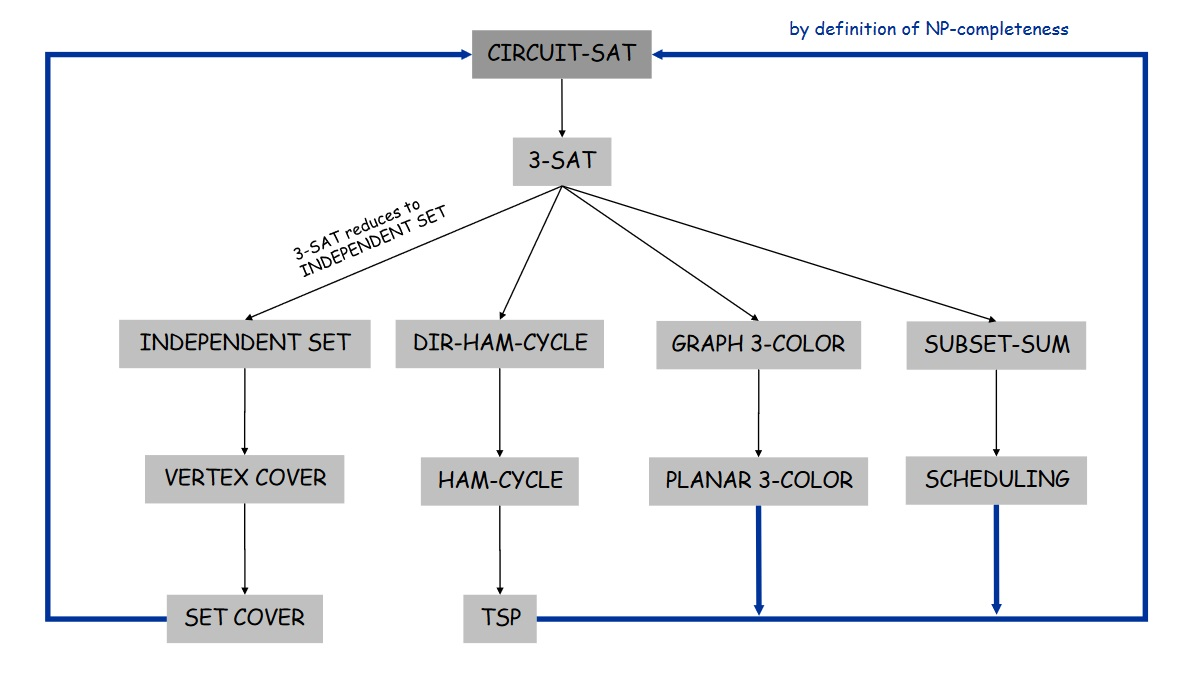
\includegraphics[scale=.75]{NP_Complete}
	\item There are six genres of NP Complete Problems:
		\begin{enumerate}
		\item Packing problems (Set-Packing, Independent Set)
		\item Covering problems (Set-Cover, Vertex-Cover)
		\item Constraint Satisfaction problems (SAT, 3-SAT)
		\item Sequencing problems (Hamiltonian Cycle, Traveling Salesperson)
		\item Partitioning problems (3D-Matching, 3-Color)
		\item Numerical problems (Subset Sum, Knapsack)
		\end{enumerate}
	\item There are some exceptions, like Factoring, Nash Equilibrium in that they don't belong to those genres.
	\item NP Completeness is pretty huge, the biggest thing that enables CS to branch into other disciplines like Mathematics and Economics and so forth.
	\item And there are a \textbf{ton} of different fields by which it is critically important. I encourage you to do some sleuthing of your own to see what can be explored.
	\end{enumerate}
\item So far we've seen Packing, Covering, and Satisfaction NP Problems. Thus, let's look at some more.
\item \textbf{Sequencing Problems}
	\begin{enumerate}
	\item \textbf{Directed Hamiltonian Cycle}
		\begin{enumerate}
 		\item We touched upon it slightly before, but let's revisit it: A \textbf{Hamiltonian Cycle} is a simple cycle (touches a node on its path only once) that contains every node in the graph.
 		\item We know a Hamiltonian Cycle is in NP. 
 		\item But what about a \textbf{Directed} Hamiltonian Cycle? Well, it's actually very easy to show that Ham-Cycle $\leq_{p}$ Dir-Ham-Cycle
 		\item Simply expand the directed graph into an undirected graph by using "mediator" nodes in between cuts of nodes. By doing so, you constrain the pathway and check if each node is touched only once and every node is in the cycle.
 		\item Think of it like this: If there are 3 nodes with edges all pointing at one node, then put in a middle man node between the 3 nodes and the 1 node being pointed to. Then make it undirected between them all. The edges from the 3 nodes should funnel into the middle man node, which should then connect to the other single node, and vice versa. 
 		\item It looks like this: \\
 		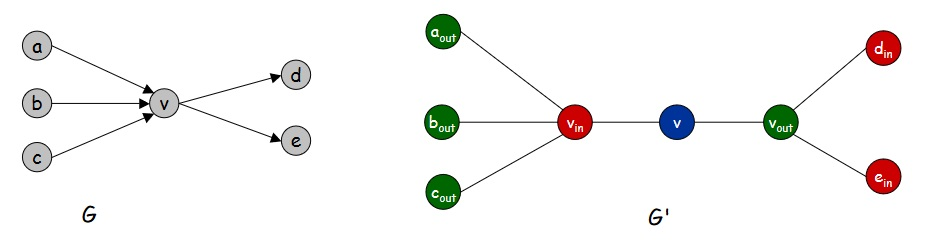
\includegraphics[scale=.85]{Dir_Ham_Graph}
 		\item Finding that a undirected cycle is easy from this, just parse over the nodes as you would with the original Ham-Cycle algorithm.
 		\item Finding/proving that the directed portion works is also simple, because reverting back from undirected edges implies that there must have been an original Ham-Cycle in the first place. 
		\end{enumerate}
	\item \textbf{3-SAT reduces to Directed Hamiltonian Cycle}
		\begin{enumerate}
		\item This is not easy, so bear with me. 
		\item IF a SAT is satisfiable, then construct a Dir-Ham
		\item Construct a graph with $2^n$ Hamiltonian cycles (seriously) such that they map 1-to-1 with truth assignments.
		\item Forma graph with a specific source node $s$, have all combinations of clauses within the middle of the graph between $s$ and a target node at the very end $t$ that will loop back to $s$ for the cycle.
		\item Make the possible combinations of truth clauses in the middle of the graph \textbf{undirected among edges of the same level}.
		\item Each level represents the "state" of each of the literals in a clause. So the first level can be all relative to the literal $x_{1}$. 
		\item Then have nodes that exist outside of this portion that specifically relate to the Clauses themselves. They can act as "placeholders" while the horizontal edges on a level of the graph are parsed. There should be 6 edges in total (3-SAT). This is done specifically not to violate other clauses.
		\item IF by the end of the cycles' circulation there is a satisfied truth assignment that encroaches upon the original graph as directed (with each node touched only once) then huzzah.
		\item It looks like this (from the slides):\\
		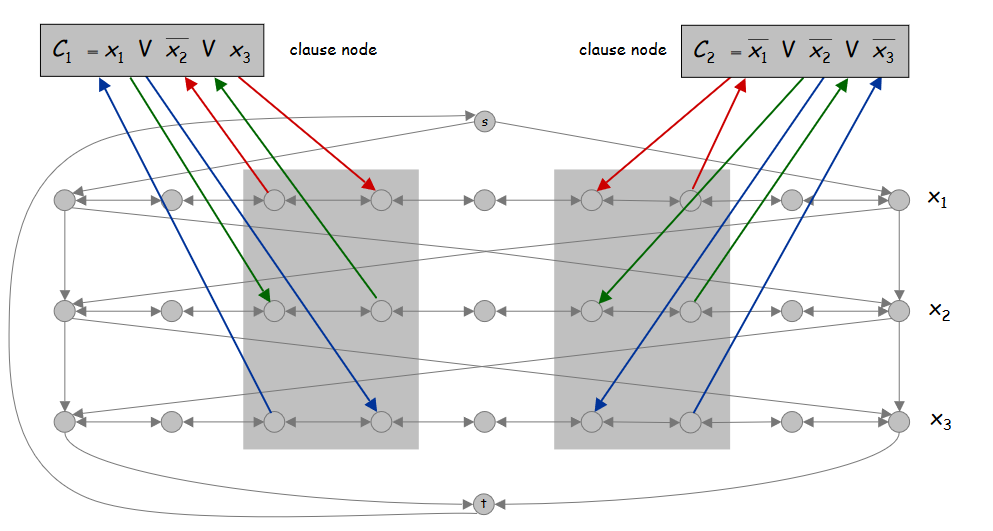
\includegraphics[scale=.85]{3_SAT_Dir_Ham}
		\item I told you working with 3-SAT is terrible. I recommend reading this part over and studying what's actually going on. The first time through doesn't make much sense.
		\item Now time for the fun part -- the Proof:
			\begin{enumerate}
			\item The 3-SAT portion (right direction) is relatively simple:
			\item Traversing a row on the Hamiltonian Graph, if a cycle exists, will have either a value of $1$ going from left to right, or a value of $0$ going from right to left.
			\item This means, each Clause in the graph will have at least 1 row between its 3 literals such that a value can be returned in the correct direction. (If you need a 0, you can get a 0, and if you need a 1, you can get a 1, all based on direction).
			\item The Cycle portion (left direction) is harder:
			\item So, because each row for a clause literal has an outer bound series of "nodes" that it has to go to and from as placeholders, we can assert that if there IS a cycle, the path has to go to these Clause nodes outside of the row, then come back on a different edge (its next edge back from the Clause), and resume at the next node. That means, if we just removed these edges that parse out to the clause, or at the very least normalize their path such that it is basically the same as going from one node to the next node adjacent to it, we can keep the path to only the row.
			\item Then if that is the case, we can traverse a row from left to right and right to left, while maintaining a path that cycles around.
			\item And as the 3-SAT portion of the proof shows, going in a completed direction on a row guarantees a result will be yielded.
			\item So the cycle must exist.  
			\end{enumerate}
		\item Now breathe. If that was very confusing, I don't blame you. I would recommend re-reading the proofs and comparing them with the big graph picture from above, and carefully consider what's happening when the path traverses left and right in a row.
		\end{enumerate}
	\item \textbf{Longest Path}
		\begin{enumerate}
		\item Its name basically says it all. Longest path while touching nodes only once. Like the Shortest Path algorithm, but harder.
		\item We can assert that 3-SAT $\leq_{p}$ Longest Path
		\item Oh god not 3-SAT not again please.
		\item Relax, it's easier this time: First, redo the graph for Directed Hamiltonian Cycle without the edge looping around from the end node to the start node (so as to make sure the cycle doesn't occur)
		\item Then, just show that Ham-Cycle $\leq_{p}$ Longest Path, which is as simple as "A Hamiltonian Cycle has to touch every node, so it has to go over as many edges as possible to do so, and because we remove the cycle edge that loop it back around, its just the longest node from a source to a target"
		\item That wasn't so bad, now was it?
		\end{enumerate}
	\item \textbf{Traveling Salesperson}
		\begin{enumerate}
		\item Given a set of citites, is there a path that travels to each city only once and gets back to the original city by the end that is as shortest as possible?
		\item Essentially just the shortest path from a source to a target that has to touch every node and has to cycle back to the source. No biggie.
		\item Well, we know that Ham-Cycle also has to touch every node and be a cycle...
		\item So we can assert Ham-Cycle $\leq_{p}$ TSP
		\item Proof: With a Ham-Cycle Graph, create "cities" at nodes with a distance function that is given $1$ if the edge between "cities" is in the Ham-Cycle and $2$ if the edge between "cities" is not in the Ham-Cycle.
		\item You are then guaranteed to touch every node and get the "shortest" path distance in the Graph. This will be $\leq$ to the number of nodes in the graph. *Cough* Excuse me,  I meant "cities."
		\end{enumerate}
	\end{enumerate}
\item \textbf{Partitioning Problems} 
	\begin{enumerate}
	\item \textbf{3D-Matching}
		\begin{enumerate}
		\item Given $n$ of instructors, $n$ of courses, $n$ of times and the instructors are clearly defined for what classes they'll teach: Can you set it up so all classes are taught at different times?
		\item So essentially, instructors and courses and times are all disjoint sets of the same size. 
		\item What the final set represents is a series \textbf{triples}, $n$ of them (the same amount as each set). A triple takes the form of [Instructor | Course | Time]
		\item So the question is asking: Can you make a sechdule where each one of these triples is a \textbf{unique} combination when the set of instructos, courses and times are all put in one big bag (Instructors$\cup$Courses$\cup$Times). There can't be any two triples that share, for example, the same instructor at two different times, in the final set.
		\item Hmm....sounds like you are working towards a solution that is a \textbf{set} of \textbf{independent} \textbf{clauses}....
		\item Almost like....you want an \textbf{Independent Set} based around the truth evaluation from a \textbf{3-SAT}
		\item Oh wait. (Yeah ok, I get the snarky sarcasm you can stop now) Sorry, anyways we can show 3-SAT $\leq_{p}$ Independent Set $\leq_{p}$ 3D-Matching
		\item 3-SAT again....this one is a doozy:
			\begin{enumerate}
			\item First, create a gadget for each variable $x_{i}$ (of the 3-SAT form) with "2k core and tip elements"
			\item "What's a 2k core? And tip elements? Are they expensive?" 
			\item "2k core" means that the alternate "clause literals" for a clause are within the gadget edge. A tip element is outstanding truth value for a literal that will be "chosen" by the algorithm
			\item So think of it more this way: If k = 2, then that means each gadget should take the form of a diamond, with 4 triangles conjoined together at the base. 
			\item The "core" of this diamond is dependent on each triangle. Since the triangle base will comprise of 2 elements, the total core will be 4 (2k -> k = 2 -> 2k = 4)
			\item This also means there will be 4 tip elements that represent the chosable elements for truth values. The triangles essentially are created as the triples from the 3D-Matching. 
			\item Also, with the diamond formation, we need to split the color of the triangles in halves: 2 of them red, and 2 of them blue. Why? Because you can only solve the 3D-Matching if the truth values are taken from likewise colored triangles. 
			\item Observe the following picture from the slides, it adheres to the description above: \\ 
			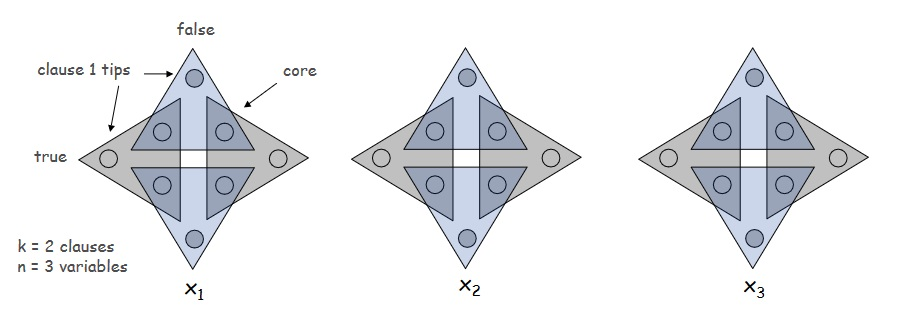
\includegraphics[scale=.85]{3D_Matching}
			\item Notice specifically the orientation of the tips. Each one of them is independent of each other triangle.
			\item However, the elements in the base of the triangles \textbf{are not}. They are double counted by \textbf{different colored triangles}
			\item But remember, 3D-Matching should have no overlap while everything is accounted for. So to account for all 4 elements in the "inner square" of the diamond, you can only select two triangles of the same color.
			\item Now, here's the leap: We need to formulate the actual clauses for the 3-SAT. But how? By linking together tips from different diamonds with 2 other truth values that are completely independent of all the diamonds.
			\item This is a gadget, done specifically to verify a Clause for the 3-SAT.
			\item Here's a picture first, and then I will elaborate: \\
			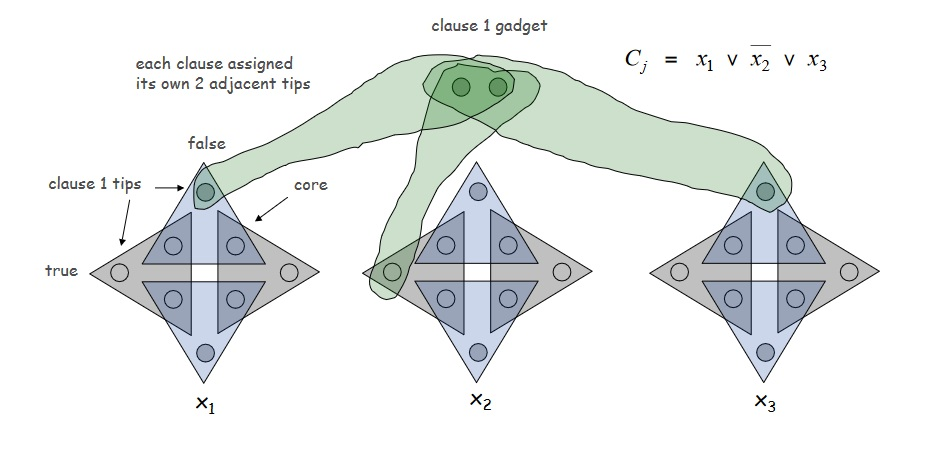
\includegraphics[scale=.85]{3D_Matching2}
			\item Now, notice the two dots in the three-times-overlapped green area? Those elements are generated as an independent clause from 3-SAT. 
			\item $x_{1}$ provides this clause with a TRUE element, which returns a 1 with the clause as is. 
			\item $x_{2}$ provides this clause with a FALSE element, which returns a 2 with the clause. SO, the clause then negates the value from $x_{2}$
			\item $x_{3}$ provides this clause with a TRUE element, which returns 1 with the clause as is.
			\item So we have a satisfiable clause for 3-SAT.
			\item But there's one last thing: There are a bunch of tip elements that are not tracked in the clause. 
			\item Well now what do we do? We provide another gadget, a "Garbage Collector", that cleans up these tips by grouping them also with 2 independent elements. That way 3D-Matching in the non-Independent Set are satisfied. 
			\item Its another extension just like the green one above, but you can make it exclusive, however many times, to each tip element not covered by the green clause. 
			\item And so, finally: \\
			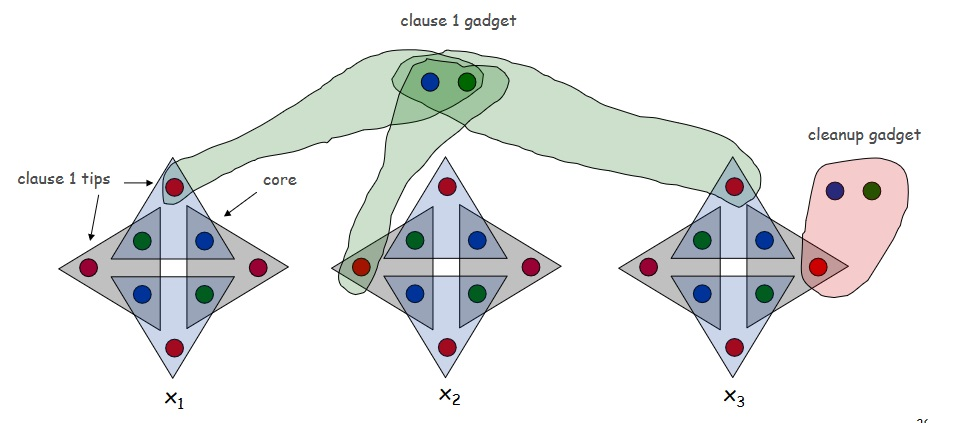
\includegraphics[scale=.75]{3D_MatchingFinal}
			\end{enumerate}
		\item That was a weird one, so if you feel a bit confused don't worry. But this seems like a very important example of how to properly use gadgets for an NP problem, so implore you to read it over and study it carefully. 
		\end{enumerate}
	\item \textbf{Graph Coloring - 3-Colorability} (Remember to bring your crayons)
		\begin{enumerate}
		\item Given an undirected graph, can you color the nodes RGB so that no two adjacent nodes have the same color?
		\item This relates to \textbf{Register Allocation} --> Given a machine with registers, assign programs so that no more than $k$ registers are used and no two programs needed at the same time are assigned to the same register. 
		\item You can build and \textbf{Interference Graph} that basically connects nodes as programs and edges indicate two programs are "active" together.
		\item This is so that you can assert 3-Color $\leq_{p}$ Register Allocation.
		\item Anyhow, back to 3-Color
		\item To show 3-Color we can...show 3-SAT $\leq_{p}$ 3-Color
		\item God I hate 3-SAT. Well, here we go again: 
			\begin{enumerate}
			\item Make a node for every literal.
			\item Make 3 nodes labeled $T$ (True), $F$ (False), and $B$ (Base).
			\item Make negation nodes for every literal node. Connect the literal nodes to their negation nodes.
			\item Connect the TFB in a triangle.
			\item Connect all literal nodes and their negation nodes to the Base node $B$.
			\item Again I'm just going to use the slide pictures for this because they're really good: \\
			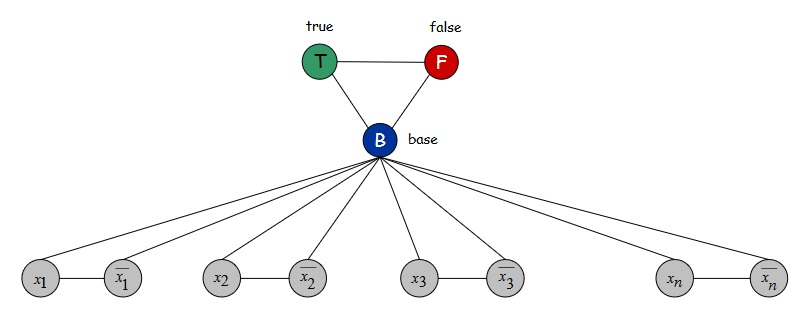
\includegraphics[scale=.85]{3_Color_One}
			\item Via this picture we are absolutely sure all nodes can be alternate colors and the literals can be T/F
			\item Now, to connect to 3-SAT in the most painful way imaginable, add 6 nodes and 13 edges to each Clause. Seriously. \\
			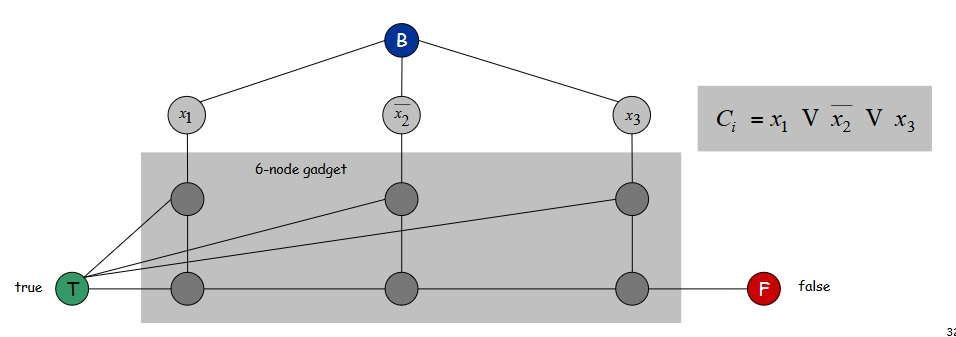
\includegraphics[scale=.85]{3_Color_Two}
			\item Once again, straight from this picture we can see that all nodes can be alternatively colored, literals will be guaranteed T/F, and we will be ensured a truth value in the clause.
			\item Because, if you color all the literals as false, you cannot getting alternation in color nor a truth for the 3-SAT. \\
			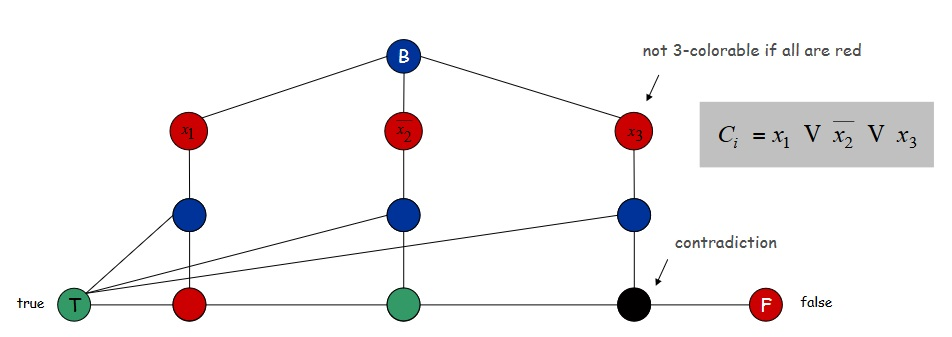
\includegraphics[scale=.85]{3_Color_Three}
			\item And that basically finishes this. Not nearly as complicated as it could have been, but from an explanation standpoint its hard to describe in words.	
			\item I would recommend near memorizing what the pictures are like, or at the very least understand explicitly setting them up. 
			\end{enumerate}
		\end{enumerate}
	\item These NP problems are more about the pictures. Their proofs are far more comprehensive via the pictures than the words, be careful to go over the pictures and study them. 
	\end{enumerate}
\item \textbf{Numerical Problems}
	\begin{enumerate}
	\item \textbf{Subset Sum}
		\begin{enumerate}
		\item Give $n$ set of numbers, and a value $W$, is there a subset of the numbers that adds up to $W$? 
		\item The set of numbers can be all natural numbers by the way. And $W$ can be an countable number likewise. 
		\item We use binary arithmetic for this so the polynomial reduction has to be with binary encoding. 
		\item "What reduction do we use?" you naively ask. I then respond, "Well, with the wonderful incarnation of satan of course. 3-SAT!"
		\item 3-SAT $\leq_{p}$ Subset Sum for the millionth time.
		\item Given a 3-SAT instance, with $n$ variables and $k$ clauses, form $2*n + 2*k$ decimal integers, each of $n+k$ digits in length. 
		\item So if there are $3$ literals, and $3$ clauses, then the integers should be $6$ digits long.
		\item This process can "create" digits by operating in binary and setting bits according to the literals and the clauses. 
		\item That is, if the table is [x1 | x2 | x3 | C1 | C2 | C3], then a binary value can be assigned to each variable in according with an integer (byte size per each of the 6 variables) 
		\item Here's a table from the powerpoint to simplify this: \\
		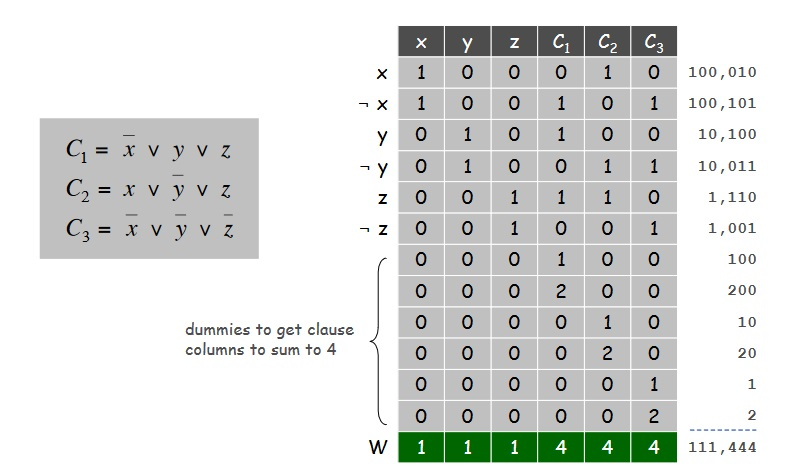
\includegraphics[scale=.85]{Subset_Sum}
		\item That's essentially its own proof, the logic of it is intuitive although it may not seem so at first. After a second or third glance at it, it becomes pretty obvious what's ocurring.
		\end{enumerate}
	\item \textbf{Scheduling (With Release Times)}
		\begin{enumerate}
		\item Given a set of jobs ($n$ jobs), each with a processing time, a release time, and a deadline, it is possible to schedule \textbf{all} jobs on one machine such that each job runs from release to deadline during its process time without interuption?
		\item So, to reduce it we use...not 3-SAT? Oh thank goodness.
		\item Subset Sum $\leq_{p}$ Schedule w/ Release Times (Although, because 3-SAT $\leq_{p}$ Subset Sum, by transitive property 3-SAT $\leq_{p}$ Schedule. You can go ahead do that yourself if you'd like :D )
		\item Given a Subset Sum with a set of integers of $w_{1}...w_{n}$ and a target integer $W$, create $n$ jobs with a processing time $t_{i} = w_{i}$, release times of $0$, and no preemptive deadlines.
		\item The deadlines just become the processing time + the last point where the prior job finished. 
		\item The first job, $job_{0}$, should have processing time of $1$, a release time of $W$, and a deadline of (processing + release = $W+1$).
		\item Now, the places to put jobs are: Anywhere from 0 to $W$ and $W+1$ to the end of the schedule. 
		\item And then this continues in likewise D\&Q type fashion.
		\end{enumerate}
	\item So numerical NP problems seem to be about how to represent the integers or ordering of elements/jobs. And specifically how they relate to their reduction.
	\end{enumerate}
\item Just about done with the chapter, but a last few small things:
\item We \textbf{will continue to talk about NP problems} in the following chapters, but in different contexts and more about the problem rather than the reduction/how it's NP.
\item The biggest takeaway of NP is that reductions are all about showing that the Problem on the Left is just a solvable case of the Problem on the Right. The proofs and examples are specifically to show how reductions work. But understanding the overall relevance of a reduction is the most important thing, not just the proofs. 
\item And I have one final spew about NP, pertaining to NP Completeness
\item \textbf{NP Hard vs NP Complete}
	\begin{enumerate}
	\item \textbf{NP Complete is a subset of NP Hard}
	\item Here's a table: \\
		\begin{tabular}[c]{c|c}
		NP-Hard & NP-Complete \\
		\hline 
		Is in NP & Is in NP \\ 
		NP Based $A$ exists where $A \leq_{p} B$ & All NP Complete $A$ exist where $A \leq_{p} B$ \\ 
		Do not always reduce to one another & All NP Complete reduce to other NP Complete \\ 
		\end{tabular}
	\item Here's a picture of how the space for NP works. \\
	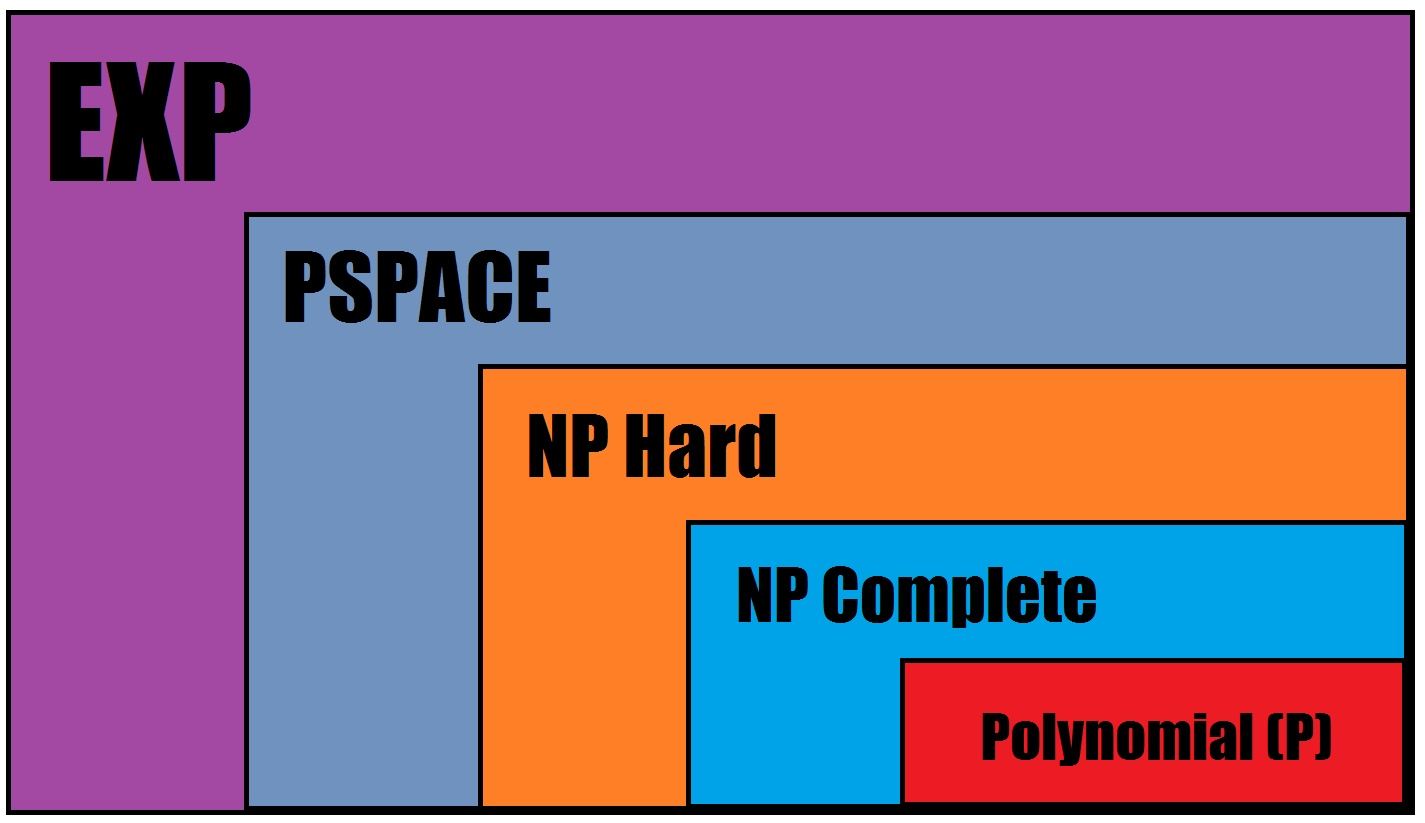
\includegraphics[scale=.4]{NP_SUBSET_TWO}
	\item Please note: There are a gazillion more "problem spaces" that are all over the place and I do not have the time nor am insane enough to make an image to go that in-depth. We aren't really even covering PSPACE or EXP.
	\end{enumerate}  
\item And one last tiny thing: NP Complete problems do have a "hierarchy" of sorts. Specificaly, 3-SAT reduces to \textbf{every other freaking NP Complete} problem, so when in doubt, you can always go back to 3-SAT for an NP Complete reduction. 
\item And that ends the chapter for NP and Intractibilty. If you survived, then congratulations! Here's your warm milk and cookie, enjoy your comfortable sleep tonight. If you didn't, well fear not, others will dwell with you in the darkness of Niflheim.
\end{enumerate}

\vspace{1em}
\subsection*{Local Search}
\begin{enumerate}
\item So you have an NP Hard problem, huh? And you won't to solve it? Well, theory isn't really on your side, now is it? Going to be pretty hard to solve in properly, in a timely fashion, at any given time.
\item But you've got to solve it, huh? Well, then, you can do so, but \textbf{at a cost}
\item This chapter is about solving really hard problems in the best feasible way (as of now) possible. And these are \textbf{Heuristics}: techniques for formulating algorithms for difficult problems in the best way possible. Specifically, these will be covering algorithms that forfeit optimality in favor of completion. 
\item But you must forefeit one of the following:
	\begin{enumerate}
	\item Solving for the optimal solution.
	\item Solving in polynomial time.
	\item Solving any arbitrary instance of a problem (i.e. making your algorithm as general as possible)
	\end{enumerate}
\item \textbf{Landscape of an Optimization Problem}
	\begin{enumerate}
	\item \textbf{Gradient Descent: Vertex Cover}
		\begin{enumerate}
		\item You want to solve an NP problem, Vertex Cover
		\item An "algorithm" for doing so would \textbf{Gradient Descent}
		\item Before this, remember what vertex cover is -- a subset of nodes in a graph that touches every edge and is minimized.
		\item And a \textbf{neighbor relation} is another set of nodes that is 1 greater or 1 less than the Vertex Cover set (delete or add a node)
		\item So with those defined, a \textbf{Gradient Descent} is very simple: Initiate the "vertex cover" set to be all nodes in the graph.
		\item Then check if there is a neighboring set that is both 1) smaller and 2) is a vertex cover
		\item If so, replace the vertex cover set with this neighbor set.
		\item Think of it like this: There are 5 nodes in the full set. There's a neighbor that is 4 nodes and is a vertex cover. The new full set is the 4 nodes. And this process can continue until, at worst, every node has been deleted ($n$ steps, which is the total number of nodes)
		\item This algorithm somwhat forfeits optimality, because the optimal solution might be an odd orientation where the strict neighbors doesn't account for. 
		\item Say if you have a line of nodes, then every other node would be the optimal solution because every other node would touch both edges incoming and outgoing. 
		\item Thus, this is a \textbf{Local Search}: an algorithm that explores possible outcomes by finding the "next best/nearby" solution to the current one in sequential fashion.
		\item In the context of gradient descent: If there is a current working solution, check if there is neighbor solution with a lower cost, and replace the current solution with the smallest possible of lower costs. Else terminate. 
		\end{enumerate}
	\end{enumerate}
\item \textbf{Metropolis Algorithm}
	\begin{enumerate}
	\item Physical energy states (low and high), with a biased operation for downhill (read: easier) steps, but can do uphill.
	\item Algorithm is all about maintaining a given state, by feeding it "easy" operations most of the time and occasionally "hard" operations to offset it. 
	\item The right amount of time and states will be found by the end of execution. 
	\item This concept of balancing Energy states with lows and highs lends to the construct of \textbf{Simulated Annealing}
	\item \textbf{Simulated Annealing}
		\begin{enumerate}
		\item $T$ Large => probability of a "hard" move is large.
		\item $T$ Small => probability of a "hard" move is small.
		\item Idea: Find a good balance of $T$ Large and $T$ Small to maintain a given input state.
		\item Cooling Schedule: Every iteration of some element or space, $T$ gets switched. 
		\end{enumerate}
	\item The breakdown is like this: Take a solid and melt it really quickly, then take a molten solid and freeze it really quickly.
	\item And then Annealing: Gradually cool from high temperatures so that the structure evens out / reaches equilibrium.
	\end{enumerate}
\item \textbf{Hopfield Neural Networks}
	\begin{enumerate}
	\item Simulating an associative memory: neighbors in a network try and correlate/assume the states of one another.
	\item The graph configuration is simple: given a graph with integer weights, add nodes with weights that are either positive or negative $1$. 
	\item If the edge weight between nodes is negative, then the nodes should be the same "state". If the edge weight between nodes is positive, then the states should be different.
	\item An edge is \textbf{good} if the edge weight is negative and the nodes share states.
	\item An edge is \textbf{bad} if the edge weight is negative and the nodes differ in states.
	\item This also works with positive edge weights (good if differ in states, bad if same state).
	\item A node is \textbf{satisifed} if the sum of good edges (from the node) is greater than the sum of bad edges (from the node).
	\item \textbf{State Flipping Algorithm}: Repeatedly flip the state of an unsatisfied node. (While the graph is unsatisfied, go through nodes and flip their states)
	\item This algorithm will operate in the space of the total amount of edges in the graph. 
	\item Proof:
		\begin{enumerate}
		\item Let $S$ be the number of satisfied nodes. 
		\item Let $W$ be the total amount of edge.
		\item Obviously $0 \leq S \leq W$ because worst case all nodes are unsatisfied and there will still be less than or equal to the total edges.
		\item After each flip: All good and bad edges that \textbf{touch the node} flip (good becomes bad and vice versa). All other edges and nodes in the graph maintain their weight and states. 
		\item We can show that: ($S$ - Sum of good edges + Sum of bad edges) is $\geq$ $S+1$. The inequality represents the existence of unsatisfied nodes.
		\end{enumerate}
	\item Notice the distinction between what the original probem is asking:
		\begin{enumerate}
		\item Search Problem: Given a weighted graph, find a configuration for the Hopfield Neural Network.
		\item Decision Problem: Given a weighted graph, is there a stable configuration? 
		\end{enumerate}
	\item The decision portion is polynomial solvable, but the search problem is not known.
	\end{enumerate}
\item \textbf{Maximum Cut}
	\begin{enumerate}
	\item Given a weighted graph with positive integer edges, find a cut of nodes where the flow/sum of weights is maximized.
	\item There are some practical applications for this (Person-Activity scheduling, Circuit layout, statistical physics)
	\item Algorithm:
		\begin{enumerate}
		\item Greedily pick a random partition of nodes into segment $A$ and segment $B$.
		\item Continually choose nodes from each segment and swap the node into the other segment to maximize/improve the parition weight.
		\item Once the best possible weight is achieved from the cut, return the segments.
		\end{enumerate}
	\item The proof is awkward, so here's a verbal explanation:
		\begin{enumerate}
		\item The locally optimal solution (that we found) is greater than or equal to half the sum of all edges weights.
		\item We know that with local solutions we forfeit some optimality, so the sum of segment $A$ is $\leq$ than segment $B$.
		\item This means that the sum of segment $A$ is $\leq$ the local optimal solution. ($w(A, B)$)
		\item And we also know that the sum of segment $B$ is $\leq$ the local optimal solution. ($w(A, B)$)
		\item So then [the sum of segment $A$] + [the sum of segment $B$] + [the local optimal solution ($A + B$)] is $leq$ the local optimal solution times two. $2*w(A, B)$
		\item But we know that $2*w(A, B)$ is the sum of all edges anyhow (the parition is a cut of half the edges essentially), so we have the best local optimal solution.
		\end{enumerate}
	\item Local optimal solution versus the universal optimal solution (which is too hard to find) is an important distinction here.
	\item The time complexity for this local search version is still not polynomial completion, however. 
	\item Using \textbf{Big Improvement Flips} will provide a better time.
	\item The algorithm is the same as the local search version, but it only swaps nodes between segments if it improves the solution $w(A, B)$ by $2\varepsilon /n$ where $n$ is the number of nodes. ($\varepsilon$ is an arbitrary increase by some value)
	\item The proof is also the same, just with $2\varepsilon /n$ attached to each sum of segments.
	\item This algorithm terminates in $\varepsilon * n * log($Sum of edge weights$)$
	\item There are 50\% and 87\% approximation algorithms for Max-Cut, but if P != NP then there is no algorithm better than 95\% approximation.
	\end{enumerate}
\item More on \textbf{Neighbor Relations}: We discussed \textbf{1-Flip}, but \textbf{k-flip} means essentially the same thing except that the nodes are $k$ flips different, not just 1-flip. $\Theta{n^k}$
\item Implementing this in \textbf{KL-Neighborhood} format means marking "flipped" nodes. 
\item Marking of nodes is extremely useful in practice and in theory, helping to avoid excess node flips and increase execution operations.
\item Now, the final problem of the chapter is \textbf{Nash Equilibria}
	\begin{enumerate}
	\item \textbf{Multicast Routing} --> Directed graph with a source node, a series of other nodes that are path ends, and edges with integers that are $\geq 0$. 
	\item An \textbf{agent} $j$ will find a path from the source node to a path end node $t_{j}$, paying the edge costs as it goes. 
	\item Agents will always switch to the best path available for them depending on other agents.
	\item Agents pay the integer value of a path divided by how many other agents are using it.
	\item \textbf{Nash Equilibrium} --> Solution where agents have their best paths satisfied.
	\item Local Search approaches: Agents continually jump edges depending on other edges, looking for the best path possible for them.
	\item \textbf{Socially optimal} solutions are rendition of Nash Equilibria if the cost of all agents in minimized.
	\item There can be many form of the Nash Equilibria, and they aren't always socially optimal.
	\item Stabilizing an algorithm/problem between Nash Equilibria and Social Optimality comes at a price of $\Theta{log(k)}$
	\item The algorithm for Nash Equilibrium has basically been said: Pick a path for an agent, and while an Equilibria has not been reached, pick an agent for the path and switch it to a path that improves the solution.
	\item The proof is actually extremely intuitive (despite dense mathematical notation on the slides): Basically, by switching an agent to a new path, there's a new total cost less than the cost before it because a cheaper pather was switched to. This occurs for all agents until a Nash Equilibria is achieved.
	\item Of course, this is all based around countably infinite sized edges in cost. (back to the stabilizing issue)
	\item So the worst Nash Equilibria you can devise that is worse than the social opmtimum is at most the size of the countable agent space for the problem. 
	\item Summary for Nash:	
		\begin{enumerate}
		\item Existence: Nash Equilirbia will always exist for a routing problem about agents that prioritize sharing path lengths (finding the best possible for each)
		\item The best Nash is never worse than the social optimum by greater than the agent problem space size
		\item The hard part in all of this is finding a Nash Equilirbia in polynomial time.
		\end{enumerate}
	\end{enumerate}
\item And that is it for this chapter. The algorithms all base around the concept of local search -- finding the next best thing to what you already have -- and deriving agorithms for hard problems in doing so.
\end{enumerate}

\vspace{1em}
\subsection*{Approximation Algorithms}
\begin{enumerate}
\item So much like the Local Search chapter, this chapter will also work on solving NP problems in reasonable time.
\item But unlike the Local Search Chapter, these \textbf{Approximation Algorithms} will:
	\begin{enumerate}
	\item Run in polynomial time
	\item Solve any instance of the problem
	\item Find a solution within a ration $\delta$ of true optimality (the solution ratio is $\leq 1$). This part is weird because we may not even know what the true optimal solution is, so proving it is tough.
	\end{enumerate}
\item So these are really good and pretty important.
\item \textbf{Load Balancing}
	\begin{enumerate}
	\item A type of job scheduling problem with a requirement that all jobs get scheduled.
	\item All about maximizing machine scheduling of the jobs.
	\item It has the following variables:
		\begin{enumerate}
		\item $n$ jobs
		\item $m$ machines
		\item $t$ processing time, which is really just the space it takes up in the available space in the schedule
		\item There is a \textbf{makespan}: a maximum load -- amount of jobs you can assign to -- any machine
		\end{enumerate}
	\item Firstly, before covering it specifically, we should ask: is this problem in NP?
	\item Recall back to the original job scheduling problem, in which you only scheduled the best possible jobs. It was solved Greedily by taking the shortest job available, and then inputting the next legal available job after it finished.
	\item The approximation goal is essentially to minimize the makespan by assigning jobs accordingly.
	\item The Approximation Algorithm: 
		\begin{enumerate}
		\item Fix some order of the given $n$ jobs
		\item Take each job sequentially.
		\item Place each job into a machine with the least processing time (most space) available.
		\item The algorithm's implementation runs in $O(n*log(n))$ time.
		\end{enumerate}
	\item Before analyzing the algorithm, let's show a reduction:
	\item \textbf{Subset Sum $\leq_{p}$ Load Balancing}
		\begin{enumerate}
		\item IF there is a partition of the Subset Sum, then....
		\item There is a solution of the Load Balancing if job $L_{1}$ = job $L_{2}$
		\item The corresponding machines liken to the two sets of integers [$w_{j} = w_{i}$ <==> $L_{j} = L_{i}$] 
		\end{enumerate}
	\item Decision version of this problem: Given $K$, is there a schedule such that the makespan $\leq K$
	\item $K$ is identified as: $\frac{\sum_{i=0}(w_{i})}{2}$
	\item Side note: You must show the certificate that the problem is NP Hard/Complete. Remember a certificate is just a way of showing it can or can't work.
	\item Analysis of the Algorithm: 
		\begin{enumerate}
		\item Consider $L'$ to be the optimal solution. 
		\item We should find lower bounds for it.
		\item $L' \geq max_{j}*t_{j}$ -- This works because some machine has to take on the biggest job
		\item $L' \geq \frac{1}{m}*\sum_{j}t_{j}$ -- This works via pigeonhole principle: at least one machine will be stuck with the job if there is a greater amount of jobs than machines.
		\item This means the greedy algorithm is 2-Approximation 
		\end{enumerate}
	\item Proof of 2-Approximation:
		\begin{enumerate}
		\item Consider load $L_{i}$ of a bottleneck machine $i$
		\item When job $j$ is assigned to machine $i$, $i$ had to have the smallest load. Its load before the assignment was $L_{i} - t_{j}$ which is $\leq L_{k}$ for all values where $1 \leq k \leq m$
		\item So we have to show $L_{i} \leq 2*L'$ (this is a theorem)
		\item With the sum of the inequalities on machines, we then get $m * L_{i} - t_{j} \leq \sum_{k}L_{k}$, and we can move the $m$ over to $\frac{1}{m}\sum{k}L_{k}$
		\item This sum $\sum_{k}L_{k}$ is less than $L'$. 
		\item So, $L_{i} - t_{j} \leq \frac{1}{m}\sum{k}L_{k} \leq L'$
		\item You can then logically connect that $\frac{1}{m}\sum{k}L_{k} + L' \leq L' + L'$
		\item And $L_{i} - t_{j}$ was based around $\sum{k}L_{k}$, so we can just use $L_{i}$
		\item Then finally: $L_{i} \leq 2*L'$
		\end{enumerate}
	\item Point is, we used the instance of the last job to define a proper upperbound ($2*L'$) that verifies the original issue in the proof (the theorem really)
	\item Be wary of tightening the analysis of an approximation
	\item A variant of this problem is instead to take the longest processing time by order, called the \textbf{LPT Rule}
	\item It also runs in the same time $O(n*log(n))$ and it is better because it is a $\frac{3}{2}$ Approximation
	\item Quick Proof of this new Approximation:
		\begin{enumerate}
		\item Theorem of: $L_{i} \leq \frac{3}{2}*L'$
		\item Order machines in decreasing process time.
		\item After $m$ jobs scheduled, the last one has the shortest processing time (most space available).
		\item $m+1$ is thereforegoing to be the smallest job across all existing jobs on the machines
		\item The same math proof from above would work equally, with the simple diffence being the $\frac{3}{2}$ versus the 2
		\end{enumerate}
	\item This analysis isn't fully tight, but there is a basis there for tight analysis and algorithm completion.
	\end{enumerate}
\item \textbf{Center Selection}
	\begin{enumerate}
	\item Finding the best possible center "site" such that the distance between all other sites in minimized.
	\item Best to think in terms of a Circle's area. 
	\item Using the concept of dist(x, y) -- which represent the distance between x and y -- we can define the following:
		\begin{enumerate}
		\item dist(x, y) => 0 (identity)
		\item dist(x, y) => dist(y, x) (symmetry)
		\item dist(x, y) $\leq$ dist(x, z) + dist(z, y) (triangle inequality)
		\end{enumerate}
	\item dist($s_{i}$, C) = min(c$\in$C) dist($s_{i}$, c) = distance from $s_{i}$ to closest center.
	\item (C) = $max_{i}dist(s_{i}, C)$ = smallest covering radius.
	\item So the end game is to find the smallest possible r(C), such that the cardinality of |C| => k
	\item Using random Euclidean points as centers can be infinite, so that's no good.
	\item Using a greedy approach by centering one as "best" and then adding accordingly is bad for arbitrary growth.
	\item Better Greedy Approach:
		\begin{enumerate}
		\item Set a center in the best possible space to begin
		\item Then repeatedly set centers farthest away from any existing center as possible.
		\item By the construction of the Algorithm, by the end it will be pairwise r(C)
		\end{enumerate}
	\item The proof is a contradiction that asserts that $r(C) \leq 2r(C*)$
		\begin{enumerate}
		\item By asserting that a radius $\frac{1}{2}r(C)$ around, then the pairing for centers in the circle 
		\item Must be thus that the new pairing is less than what was there.
		\end{enumerate}
	\item Theorems are: $r(C) \leq 2r(C*)$ and Greedy Algorithm is 2-Approximation
	\item There is no hope of $\frac{3}{2}$ or $\frac{4}{3}$ approximation unless P = NP
	\end{enumerate}
\item Pricing Method: Vertex Cover
	\begin{enumerate}
	\item Find a Vertex cover with minimum weight.
	\item Essentially, find each price such that it is $\geq$ 0 but also per edge such that the total price $\leq$ than the total weight.
	\item Just find a Vertex Cover of the prices. 
	\item Another 2-Approximation, with verification of termination as there become fewer available nodes after a cover node is confirmed.
	\end{enumerate}
\item LP Rounding: Vertex Cover
	\begin{enumerate}
	\item With an undirected, weighted graph, find the minimum cover with each node has at least one edge incident in the cover.
	\item Can use a binary representation for "in/out" of the Vertex cover. 
	\item So, by searching the 1-1 correspondence, you can maximize the weight with vertex that exist in the cover.
	\item (Integer Programming) $\sum(w_{i}*x_{i})$
		\begin{enumerate}
		\item $x_{i}$ => ${0,1}$ ($i \int V$)
		\item $x_{i}+x_{j} \geq$ (1) ($i, j \in V$)
		\end{enumerate}
	\item If $x*$ is optimal in the \textbf{Integer Programming Formulation}, then S is a min weight vertex cover.
	\item Happens that finding a representation given integer $a_{i,j}$ and $b_{i}$ is a NP-Hard reducible process to Vertex Cover.
	\item \textbf{Linear Programming} allows for both solvable and polynomial assertions with input of integers $c_{j}$, $b_{i}$, and $a_{i,j}$
	\item The tradeoff is that the accurracy of the Linear Programming is less than that of the Integer Programming. 
	\item LP is also not equivalent to a Vertex Cover, unless we solve for rounded fractions.
	\item All tolled, this is a 2-Approximation algorithm.
	\item If P != NP, then p-approximation can be no less than 1.3607
	\end{enumerate}
\item \textbf{Load Balancing Reloaded}
	\begin{enumerate}
	\item Another walk through job scheduling problem
	\item Set of $m$ machines, and $j$ jobs, with each job having a processing time $t$
	\item The difference with the other Load Balancing is by what machines are \textbf{authorized} to take on a job.
	\item All the proofs from a general standpoint are the same.
	\item You can do the more specified authorization with IP Formulation and Linear Programming. \\
	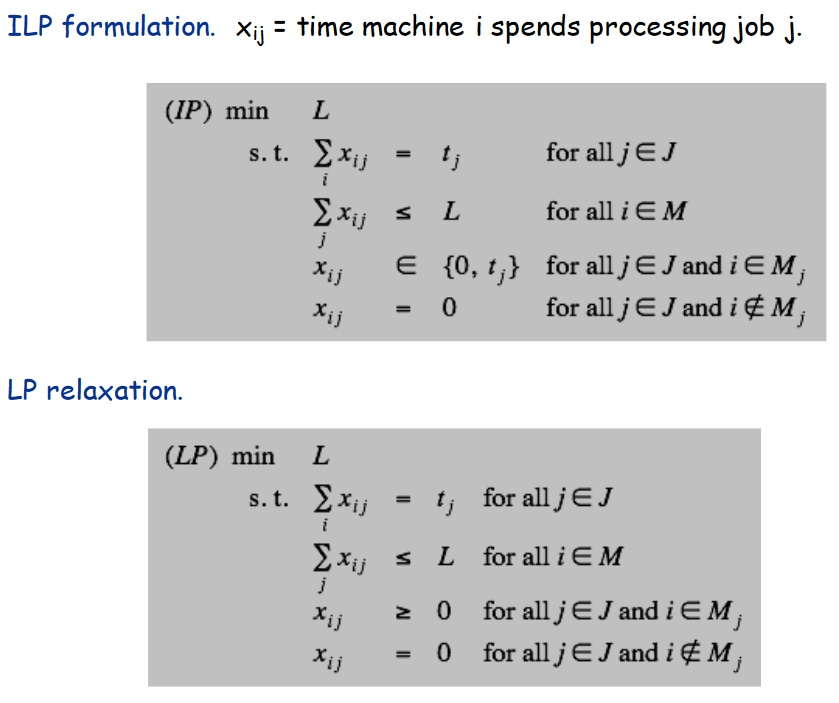
\includegraphics[scale=.85]{Load_Balancing_Reloaded}
	\item The \textbf{Lower Bound} formulation will be an optimal makespan via an acyclic graph construction.
	\item A \textbf{rounded} solution is also based off the graph formulation, verifying authorizedmachines because only positive values can be authorized. 
	\item Also, another item is that if a job is a leaf in this acyclic graph and the machine is a parent, the job is a culmination of authroized processes to this job. 
	\item The solution (rounded) is 2-Approximation because the sum of times of a leaf node (that is a job) is the sum of authorized job processes to that point. And that is $\leq$ the LP Relaxation that it is a minimized makespan.
	\item Conclusion:
		\begin{enumerate}
		\item Running time is the solution for Linear Programming in $m*n+1$.
		\item Can solve this LP with flow techniques on a graph.
		\end{enumerate}
	\end{enumerate}
\item \textbf{Knapsack Problem}
	\begin{enumerate}
	\item We talked about this before, you have a bag with weights and you have things you want to put in it, maximize the value you can put into it while staying in capacity.
	\item We tackled this with Dynamic Programming initially.
	\item We can analyze this via rounding and scaling in this chapter.
	\item First, \textbf{Subset Sum $\leq_{p}$ Knapsack}. Pretty straightforward: With a "target" value and the given weight capacity, find a set arrangement of nonnegative integers. The values are integers from a Subset Sum. 
	\item So the dynamic programming implementation (way up above) has a running time $O(n*W)$ where $W$ is a Weight capacity. But as remarked before, $W$ repetitively can be huge, and so it won't run in polynomial time.
	\item So changing the dynamic programming to a min weight subset that yield exacts a value from the knapsack, rather than bound the weight capacity, might increase time, right?
	\item Nope. The running time becomes $O(n^2 *$ max(v)$)$
	\item Approximation Algorithm:
		\begin{enumerate}
		\item Round all values up to lie in smaller ranges
		\item Run the dynamic programming on the rounded values
		\item Return the optimal values from the rounded instance
		\end{enumerate}
	\item The rounding is virtually incremental, or at least within a reasonable bounds, so that the true values are not completely off. 
	\item Although optimality would have been suffered, the running time becomes $O(n^3 / \varepsilon)$
	\item The proof is essentially a turning of the sum into \\ $\sum_{i \in Solution}\bar{v_{i}} \\ \leq \sum_{i \in Solution}(v_{i} + \Theta) \\ \leq \sum_{i \in Solution}(v_{i} + n*\Theta) \\ \leq (1+\varepsilon) * \sum_{i \in Solution}v_{i}$
	\item Which is basically all just saying the difference in value growth within the Capacity solution is incrementally altered by at most $\varepsilon$
	\end{enumerate}
\item And that ends this chapter. Tad bit quicker than the other chapters, and essentially wraps up the class. The main portion from this chapter is just about practical creation of an aglorithm for some really difficult NP problems. Not far from the chapter prior.
\end{enumerate}

\vspace{2em}
\noindent \textbf{Final Remarks}\\
\indent And that ends the notes! I hope they were helpful, they were a back and forth between the slide notes and my own personal notes from lectures. They seem to capture the general idea of everything we covered, although some parts are less obvious then others. I suggest it useful to review the slide notes in juxtaposition with the notes in this PDF. But my hope is that this is comprehensive enough for your own benefit. And I apologize if there are grammatical errors, no autocorrect makes catching them tough.

\end{document}
